%
% neldermead.tex --
%   Some notes about Nelder-Mead algorithms.
%
% Copyright 2008-2009 Michael Baudin
%
\documentclass[12pt]{report}

%% Good fonts for PDF
\usepackage[cyr]{aeguill}

%% Package for page headers
\usepackage{fancyhdr}

%% Package to include graphics
%% Comment for DVI
\usepackage[pdftex]{graphicx}

%% Index
\usepackage{makeidx}
\makeindex

%% Figures formats: jpeg or pdf
%% Comment for DVI
\DeclareGraphicsExtensions{.jpg,.pdf}

%% Package to create Hyperdocuments
%% Comment for DVI
\usepackage[pdftex,colorlinks=true,linkcolor=blue,citecolor=blue,urlcolor=blue]{hyperref}

%% Package to control printed area size
\usepackage{anysize}
%% ...by defining margins {left}{right}{top}{bottom}
\marginsize{22mm}{14mm}{12mm}{25mm}

%% Package used to include a bibliography
\usepackage{natbib}

%% R for real numbers
\usepackage{amssymb}

%% User defined commands

%% Figure reference
\newcommand{\figref}[1]{figure~\ref{#1}}

%% Equation reference
\newcommand{\Ref}[1]{(\ref{#1})}

%% Emphasize a word or a group of words
\newcommand{\empha}[1]{\textit{\textbf{#1}}}

%% Derivation operators
\newcommand{\D}{\partial}
\newcommand{\Dt}{\partial_t}
\newcommand{\Dx}{\partial_x}
\newcommand{\Dy}{\partial_y}

\newcommand{\bv}{\mathbf{v}}
\newcommand{\bx}{\mathbf{x}}
\newcommand{\bl}{\mathbf{l}}
\newcommand{\br}{\mathbf{r}}
\newcommand{\bg}{\mathbf{g}}

\usepackage{url}

% Scilab macros
\newcommand{\scifunction}[1]{\textit{#1}}

% To highlight source code
\usepackage{listings}

\lstdefinelanguage{scilabscript}%
  {morekeywords={abcd,abinv,abort,abs,acoshm,acosh,acosm,acos,addcolor,%
      addf,addinter,addmenu,add_edge,add_node,adj2sp,adj_lists,aff2ab,%
      amell,analpf,analyze,ans,apropos,arc_graph,arc_number,argn,arhnk,%
      arl2,arma2p,armac,armax1,armax,arma,arsimul,artest,articul,ascii,%
      asinhm,asinh,asinm,asin,atanhm,atanh,atanm,atan,augment,auread,%
      auwrite,balanc,balreal,bandwr,basename,bdiag,besseli,besselj,%
      besselk,bessely,best_match,bezout,bifish,bilin,binomial,black,%
      bloc2exp,bloc2ss,bode,bool2s,boolean,boucle,break,bstap,buttmag,%
      bvode,cainv,calerf,calfrq,call,canon,casc,case,ccontrg,cdfbet,%
      cdfbin,cdfchi,cdfchn,cdffnc,cdff,cdfgam,cdfnbn,cdfnor,cdfpoi,%
      cdft,ceil,center,cepstrum,chaintest,chain_struct,champ1,champ,%
      chart,chdir,cheb1mag,cheb2mag,check_graph,check_io,chepol,chfact,%
      chol,chsolve,circuit,classmarkov,clean,clearfun,clearglobal,%
      clear,close,cls2dls,cmb_lin,cmndred,cmoment,code2str,coeff,coffg,%
      coff,colcompr,colcomp,colinout,colormap,colregul,companion,comp,%
      cond,conj,connex,contour2di,contour2d,contourf,contour,%
      contract_edge,contrss,contr,cont_frm,cont_mat,convex_hull,convol,%
      convstr,con_nodes,copfac,copy,correl,corr,coshm,cosh,cosm,cos,%
      cotg,cothm,coth,covar,csim,cspect,ctr_gram,cumprod,cumsum,%
      curblock,cycle_basis,czt,c_link,dasrt,dassl,datafit,date,dbphi,%
      dcf,ddp,debug,dec2hex,deff,definedfields,degree,delbpt,%
      delete_arcs,delete_nodes,delete,delip,delmenu,demos,denom,%
      derivative,derivat,des2ss,des2tf,determ,detr,det,dft,dhinf,%
      dhnorm,diag,diary,diff,diophant,dirname,dispbpt,dispfiles,disp,%
      dlgamma,double,dragrect,drawaxis,drawlater,drawnow,draw,driver,%
      dscr,dsearch,dsimul,dtsi,dt_ility,duplicate,edge_number,%
      edit_curv,edit_graph_menus,edit_graph,edit,eigenmarkov,ell1mag,%
      elseif,else,emptystr,endfunction,end,eqfir,eqiir,equil1,equil,%
      ereduc,erfcx,erfc,erf,errbar,errcatch,errclear,error,eval3dp,%
      eval3d,eval,evans,evstr,excel2sci,execstr,exec,exists,exit,expm,%
      exp,external,eye,fac3d,factors,faurre,fchamp,fcontour2d,fcontour,%
      fec,feedback,feval,ffilt,fftshift,fft,fgrayplot,figure,fileinfo,%
      file,filter,findm,findobj,findx0BD,find_freq,find_path,find,%
      findABCD,findAC,findBD,findBDK,findR,fit_dat,fix,floor,flts,foo,%
      formatman,format,fort,for,fourplan,fplot2d,fplot3d1,fplot3d,%
      fprintf,fprintfMat,frep2tf,freq,freson,frexp,frfit,frmag,fscanf,%
      fscanfMat,fsfirlin,fsolve,fspecg,fstabst,fstair,ftest,ftuneq,%
      fullrfk,fullrf,full,fun2string,funcprot,functions,function,%
      funptr,fusee,gainplot,gamitg,gammaln,gamma,gcare,gcd,gcf,%
      genfac3d,genlib,genmarkov,gen_net,geom3d,geomean,getblocklabel,%
      getcolor,getcurblock,getcwd,getdate,getd,getenv,getfield,getfont,%
      getf,getio,getlinestyle,getmark,getpid,getscicosvars,getsymbol,%
      getvalue,getversion,get_function_path,get,gfare,gfrancis,girth,%
      givens,glever,glist,global,glue,gpeche,graduate,grand,%
      graphics_entities,graph_2_mat,graph_center,graph_complement,%
      graph_diameter,graph_power,graph_simp,graph_sum,graph_union,%
      graph-list,graycolormap,grayplot,graypolarplot,grep,group,%
      gr_menu,gschur,gsort,gspec,gstacksize,gtild,g_margin,h2norm,halt,%
      hamilton,hankelsv,hank,harmean,havewindow,help,hermit,hess,%
      hex2dec,hilb,hinf,hist3d,histplot,horner,host,hotcolormap,%
      householder,hrmt,htrianr,hypermat,h_cl,h_inf_st,h_inf,h_norm,%
      iconvert,icon_edit,ieee,if,iirgroup,iirlp,iir,ilib_build,%
      ilib_compile,ilib_for_link,ilib_gen_gateway,ilib_gen_loader,%
      ilib_gen_Make,imag,impl,imrep2ss,imult,im_inv,inistate,input,%
      int16,int2d,int32,int3d,int8,intc,intdec,integrate,interpln,%
      interp,intersci,intersect,intg,intl,intppty,intsplin,inttrap,%
      inttype,int,invr,invsyslin,inv_coeff,inv,iqr,isdef,isdir,isequal,%
      iserror,isglobal,isinf,isnan,isoview,isreal,is_connex,jmat,%
      justify,kalm,karmarkar,kernel,keyboard,knapsack,kpure,krac2,%
      kroneck,kron,lasterror,lattn,lattp,lcf,lcmdiag,lcm,ldivf,ldiv,%
      leastsq,legends,length,leqr,levin,lev,lex_sort,lft,lgfft,library,%
      lib,lin2mu,lincos,lindquist,lines,line_graph,linfn,linf,link,%
      linmeq,linpro,linsolve,linspace,lin,listfiles,list,lmisolver,%
      lmitool,loadmatfile,loadplots,loadwave,load_graph,load,locate,%
      log10,log1p,log2,logm,logspace,log,lotest,lqe,lqg2stan,lqg_ltr,%
      lqg,lqr,lsq,lsslist,lstcat,lstsize,ltitr,ludel,lufact,luget,%
      lusolve,lu,lyap,macglov,macr2lst,macrovar,macro,mad,make_graph,%
      make_index,manedit,man,mapsound,markp2ss,matfile2sci,matrix,%
      mat_2_graph,maxi,max_cap_path,max_clique,max_flow,max,mclearerr,%
      mclose,meanf,mean,median,meof,mese,mesh2d,mfft,mfile2sci,mgeti,%
      mgetl,mgetstr,mget,milk_drop,mine,mini,minreal,minss,%
      min_lcost_cflow,min_lcost_flow1,min_lcost_flow2,min_qcost_flow,%
      min_weight_tree,min,mlist,mode,modulo,moment,mopen,move,%
      mps2linpro,mputl,mputstr,mput,mrfit,msd,mseek,mtell,mtlb_load,%
      mtlb_mode,mtlb_save,mtlb_sparse,mu2lin,mulf,mvvacov,m_circle,%
      names,nand2mean,nanmax,nanmeanf,nanmean,nanmedian,nanmin,%
      nanstdev,nansum,narsimul,ndims,nearfloat,nehari,neighbors,%
      netclose,netwindows,netwindow,newest,newfun,nextpow2,nf3d,nfreq,%
      nlev,nnz,nodes_2_path,nodes_degrees,node_number,noisegen,norm,%
      null,numdiff,numer,nyquist,obscont1,obscont,observer,obsvss,%
      obsv_mat,obs_gram,odedc,odedi,odeoptions,ode_discrete,ode_root,%
      ode,oldload,oldsave,ones,optim,orth,param3d1,param3d,%
      paramfplot2d,parrot,part,pathconvert,path_2_nodes,pause,pbig,%
      pdiv,pen2ea,pencan,penlaur,perctl,perfect_match,pertrans,pfss,%
      phasemag,phc,pinv,pipe_network,playsnd,plot2d1,plot2d2,plot2d3,%
      plot2d4,plot2d,plot3d1,plot3d2,plot3d3,plot3d,plotframe,%
      plotprofile,plot_graph,plot,plzr,pmodulo,pol2des,pol2str,pol2tex,%
      polarplot,polar,polfact,poly,portr3d,portrait,power,ppol,prbs_a,%
      predecessors,predef,printf,printing,print,prod,profile,projsl,%
      projspec,proj,psmall,pspect,pvm_addhosts,pvm_barrier,pvm_bcast,%
      pvm_bufinfo,pvm_config,pvm_delhosts,pvm_error,pvm_exit,%
      pvm_f772sci,pvm_getinst,pvm_gettid,pvm_get_timer,pvm_gsize,%
      pvm_halt,pvm_joingroup,pvm_kill,pvm_lvgroup,pvm_mytid,pvm_parent,%
      pvm_probe,pvm_recv,pvm_reduce,pvm_sci2f77,pvm_send,pvm_set_timer,%
      pvm_spawn_independent,pvm_spawn,pvm_start,pvm_tasks,%
      pvm_tidtohost,pvm,pwd,p_margin,qassign,qr,quapro,quart,quaskro,%
      quit,randpencil,rand,range,rankqr,rank,rat,rcond,rdivf,read4b,%
      readb,readc_,readmps,read,real,recur,reglin,regress,remezb,remez,%
      repfreq,replot,residu,resume,return,riccati,riccsl,ricc,ric_desc,%
      rlist,roots,rotate,round,routh_t,rowcompr,rowcomp,rowinout,%
      rowregul,rowshuff,rpem,rref,rtitr,rubberbox,salesman,savewave,%
      save_graph,save,scaling,scanf,schur,sci2exp,sci2for,sci2map,%
      sciargs,scicosim,scicos,scifunc_block,sd2sci,secto3d,select,%
      semidef,sensi,setbpt,seteventhandler,setfield,setmenu,%
      setscicosvars,set,sfact,sgrid,shortest_path,showprofile,%
      show_arcs,show_graph,show_nodes,sident,signm,sign,simp_mode,simp,%
      sincd,sinc,sinc,sinhm,sinh,sinm,sin,size,sm2des,sm2ss,smooth,%
      solve,sorder,sort,sound,sp2adj,spaninter,spanplus,spantwo,sparse,%
      spchol,spcompack,specfact,spec,speye,spget,splin,split_edge,%
      spones,sprand,sprintf,spzeros,sqroot,sqrtm,sqrt,squarewave,%
      square,srfaur,srkf,ss2des,ss2ss,ss2tf,sscanf,sskf,ssprint,ssrand,%
      stabil,stacksize,standard_define,standard_draw,standard_input,%
      standard_origin,standard_output,startup,stdevf,stdev,steadycos,%
      str2code,strange,strcat,strindex,strings,string,stripblanks,%
      strong_connex,strong_con_nodes,strsubst,st_deviation,st_ility,%
      subf,subgraph,subplot,successors,sum,supernode,sva,svd,svplot,%
      sylm,sylv,sysconv,sysdiag,sysfact,syslin,syssize,systems,system,%
      systmat,tabul,tangent,tanhm,tanh,tanm,tan,tdinit,testmatrix,%
      texprint,tf2des,tf2ss,then,thrownan,timer,time_id,titlepage,%
      tk_getdir,tk_getfile,tlist,toeplitz,tokenpos,tokens,trace,%
      translatepaths,trans_closure,trans,trfmod,trianfml,tril,trimmean,%
      trisolve,triu,trzeros,typename,typeof,type,uicontrol,uimenu,%
      uint16,uint32,uint8,ui_observer,ulink,unglue,union,unique,unix_g,%
      unix_s,unix_w,unix_x,unix,unobs,unsetmenu,user,varargin,%
      varargout,variancef,variance,varn,warning,wavread,wavwrite,%
      wcenter,wfir,what,whereami,whereis,where,while,whos,who_user,who,%
      wiener,wigner,window,winsid,with_gtk,with_pvm,with_texmacs,%
      with_tk,writb,write4b,write,xarcs,xarc,xarrows,xaxis,xbasc,%
      xbasimp,xbasr,xchange,xclear,xclea,xclick,xclip,xdel,xend,xfarcs,%
      xfarc,xfpolys,xfpoly,xfrect,xgetech,xgetfile,xgetmouse,xget,%
      xgraduate,xgrid,xinfo,xinit,xlfont,xload,xname,xnumb,xpause,%
      xpolys,xpoly,xrects,xrect,xrpoly,xs2fig,xs2gif,xs2ppm,xs2ps,%
      xsave,xsegs,select,xsetech,xsetm,xset,xstringb,xstringl,xstring,%
      xtape,xtitle,x_choices,x_choose,x_dialog,x_matrix,x_mdialog,%
      x_message_modeless,x_message,yulewalk,zeropen,zeros,zgrid,zpbutt,%
      zpch1,zpch2,zpell,mfprintf,mfscanf,mprintf,mscanf,msprintf,%
      msscanf,mucomp,%
      ABSBLK_f,AFFICH_f,ANDLOG_f,ANIMXY_f,BIGSOM_f,CLINDUMMY_f,CLKIN_f,%
      CLKINV_f,CLKOUT_f,CLKOUTV_f,CLKSOM_f,CLKSOMV_f,CLKSPLIT_f,%
      CLOCK_f,CLR_f,CLSS_f,CONST_f,COSBLK_f,CURV_f,DELAY_f,DELAYV_f,%
      DEMUX_f,DLR_f,DLRADAPT_f,DLSS_f,EVENTSCOPE_f,EVTDLY_f,EVTGEN_f,%
      EXPBLK_f,G_make,GAIN_f,GAINBLK_f,GENERAL_f,GENERIC_f,GENSIN_f,%
      GENSQR_f,HALT_f,IFTHEL_f,IN_f,INTEGRAL_f,INTRP2BLK_f,INTRPLBLK_f,%
      INVBLK_f,LOGBLK_f,LOOKUP_f,Matplot1,Matplot,MAX_f,MCLOCK_f,%
      MFCLCK_f,MIN_f,MUX_f,NDcost,NEGTOPOS_f,OUT_f,POSTONEG_f,POWBLK_f,%
      PROD_f,QUANT_f,RAND_f,READC_f,REGISTER_f,RELAY_f,RFILE_f,%
      ScilabEval,Sfgrayplot,Sgrayplot,SAMPLEHOLD_f,SAT_f,SAWTOOTH_f,%
      SCOPE_f,SCOPXY_f,SELECT_f,SINBLK_f,SOM_f,SPLIT_f,STOP_f,SUPER_f,%
      TANBLK_f,TCLSS_f,TEXT_f,TIME_f,TK_EvalFile,TK_EvalStr,TK_GetVar,%
      TK_SetVar,TRASH_f,WFILE_f,WRITEC_f,ZCROSS_f,%
      \%asn,\%helps,\%k,\%sn},%
   alsoletter=\%,% chmod
   sensitive,%
   morecomment=[l]//,%
   morestring=[b]",%
   morestring=[m]'%
   numbers=none,%
   basicstyle=\tiny,%
   keywordstyle=\bfseries,%
   commentstyle=\bfseries,%
   showspaces=false,%
   stringstyle=\bfseries
  }[keywords,comments,strings]%

\lstdefinelanguage{matlabscript}%
  {morekeywords={gt,lt,gt,lt,amp,abs,acos,acosh,acot,acoth,acsc,acsch,%
      all,angle,ans,any,asec,asech,asin,asinh,atan,atan2,atanh,auread,%
      auwrite,axes,axis,balance,bar,bessel,besselk,bessely,beta,%
      betainc,betaln,blanks,bone,break,brighten,capture,cart2pol,%
      cart2sph,caxis,cd,cdf2rdf,cedit,ceil,chol,cla,clabel,clc,clear,%
      clf,clock,close,colmmd,Colon,colorbar,colormap,ColorSpec,colperm,%
      comet,comet3,compan,compass,computer,cond,condest,conj,contour,%
      contour3,contourc,contrast,conv,conv2,cool,copper,corrcoef,cos,%
      cosh,cot,coth,cov,cplxpair,cputime,cross,csc,csch,csvread,%
      csvwrite,cumprod,cumsum,cylinder,date,dbclear,dbcont,dbdown,%
      dbquit,dbstack,dbstatus,dbstep,dbstop,dbtype,dbup,ddeadv,ddeexec,%
      ddeinit,ddepoke,ddereq,ddeterm,ddeunadv,deblank,dec2hex,deconv,%
      del2,delete,demo,det,diag,diary,diff,diffuse,dir,disp,dlmread,%
      dlmwrite,dmperm,dot,drawnow,echo,eig,ellipj,ellipke,else,elseif,%
      end,engClose,engEvalString,engGetFull,engGetMatrix,engOpen,%
      engOutputBuffer,engPutFull,engPutMatrix,engSetEvalCallback,%
      engSetEvalTimeout,engWinInit,eps,erf,erfc,erfcx,erfinv,error,%
      errorbar,etime,etree,eval,exist,exp,expint,expm,expo,eye,fclose,%
      feather,feof,ferror,feval,fft,fft2,fftshift,fgetl,fgets,figure,%
      fill,fill3,filter,filter2,find,findstr,finite,fix,flag,fliplr,%
      flipud,floor,flops,fmin,fmins,fopen,for,format,fplot,fprintf,%
      fread,frewind,fscanf,fseek,ftell,full,function,funm,fwrite,fzero,%
      gallery,gamma,gammainc,gammaln,gca,gcd,gcf,gco,get,getenv,%
      getframe,ginput,global,gplot,gradient,gray,graymon,grid,griddata,%
      gtext,hadamard,hankel,help,hess,hex2dec,hex2num,hidden,hilb,hist,%
      hold,home,hostid,hot,hsv,hsv2rgb,if,ifft,ifft2,imag,image,%
      imagesc,Inf,info,input,int2str,interp1,interp2,interpft,inv,%
      invhilb,isempty,isglobal,ishold,isieee,isinf,isletter,isnan,%
      isreal,isspace,issparse,isstr,jet,keyboard,kron,lasterr,lcm,%
      legend,legendre,length,lin2mu,line,linspace,load,log,log10,log2,%
      loglog,logm,logspace,lookfor,lower,ls,lscov,lu,magic,matClose,%
      matDeleteMatrix,matGetDir,matGetFp,matGetFull,matGetMatrix,%
      matGetNextMatrix,matGetString,matlabrc,matlabroot,matOpen,%
      matPutFull,matPutMatrix,matPutString,max,mean,median,menu,mesh,%
      meshc,meshgrid,meshz,mexAtExit,mexCallMATLAB,mexdebug,%
      mexErrMsgTxt,mexEvalString,mexFunction,mexGetFull,mexGetMatrix,%
      mexGetMatrixPtr,mexPrintf,mexPutFull,mexPutMatrix,mexSetTrapFlag,%
      min,more,movie,moviein,mu2lin,mxCalloc,mxCopyCharacterToPtr,%
      mxCopyComplex16ToPtr,mxCopyInteger4ToPtr,mxCopyPtrToCharacter,%
      mxCopyPtrToComplex16,mxCopyPtrToInteger4,mxCopyPtrToReal8,%
      mxCopyReal8ToPtr,mxCreateFull,mxCreateSparse,mxCreateString,%
      mxFree,mxFreeMatrix,mxGetIr,mxGetJc,mxGetM,mxGetN,mxGetName,%
      mxGetNzmax,mxGetPi,mxGetPr,mxGetScalar,mxGetString,mxIsComplex,%
      mxIsFull,mxIsNumeric,mxIsSparse,mxIsString,mxIsTypeDouble,%
      mxSetIr,mxSetJc,mxSetM,mxSetN,mxSetName,mxSetNzmax,mxSetPi,%
      mxSetPr,NaN,nargchk,nargin,nargout,newplot,nextpow2,nnls,nnz,%
      nonzeros,norm,normest,null,num2str,nzmax,ode23,ode45,orient,orth,%
      pack,pascal,patch,path,pause,pcolor,pi,pink,pinv,plot,plot3,%
      pol2cart,polar,poly,polyder,polyeig,polyfit,polyval,polyvalm,%
      pow2,print,printopt,prism,prod,pwd,qr,qrdelete,qrinsert,quad,%
      quad8,quit,quiver,qz,rand,randn,randperm,rank,rat,rats,rbbox,%
      rcond,real,realmax,realmin,refresh,rem,reset,reshape,residue,%
      return,rgb2hsv,rgbplot,rootobject,roots,rose,rosser,rot90,rotate,%
      round,rref,rrefmovie,rsf2csf,save,saxis,schur,sec,sech,semilogx,%
      semilogy,set,setstr,shading,sign,sin,sinh,size,slice,sort,sound,%
      spalloc,sparse,spaugment,spconvert,spdiags,specular,speye,spfun,%
      sph2cart,sphere,spinmap,spline,spones,spparms,sprandn,sprandsym,%
      sprank,sprintf,spy,sqrt,sqrtm,sscanf,stairs,startup,std,stem,%
      str2mat,str2num,strcmp,strings,strrep,strtok,subplot,subscribe,%
      subspace,sum,surf,surface,surfc,surfl,surfnorm,svd,symbfact,%
      symmmd,symrcm,tan,tanh,tempdir,tempname,terminal,text,tic,title,%
      toc,toeplitz,trace,trapz,tril,triu,type,uicontrol,uigetfile,%
      uimenu,uiputfile,unix,unwrap,upper,vander,ver,version,view,%
      viewmtx,waitforbuttonpress,waterfall,wavread,wavwrite,what,%
      whatsnew,which,while,white,whitebg,who,whos,wilkinson,wk1read,%
      wk1write,xlabel,xor,ylabel,zeros,zlabel,zoom},%
   sensitive,%
   morecomment=[l]\%,%
   basicstyle=\tiny,%
   morestring=[m]'%
  }[keywords,comments,strings]%

\usepackage{algorithmic}

% To allow one bibliograph by chapter
%\usepackage[sectionbib]{chapterbib}
\usepackage{url}

% Maths shortcuts 
\newcommand{\RR}{\mathbb{R}}
\newcommand{\CC}{\mathbb{C}}

% For symbol degree
\DeclareTextSymbol{\degre}{T1}{6}





\begin{document}
%% User defined page headers
\pagestyle{fancyplain}
\renewcommand{\chaptermark}[1]{\markboth{\chaptername\ \thechapter. #1}{}}
\renewcommand{\sectionmark}[1]{\markright{\thesection. #1}}
\lhead[]{\fancyplain{}{\bfseries\leftmark}}
\rhead[]{\fancyplain{}{\bfseries\thepage}}
\cfoot{}

%% User defined figure legends
\makeatletter
\def\figurename{{\protect\sc \protect\small\bfseries Fig.}}
\def\f@ffrench{\protect\figurename\space{\protect\small\bf \thefigure}\space}
\let\fnum@figure\f@ffrench%
\let\captionORI\caption
\def\caption#1{\captionORI{\rm\small #1}}
\makeatother

%% First page
\thispagestyle{empty}
{
\begin{center}
%% Comment for DVI

\includegraphics[height=40mm]{scilab_logo}
\vskip2cm

%% Empty space between the box and the text
\fboxsep6mm
%% Box thickness
\fboxrule1.3pt
\Huge
$$\fbox{$
  \begin{array}{c}
  \textbf{Nelder-Mead}\\
  \textbf{User's Manual}
  \end{array}
  $}
$$
\end{center}

\vskip1cm

\begin{center}
\begin{large}
Micha\"el BAUDIN
\end{large}
\end{center}

\vskip2cm

\textbf{Abstract}

In this document, we present the Nelder-Mead component provided in Scilab.
The introduction gives a brief overview of the optimization features of the 
component and present an introductory example. Then we present some theory 
associated with the simplex, a geometric concept which is central in
the Nelder-Mead algorithm. We present several method to compute an
initial simplex. Then we present Spendley's et al. fixed shape unconstrained 
optimization algorithm. Several numerical experiments are provided, which 
shows how this algorithm performs on well-scaled and badly scaled quadratics. 
In the final section, we present the Nelder-Mead variable shape 
unconstrained optimization algorithm. Several numerical experiments are presented,
where some of these are counter examples, that is cases where the algorithms 
fails to converge on a stationnary point. In the appendix of this document,
the interested reader will find a bibliography of simplex-based algorithms,
along with an analysis of the various implementations which are available 
in several programming languages.

\vskip1cm


\begin{flushright}
Version 0.3 \\
September 2009
\end{flushright}



\clearpage

%% Table of contents
\renewcommand{\baselinestretch}{1.30}\small \normalsize

\tableofcontents

\renewcommand{\baselinestretch}{1.18}\small \normalsize

\chapter{Introduction}

The Nelder-Mead simplex algorithm, published in 1965, is an enormously 
popular search method for multidimensional unconstrained optimization. 
The Nelder-Mead algorithm should not be confused with the (probably) 
more famous simplex algorithm of Dantzig for linear programming. The 
Nelder-Mead algorithm is especially popular in the fields of chemistry, 
chemical engineering, and medicine. Two measures of the ubiquity of the 
Nelder-Mead algorithm are that it appears in the best-selling handbook 
Numerical Recipes and in Matlab. In \cite{Torczon89multi-directionalsearch},
Virginia Torczon writes : "Margaret Wright has stated that over
fifty percent of the calls received by the support group for the NAG
software library concerned the version of the Nelder-Mead 
simplex algorithm to be found in that library". No derivative of the cost function is 
required, which makes the algorithm interesting for noisy problems.

The Nelder-Mead algorithm falls in the more general class of direct 
search algorithms. These methods use values of $f$ taken from a set of 
sample points and use that information to continue the sampling. The 
Nelder-Mead algorithm maintains a simplex which are approximations of an 
optimal point. The vertices are sorted according to the objective 
function values. The algorithm attemps to replace the worst vertex with 
a new point, which depends on the worst point and the centre of the best 
vertices. 

The goal of this toolbox is to provide a Nelder-Mead direct search optimization method to solve the 
following unconstrained optimization problem
\begin{eqnarray}
\min f(x)
\end{eqnarray}
where $x\in \RR^n$ where $n$ is the number of optimization parameters.
The Box complex algorithm, which is an extension of Nelder-Mead's algorithm, solves the 
following constrained problem
\begin{eqnarray}
&&\min f(x)\\
&&\ell_i \leq x_i \leq u_i, \qquad i = 1,n\\
&&g_j(x)\geq 0, \qquad j = 1, m\\
\end{eqnarray}
where $m$ is the number of nonlinear, positive constraints and $\ell_i,u_i\in \RR^n$ are the lower 
and upper bounds of the variables.

The Nelder-Mead algorithm may be used in the following optimization context :
\begin{itemize}
\item there is no need to provide the derivatives of the objective function,
\item the number of parameters is small (up to 10-20),
\item there are bounds and/or non linear constraints.
\end{itemize}

The internal design of the system is based on the following components :
\begin{itemize}
\item "neldermead" provides various Nelder-Mead variants and manages for Nelder-Mead specific settings, such as the method to compute the initial simplex, the specific termination criteria,
\item "fminsearch" provides a Scilab commands which aims at behaving as Matlab's fminsearch. Specific terminations criteria, initial simplex and auxiliary settings are automatically configured so that the behaviour of Matlab's fminsearch is exactly reproduced.
\item "optimset", "optimget" provides Scilab commands to emulate their Matlab counterparts.
\item "nmplot" provides a high-level component which provides directly output pictures for Nelder-Mead algorithm.
\end{itemize}
The current toolbox is based on (and therefore requires) the following toolboxes 
\begin{itemize}
\item "optimbase" provides an abstract class for a general optimization component, including the number of variables, the minimum and maximum bounds, the number of non linear inequality constraints, the loggin system, various termination criteria, the cost function, etc...
\item "optimsimplex" provides a class to manage a simplex made of an arbitrary number of vertices, including the computation of a simplex by various methods (axes, regular, Pfeffer's, randomized bounds), the computation of the size by various methods (diameter, sigma +, sigma-, etc...),
\end{itemize}

The following is a list of features the Nelder-Mead prototype algorithm currently provides :
\begin{itemize}
\item Manage various simplex initializations
  \begin{itemize}
  \item initial simplex given by user,
  \item initial simplex computed with a length and along the coordinate axes,
  \item initial regular simplex computed with Spendley et al. formula
  \item initial simplex computed by a small perturbation around the initial guess point
  \end{itemize}
\item Manage cost function
  \begin{itemize}
  \item optionnal additionnal argument
  \item direct communication of the task to perform : cost function or inequality constraints
  \end{itemize}
\item Manage various termination criteria, including maximum number of iterations, tolerance on function value (relative or absolute), 
  \begin{itemize}
  \item tolerance on x (relative or absolute),
  \item tolerance on standard deviation of function value (original termination criteria in [3]),
  \item maximum number of evaluations of cost function,
  \item absolute or relative simplex size,
  \end{itemize}
\item Manage the history of the convergence, including
  \begin{itemize}
  \item history of function values,
  \item history of optimum point,
  \item history of simplices,
  \item history of termination criterias,
  \end{itemize}
\item Provide a plot command which allows to graphically see the history of the simplices toward the optimum,
\item Provide query features for the status of the optimization process number of iterations, number of function evaluations, status of execution, function value at initial point, function value at optimal point, etc...
\item Spendley et al. fixed shaped algorithm,
\item Kelley restart based on simplex gradient,
\item O'Neill restart based on factorial search around optimum,
\item Box-like method managing bounds and nonlinear inequality constraints based on arbitrary number of vertices in the simplex.
\end{itemize}


\chapter{Simplex theory}

In this section, we present the various definitions connected
to simplex algorithms. We introduce several methods to measure 
the size of a simplex, including the oriented length. 
We present several methods to compute an
initial simplex, that is, the regular simplex used by Spendley et al.,
the axis-by-axis simplex, Pfeffer's simplex and the randomized 
bounds simplex.
%We also present the simplex gradient, which is a forward or a centered 
%difference formula for the gradient of the cost function.
%The core of this section is from \cite{Kelley1999}.

\section{The simplex}

\begin{definition}
(\emph{Simplex})
A \emph{simplex} $S$ in $\RR^n$ is the convex hull of $n+1$ vertices, that is, 
a simplex $S=\{\bv_i\}_{i=1,n+1}$ is defined 
by its $n+1$ vertices $\bv_i \in \RR^n$ for $i=1,n+1$.
\end{definition}

The $j$-th coordinate of the $i$-th vertex $\bv_i\in\RR^n$ is denoted  
by $(\bv_i)_j\in\RR$.

Box extended the Nelder-Mead algorithm to handle bound and non linear constraints \cite{Box1965}.
To be able to manage difficult cases, he uses a \emph{complex} made of $m\geq n+1$ vertices.

\begin{definition}
(\emph{Complex})
A \emph{complex} $S$ in $\RR^n$ is a set of $m\geq n+1$ vertices, that is, 
a simplex $S=\{\bv_i\}_{i=1,m}$ is defined 
by its $m$ vertices $\bv_i \in \RR^n$ for $i=1,m$.
\end{definition}

In this chapter, we will state clearly when the definition and results can only be applied 
to a simplex or to a more general a complex. 
%Indeed, some definitions such as the simplex gradient cannot be extended to a \emph{complex}
%and are only applicable to a \emph{simplex}.

We assume that we are given a cost function $f:\RR^n\rightarrow\RR$.
Each vertex $\bv_i$ is associated with a function value $f_i = f(\bv_i)$ for $i=1,m$.
For any complex, the vertices can be sorted by increasing function values 
\begin{eqnarray}
\label{simplex-sortedfv}
f_1 \leq f_2 \leq \ldots \leq f_n \leq f_m.
\end{eqnarray}

The sorting order is not precisely defined neither in Spendley's et al paper \cite{Spendley1962}
nor in Nelder and Mead's \cite{citeulike:3009487}. 
In \cite{lagarias:112}, the sorting rules are defined precisely to be able to 
state a theoretical convergence result. In practical implementations, though, the 
ordering rules have no measurable influence.

For a given simplex $S$, let $V$ denote the 
$n\times n$ matrix of simplex directions 
\begin{eqnarray}
\label{simplex-directions}
V(S) = (\bv_2 - \bv_1, \bv_3 - \bv_1 , \ldots , \bv_{n+1} - \bv_1).
\end{eqnarray}

We say that the simplex $S$ is nonsingular if the matrix of simplex directions $V(S)$ is nonsingular.

\section{The size of the complex}
\label{section-simplexsize}

Several methods are available to compute the size of a complex.

In this section, we use  the euclidian norm $\|.\|_2$ 
the defined by 
\begin{eqnarray}
\|\bv\|_2 = \sum_{j=1,n}(v_j)^2.
\end{eqnarray}

\begin{definition}
(\emph{Diameter})
The simplex diameter $diam(S)$ is defined by 
\begin{eqnarray}
\label{simplex-diameter}
diam(S) = \max_{i,j=1,m} \|\bv_i - \bv_j\|_2.
\end{eqnarray}
\end{definition}

In practical implementations, computing the diameter 
requires two nested loops over the 
vertices of the simplex, i.e. requires $m^2$ 
operations. This is why authors generally 
prefer to use lengths which are less expensive 
to compute.

\begin{definition}
(\emph{Oriented length})
The two oriented lengths $\sigma_-(S)$ and 
$\sigma_+(S)$ are defined by 
\begin{eqnarray}
\label{simplex-sigma}
\sigma_+(S) = \max_{i=2,m} \|\bv_i - \bv_1\|_2 
\qquad \textrm { and } \qquad \sigma_-(S) = \min_{i=2,m} \|\bv_i - \bv_1\|_2.
\end{eqnarray}
\end{definition}

\begin{proposition}
The diameter and the maximum oriented length
satisfy the following inequalities 
\begin{eqnarray}
\label{simplex-sigma-diam}
\sigma_+(S) \leq diam(S) \leq 2 \sigma_+(S).
\end{eqnarray}
\end{proposition}

\begin{proof}
We begin by proving that
\begin{eqnarray}
\sigma_+(S) \leq diam(S).
\end{eqnarray}
This is directly implied by the inequality
\begin{eqnarray}
\max_{i=2,m} \|\bv_i - \bv_1\|_2
&\leq& \max_{i=1,m} \|\bv_i - \bv_1\|_2 \\
&\leq& \max_{i,j=1,m} \|\bv_i - \bv_j\|_2,
\end{eqnarray}
which concludes the first part of the proof.
We shal now proove the inequality 
\begin{eqnarray}
\label{eq-simplex-ineqdiam}
\diam(S) \leq 2 \sigma_+(S).
\end{eqnarray}
We decompose the difference 
$\bv_i - \bv_j$ into 
\begin{eqnarray}
\bv_i - \bv_j = (\bv_i - \bv_1)+(\bv_1 - \bv_j).
\end{eqnarray}
Hence,
\begin{eqnarray}
\| \bv_i - \bv_j\|_2 \leq \|\bv_i - \bv_1\|_2
+\| \bv_1 - \bv_j\|_2.
\end{eqnarray}
We take the maximum over $i$ and $j$,
which leads to
\begin{eqnarray}
\max_{i,j=1,m}\| \bv_i - \bv_j\|_2 
&\leq& \max_{i=1,m}\|\bv_i - \bv_1\|_2 
+\max_{j=1,m}\| \bv_1 - \bv_j\|_2 \\
&\leq& 2 \max_{i=1,m}\|\bv_i - \bv_1\|_2.
\end{eqnarray}
With the definitions of the diameter
and the oriented length, this immediately 
prooves the inequality 
\ref{eq-simplex-ineqdiam}.
end{proof}

In Nash's book \cite{nla.cat-vn1060620}, the size of the simplex $s_N(S)$ is measured
based on the 1-norm and is defined by 
\begin{eqnarray}
\label{simplex-sizenash}
s_N(S) = \sum_{i=2,m} \|\bv_i - \bv_1\|_1
\end{eqnarray}
where the 1-norm is defined by 
\begin{eqnarray}
\label{simplex-sizenash2}
\|\bv_i \|_1 = \sum_{j=1,n} |(\bv_i)_j|.
\end{eqnarray}

\section{The initial simplex}

While most of the theory can be developed without being very specific 
about the initial simplex, it plays a very important role in practice.
All approaches are based on the initial guess $\bx_0\in\RR^n$ and create a 
geometric shape based on this point.

In this section, we present the various approach to design the initial 
simplex. In the first part, we emphasize the importance of the initial
simplex in optimization algorithms. Then we present the regular simplex 
by Spendley et al., the axis-by-axis simplex, the randomized bounds approach by Box and 
Pfeffer's simplex.

\subsection{Importance of the initial simplex}

The initial simplex is particularily important in the case of Spendley's et al 
method, where the shape of the simplex is fixed during the iterations.
Therefore, the algorithm can only go through points which are on the pattern
defined by the initial simplex. The pattern presented in figure \ref{fig-nm-simplex-fixedshape}
is typical a fixed-shape simplex algorithm (see \cite{Torczon89multi-directionalsearch}, chapter 3, 
for other patterns of a direct search method).
If, by chance, the pattern is so that the optimum is close to one point 
defined by the pattern, the number of iteration may be small. On the contrary, the 
number of iterations may be large if the pattern does not come close to the 
optimum.

\begin{figure}
\begin{center}
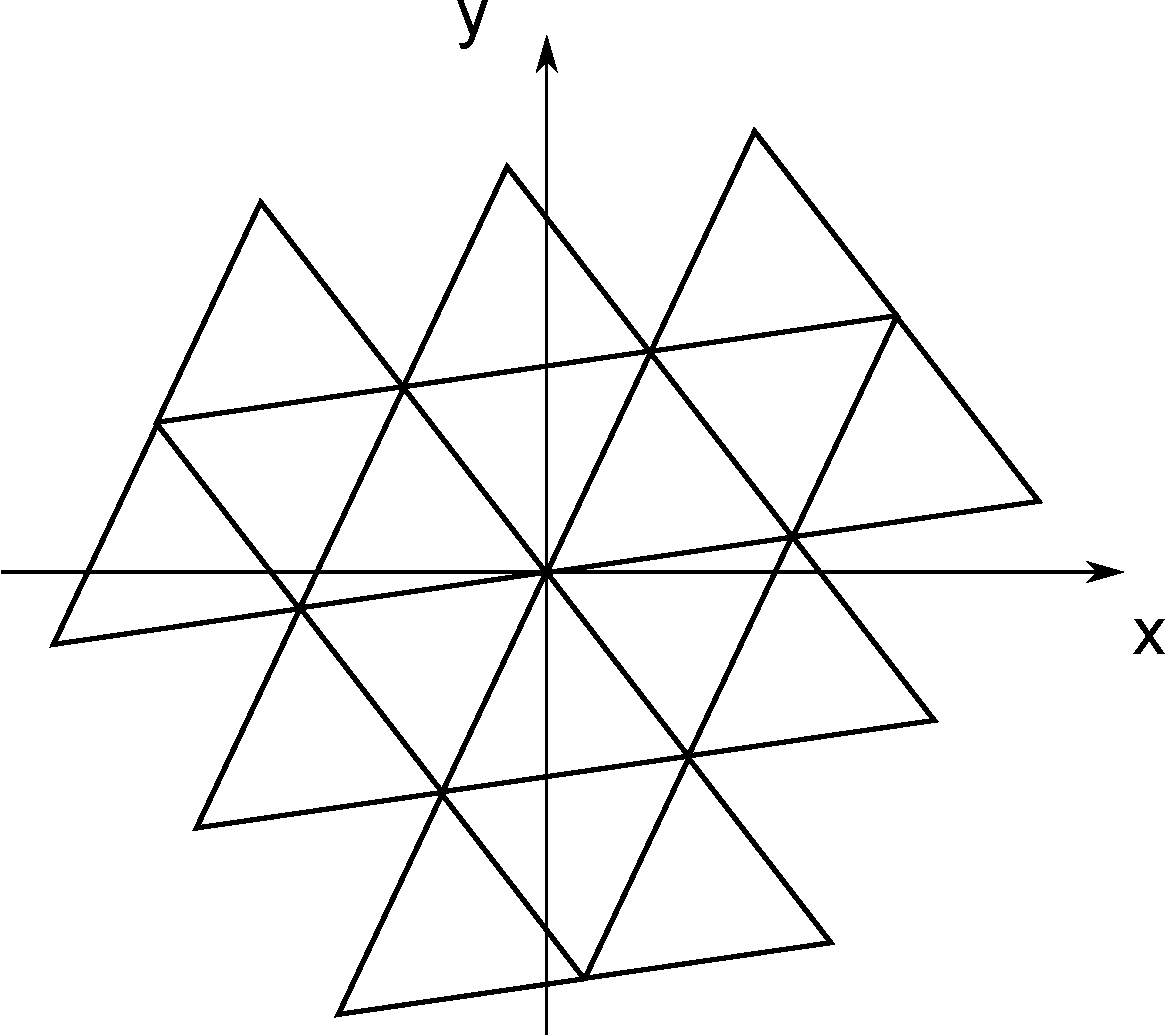
\includegraphics[width=7cm]{simplex_initialfixed.pdf}
\end{center}
\caption{Typical pattern with fixed-shape Spendley's et al algorithm}
\label{fig-nm-simplex-fixedshape}
\end{figure}

The variable-shape simplex algorithm designed by Nelder and Mead is also very
sensitive to the initial simplex.
One of the problems is that the initial simplex should be consistently scaled 
with respect to the unknown $\bx$.
In "An investigation into the efficiency of variants on the simplex method" \cite{parkinson1972}, 
Parkinson and Hutchinson explored 
several improvements of Nelder and Mead's algorithm. First, they investigate the sensitivity
of the algorithm to the initial simplex. Two parameters were investigated,
that is, the initial length and the orientation of the simplex. 
The conclusion of their study with respect to the initial simplex is 
the following. "The orientation of the initial simplex has a significant effect 
on efficiency, but the relationship can be too sensitive for an automatic 
predictor to provide sufficient accuracy at this time."

Since no initial simplex clearly improves on the others, in practice, 
it may be convenient to try different approaches.

\subsection{Spendley's et al regular simplex}

In their paper \cite{Spendley1962}, Spendley et al. use a regular 
simplex with given size $\ell>0$. We define the parameters $p,q>0$ as 
\begin{eqnarray}
p &=& \frac{1}{n\sqrt{2}} \left(n-1 + \sqrt{n+1}\right), \\
q &=& \frac{1}{n\sqrt{2}} \left(\sqrt{n+1} - 1\right).
\end{eqnarray}
We can now define the vertices of the simplex $S=\{\bx_i\}_{i=1,n+1}$.
The first vertex of the simplex is the initial guess 
\begin{eqnarray}
\bv_1 &=& \bx_0.
\end{eqnarray}
The other vertices are defined by 
\begin{eqnarray}
(\bv_i)_j &=& 
\left\{
\begin{array}{l}
(\bx_0)_j + \ell p, \textrm{ if } j=i-1,\\
(\bx_0)_j + \ell q, \textrm{ if } j\neq i-1,\\
\end{array}
\right.
\end{eqnarray}
for vertices $i=2,n+1$ and components $j=1,n$, 
where $\ell \in\RR$ is the length of the simplex and satisfies $\ell>0$. Notice that this 
length is the same for all the edges which keeps the simplex regular.

The regular simplex is presented in figure \ref{fig-nm-simplex-regular}.

\begin{figure}
\begin{center}
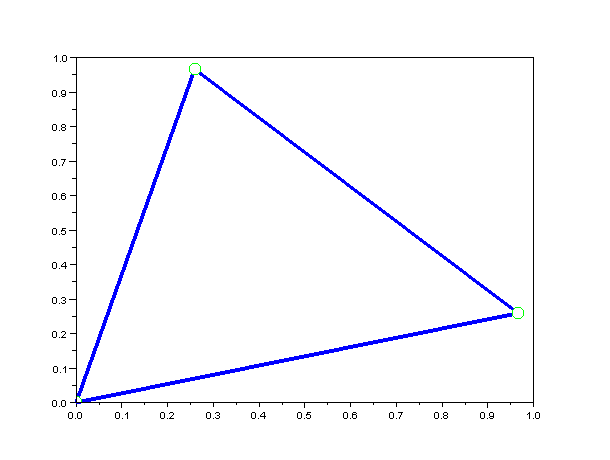
\includegraphics[width=10cm]{simplex_regular.png}
\end{center}
\caption{Regular simplex in 2 dimensions}
\label{fig-nm-simplex-regular}
\end{figure}

\subsection{Axis-by-axis simplex}

A very efficient and simple approach leads to an axis-by-axis simplex.
This simplex depends on a vector of positive lengths $\bl\in\RR^n$.
The first vertex of the simplex is the initial guess 
\begin{eqnarray}
\bv_1 &=& \bx_0.
\end{eqnarray}
The other vertices are defined by 
\begin{eqnarray}
(\bv_i)_j &=& 
\left\{
\begin{array}{l}
(\bx_0)_j + \ell_j, \textrm{ if } j=i-1,\\
(\bx_0)_j, \textrm{ if } j\neq i-1,\\
\end{array}
\right.
\end{eqnarray}
for vertices $i=2,n+1$ and components $j=1,n$.

This type of simplex is presented in figure \ref{fig-nm-simplex-axes},
where $\ell_1=1$ and $\ell_2=2$.
The axis-by-axis simplex is used in the Nelder-Mead 
algorithm provided in Numerical Recipes in C \cite{NumericalRecipes}.
As stated in \cite{NumericalRecipes}, the length vector $\bl$ can 
be used as a guess for the characteristic length scale of the problem.

\begin{figure}
\begin{center}
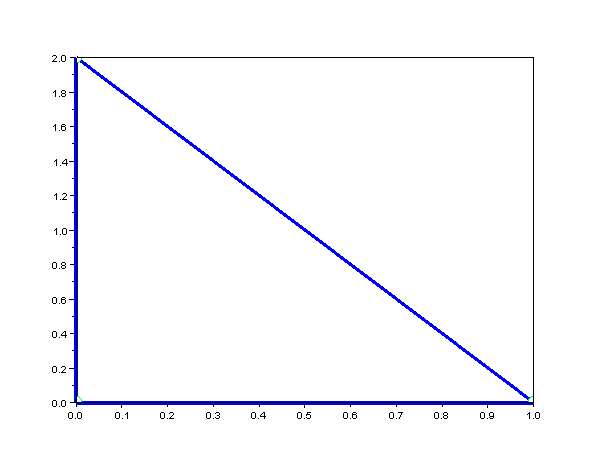
\includegraphics[width=10cm]{simplex_axes.png}
\end{center}
\caption{Axis-based simplex in 2 dimensions -- Notice that the length along the $x$ axis is 1 while the length
along the $y$ axis is 2. }
\label{fig-nm-simplex-axes}
\end{figure}

\subsection{Randomized bounds}

Assume that the variable $\bx\in\RR^n$ is bounded so that 
\begin{eqnarray}
m_j \leq x_j \leq M_j,
\end{eqnarray}
for $j=1,n$, where $m_j,M_j\in\RR$ are minimum 
and maximum bounds and $m_j\leq M_j$.
A method suggested by Box in \cite{Box1965} is 
based on the use of 
pseudo-random numbers. Let 
$\{\theta_{i,j}\}_{i=1,n+1,j=1,n}\in[0,1]$ be 
a sequence of random numbers uniform in the 
interval $[0,1]$.
The first vertex of the simplex is the initial guess 
\begin{eqnarray}
\bv_1 &=& \bx_0.
\end{eqnarray}
The other vertices are defined by 
\begin{eqnarray}
(\bv_i)_j &=& m_j + \theta_{i,j} (M_j - m_j),
\end{eqnarray}
for vertices $i=2,n+1$ and components $j=1,n$.

\subsection{Pfeffer's method}

This initial simplex is used in the function \scifunction{fminsearch}
and presented in \cite{Fan2002}. According to \cite{Fan2002}, this simplex is due to L. Pfeffer at Stanford.
The goal of this method is to scale the initial simplex with respect 
to the characteristic lengths of the problem. This allows, for example,
to manage cases where $x_1\approx 1$ and $x_2\approx 10^5$.
As we are going to see, the scaling is defined with respect to the 
initial guess $\bx_0$, with an axis-by-axis method.

The method proceeds by defining $\delta_u,\delta_z>0$, where 
$\delta_u$ is used for usual components of $\bx_0$ and $\delta_z$ is 
used for the case where one component of $\bx_0$ is zero.
The default values for $\delta_u$ and $\delta_z$ are 
\begin{eqnarray}
\delta_u = 0.05 \qquad \textrm{and} \qquad \delta_z = 0.0075.
\end{eqnarray}
The first vertex of the simplex is the initial guess 
\begin{eqnarray}
\bv_1 &=& \bx_0.
\end{eqnarray}
The other vertices are defined by 
\begin{eqnarray}
(\bv_i)_j &=& \left\{
\begin{array}{l}
(\bx_0)_j + \delta_u (\bx_0)_j, \textrm{ if } j=i-1 \textrm{ and } (\bx_0)_{j-1}\neq 0,\\
\delta_z, \textrm{ if } j=i-1 \textrm{ and } (\bx_0)_{j-1}= 0,\\
(\bx_0)_j, \textrm{ if } j\neq i-1,\\
\end{array}
\right.
\end{eqnarray}
for vertices $i=2,n+1$ and components $j=1,n$.

%\section{The simplex gradient}
%\label{section-simplexgradient}

%TODO...

\section{References and notes}

Some elements of the section \ref{section-simplexsize} is taken from 
Kelley's book \cite{Kelley1999}, "Iterative Methods for Optimization".
While this document focus on Nelder-Mead algorithm, Kelley gives a broad
view on optimization and present other algorithms for noisy functions,
like implicit filtering, multidirectional search and the Hooke-Jeeves algorithm.
\chapter{Spendley's et al. method}

In this chapter, we present Spendley's et al. algorithm \cite{Spendley1962} for 
unconstrained optimization.

We begin by presenting a global overview of the algorithm. 
Then we present various geometric situations which might occur
during the algorithm. In the second section, we present several 
numerical experiments which allow to get some insight in the behavior 
of the algorithm on some simple situations. The two first cases 
are involving only 2 variables and are based on a quadratic function.
The last numerical experiment explores the behavior of the algorithm 
when the number of variables increases.

\section{Introduction}

In this section, we present Spendley's et al algorithm for unconstrained optimization.
This algorithm is based on the iterative update of a simplex. 
At each iteration, either a reflection of a shrink step is performed, so that
the shape of the simplex does not change during the iterations.
Then we present various geometric situations which might occur
during the algorithm. This allows to understand when exactly a reflection 
or a shrink is performed in practice.

\subsection{Overview}

The goal of Spendley's et al. algorithm is to solve the 
following unconstrained optimization problem
\begin{eqnarray}
\min f(\bx)
\end{eqnarray}
where $\bx\in \RR^n$, $n$ is the number of optimization parameters and $f$ is the objective 
function $f:\RR^n\rightarrow \RR$.

This algorithms is based on the iterative update of 
a \emph{simplex} made of $n+1$ points $S=\{\bv_i\}_{i=1,n+1}$. Each point 
in the simplex is called a \emph{vertex} and is associated with 
a function value $f_i=f(\bv_i)$ for $i=1,n+1$.

The vertices are sorted by increasing function values so that the 
\emph{best} vertex has index 1 and the \emph{worst} vertex 
has index $n+1$
\begin{eqnarray}
\label{sp-sorted-vertices-fv}
f_1 \leq f_2 \leq \ldots \leq f_n \leq f_{n+1}.
\end{eqnarray}

The $\bv_1$ vertex (resp. the $\bv_{n+1}$ vertex) is called the \emph{best} 
vertex (resp. \emph{worst}), because it is associated with the lowest (resp. highest)
function value. As we are going to see, the \emph{next-to-worst} vertex $\bv_n$ has a 
special role in this algorithm.

The centroid of the simplex $\overline{\bx} (j)$ is the center of the vertices
where the vertex $\bv_j$ has been 
excluded. This centroid is 
\begin{eqnarray}
\label{sp-centroid-generalized}
\overline{\bx} (j) = \frac{1}{n} \sum_{i=1,n+1, i\neq j} \bv_i.
\end{eqnarray}
The algorithm makes use
of one coefficient $\rho>0$, called the reflection factor. The standard
value of this coefficient is $\rho=1$.
The algorithm attempts to replace some vertex 
$\bv_j$ by a new vertex $\bx(\rho,j)$ on the line from the vertex $\bv_j$
to the centroid  $\overline{\bx}(j)$. The new vertex $\bx(\rho,j)$ is defined by 
\begin{eqnarray}
\label{sp-interpolate-generalized}
\bx(\rho,j) = (1+\rho)\overline{\bx}(j) - \rho \bv_j.
\end{eqnarray}

\subsection{Algorithm}

In this section, we analyze Spendley's et al algorithm, which
is presented in figure \ref{algo-spendley}.

\begin{figure}[htbp]
\begin{algorithmic}
\STATE Compute an initial simplex $S_0$
\STATE Sorts the vertices $S_0$ with increasing function values
\STATE $S\gets S_0$
\WHILE{$\sigma(S)>tol$}
  \STATE $\overline{x}\gets \overline{\bx}(n+1)$ \COMMENT{Compute the centroid}
  \STATE $\bx_r \gets \bx(\rho,n+1)$ \COMMENT{Reflect with respect to worst}
  \STATE $f_r \gets f(\bx_r)$ 
  \IF {$f_r<f_{n+1}$}
    \STATE Accept $\bx_r$
  \ELSE
    \STATE $\overline{x}\gets \overline{\bx}(n)$ \COMMENT{Compute the centroid}
    \STATE $\bx_r^\prime \gets \bx(\rho,n)$ \COMMENT{Reflect with respect to next-to-worst}
    \STATE $f_r^\prime \gets f(\bx_r^\prime)$ 
    \IF {$f_r^\prime<f_{n+1}$}
      \STATE Accept $\bx_r^\prime$
    \ELSE 
      \STATE Compute the vertices $\bv_i=\bv_1 + \sigma (\bv_i - \bv_1)$ for $i=2,n+1$ \COMMENT{Shrink}
      \STATE Compute $f_i = f(\bv_i)$ for $i=2,n+1$
    \ENDIF
  \ENDIF
  \STATE Sort the vertices of $S$ with increasing function values
\ENDWHILE
\end{algorithmic}
\caption{Spendley's et al. algorithm}
\label{algo-spendley}
\end{figure}

At each iteration, we compute the centroid 
$\overline{\bx} (n+1)$ where the worst vertex $\bv_{n+1}$ 
has been excluded. This centroid is 
\begin{eqnarray}
\label{sp-centroid-worst}
\overline{\bx} (n+1) = \frac{1}{n} \sum_{i=1,n} \bv_i.
\end{eqnarray}
We perform a reflection with respect to the worst vertex $\bv_{n+1}$,
which creates the reflected point $\bx_r$ defined by 
\begin{eqnarray}
\label{sp-interpolate-worst}
\bx_r = \bx(\rho,n+1) = (1+\rho)\overline{\bx}(n+1) - \rho \bv_{n+1}
\end{eqnarray}

We then compute the function value of the reflected
point as $f_r=f(\bx_r)$. If the function value $f_r$ is better than the worst function
value $f_{n+1}$, i.e. if $f_r < f_{n+1}$, then the worst vertex $\bv_{n+1}$ is rejected from the 
simplex and the reflected point $\bx_r$ is accepted. If the reflection point 
does not improve the function value $f_{n+1}$, we consider the centroid 
$\overline{\bx} (n)$, i.e. the centroid where the next-to-worst vertex $\bv_n$ has been excluded.
We then consider the reflected point $\bx_r^\prime$, computed from the 
next-to-worst vertex $\bv_n$ and the centroid $\overline{\bx} (n)$. 
We compute the function value $f_r^\prime = f(\bx_r^\prime)$. If the function
value $f_r^\prime$ improves over the worst function value $f_{n+1}$, then 
the worst vertex $\bv_{n+1}$ is rejected from the simplex and the new reflection point 
$\bx_r^\prime$ is accepted.

At that point of the algorithm, neither the reflection with respect to 
$\bv_{n+1}$ nor the reflection with respect to $\bv_n$ were able to improve over 
the worst function value $f_{n+1}$.
Therefore, the algorithm shrinks the simplex toward the best vertex $\bv_1$.
That last step uses the shrink coefficient $0<\sigma<1$. The standard
value for this coefficient is $\sigma=\frac{1}{2}$.

\subsection{Geometric analysis}

The figure \ref{fig-spendley-moves} presents the various 
moves of the Spendley et al. algorithm. It is obvious from the 
picture that the algorithm explores a pattern which is 
entirely determined from the initial simplex.

In Spendley's et al. original paper, the authors use a regular 
simplex, where the edges all have the same length. In practice,
however, any non degenerate simplex can be used.

\begin{figure}
\begin{center}
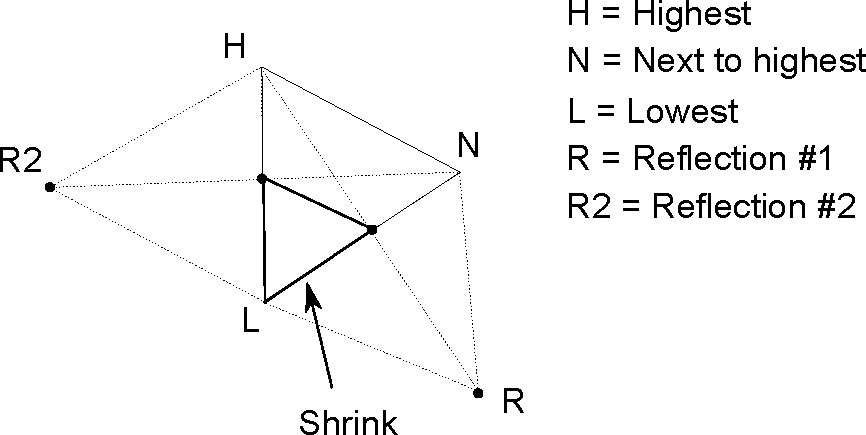
\includegraphics[width=8cm]{spendley-steps.pdf}
\end{center}
\caption{Spendley et al. simplex moves}
\label{fig-spendley-moves}
\end{figure}

The various situations in which these moves are performed are 
presented in figures \ref{fig-spendley-moves-reflect}, \ref{fig-spendley-moves-reflect2}
and \ref{fig-spendley-moves-shrink}.

The basic move is the reflection step, presented in figure 
\ref{fig-spendley-moves-reflect} and \ref{fig-spendley-moves-reflect2}. 
These two figures show that Spendley's et al.
algorithm is based on a discretization of the parameter space. 
The optimum is searched on that grid, which is based on regular simplices.
When no move is possible to improve the situation on that grid,
a shrink step is necessary, as presented in figure \ref{fig-spendley-moves-shrink}.

\begin{figure}
\begin{center}
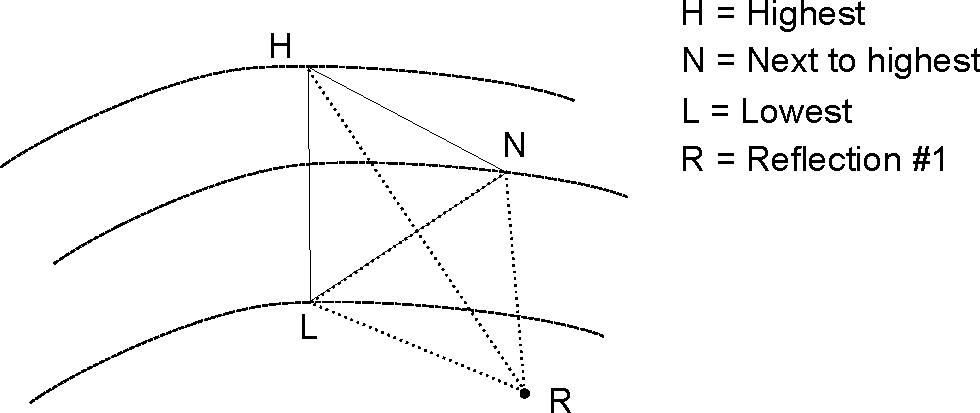
\includegraphics[width=10cm]{spendley-steps-reflect.pdf}
\end{center}
\caption{Spendley et al. simplex moves -- Reflection with respect to highest point}
\label{fig-spendley-moves-reflect}
\end{figure}

\begin{figure}
\begin{center}
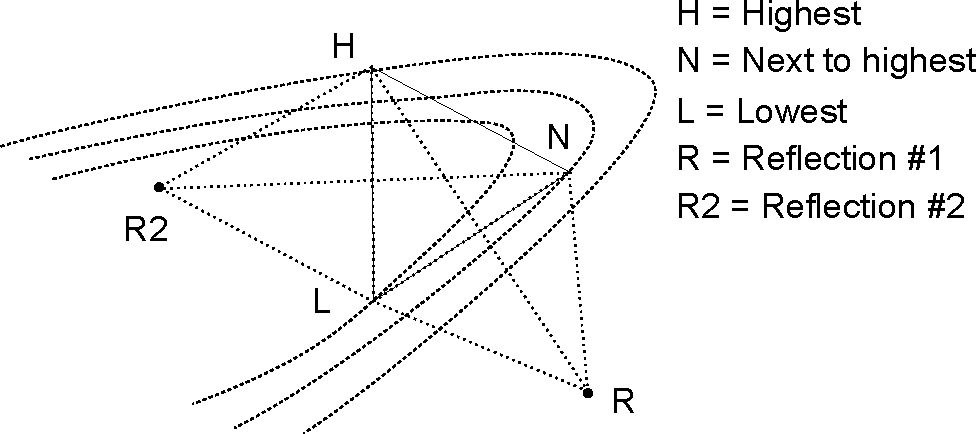
\includegraphics[width=10cm]{spendley-steps-reflect2.pdf}
\end{center}
\caption{Spendley et al. simplex moves -- Reflection with respect to next-to-highest point. 
It may happen that the next iteration is a shrink step.}
\label{fig-spendley-moves-reflect2}
\end{figure}

In the situation of figure \ref{fig-spendley-moves-shrink}, neither the 
reflection \#1 or reflection \#2 have improved the simplex. 
Diminishing the size of the simplex by performing a shrink step 
is the only possible move because the 
simplex has vertices which are located across the valley.
This allows to refine the discretization grid on which the 
optimum is searched.

\begin{figure}
\begin{center}
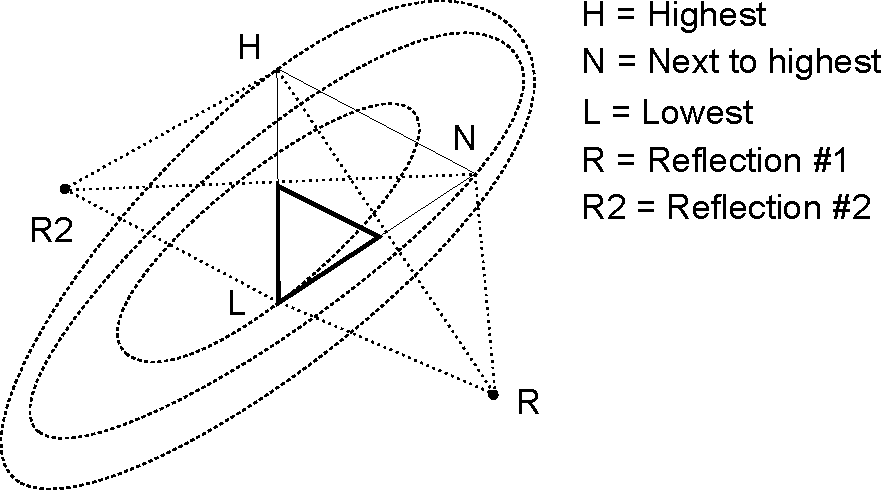
\includegraphics[width=8cm]{spendley-steps-shrink.pdf}
\end{center}
\caption{Spendley et al. simplex moves -- The shrink step is the 
only possible move.}
\label{fig-spendley-moves-shrink}
\end{figure}

%%\subsection{Termination criteria}

%%The original paper \cite{Spendley1962}

\subsection{General features of the algorithm}

From the performance point of viewn when a reflection step is performed,
only 1 or 2 function evaluations are required. Instead, when a shrink
step is performed, there are $n$ function evaluations required. In practice,
reflection steps are performed when the simplex is away from the optimum.
When the simplex is closer to the optimum, or enters in a narrow valley, shrink
steps are used.

As stated in \cite{Singer:2009}, the main feature 
of Spendley's et al. algorithm is that the simplex can vary 
in size, but not in shape. As we are going to see in the numerical 
experiments, this leads to a slow convergence when a narrow 
valley is encountered. In that situation, the shrink
steps are required, which leads to a large number 
of iterations and function evaluations.

In fact, the Spendley's et al. algorithm is a pattern search 
algorithm \cite{Torczon98fromevolutionary}. This is a consequence 
of the fact that the search pattern used in the method is constant.
Therefore, the design never degenerates. 
As stated in \cite{Torczon98fromevolutionary}, "under very mild 
assumptions on $f$, these simple heuristics 
provide enough structure to guarantee global convergence.
This is not the case for the Nelder-Mead algorithm, which might
converge to non-stationnary points \cite{589109, hanNeumann2003, Han2000, Torczon89multi-directionalsearch}. 
In all cases, the difficulty is that a sequence of simplices produced
by the Nelder-Mead simplex method can come arbitrarily close to 
degeneracy.

\section{Numerical experiments}

In this section, we present some numerical experiments 
with Spendley's et al. algorithm.
The first numerical experiments involves one quadratic function
in 2 dimensions. The second experiment is based on a 
badly scaled quadratic in 2 dimension. In the third experiment,
we analyze the behavior of the algorithm with respect to the 
number of variables.

\subsection{Quadratic function}

The function we try to minimize is the following quadratic 
in 2 dimensions 
\begin{eqnarray}
f(x_1,x_2) = x_1^2 + x_2^2 - x_1 x_2.
\end{eqnarray}

The stopping criteria is based on the relative size of the simplex 
with respect to the size of the initial simplex 
\begin{eqnarray}
\sigma_+(S) < tol \times \sigma_+(S_0).
\end{eqnarray}
The oriented length $\sigma_+(S)$ is defined by
\begin{eqnarray}
\sigma_+(S) = \max_{i=2,n+1} \|\bv_i - \bv_1\|_2
\end{eqnarray}
where $\|.\|_2$ is the euclidian norm defined by 
\begin{eqnarray}
\|\bx\|_2 = \sum_{i=1,n}x_i^2.
\end{eqnarray}
In this experiment, we use $tol=10^{-8}$ as the relative tolerance 
on simplex size.

The initial simplex is a regular simplex with length unity.

The following Scilab script performs the optimization.

\lstset{language=scilabscript}
\begin{lstlisting}
function y = quadratic (x)
  y = x(1)^2 + x(2)^2 - x(1) * x(2);
endfunction
nm = neldermead_new ();
nm = neldermead_configure(nm,"-numberofvariables",2);
nm = neldermead_configure(nm,"-function",quadratic);
nm = neldermead_configure(nm,"-x0",[2.0 2.0]');
nm = neldermead_configure(nm,"-maxiter",100);
nm = neldermead_configure(nm,"-maxfunevals",300);
nm = neldermead_configure(nm,"-tolxmethod","disabled");
nm = neldermead_configure(nm,"-tolsimplexizerelative",1.e-8);
nm = neldermead_configure(nm,"-simplex0method","spendley");
nm = neldermead_configure(nm,"-method","fixed");
nm = neldermead_configure(nm,"-verbose",1);
nm = neldermead_configure(nm,"-verbosetermination",0);
nm = neldermead_search(nm);
neldermead_display(nm);
nm = neldermead_destroy(nm);
\end{lstlisting}


The numerical results are presented in table \ref{fig-spendley-numexp1-table}.

\begin{figure}[htbp]
\begin{center}
%\begin{tiny}
\begin{tabular}{|l|l|}
\hline
Iterations & 49 \\
Function Evaluations & 132 \\
$\bx_0$ & $(2.0,2.0)$ \\
Relative tolerance on simplex size & $10^{-8}$ \\
Exact $\bx^\star$ & $(0.,0.)$\\
Computed $\bx^\star$ & $(2.169e-10, 2.169e-10)$\\
Exact $f(\bx^\star)$ & $0.$\\
Computed $f(\bx^\star)$ & $4.706e-20$\\
\hline
\end{tabular}
%\end{tiny}
\end{center}
\caption{Numerical experiment with Spendley's et al. method on the quadratic function
$f(x_1,x_2) = x_1^2 + x_2^2 - x_1 x_2$}
\label{fig-spendley-numexp1-table}
\end{figure}

The various simplices generated during the iterations are 
presented in figure \ref{fig-spendley-numexp1-historysimplex}.
The method use reflections in the early iterations. Then there
is no possible improvement using reflections and shrinking is necessary.
That behavior is an illustration of the discretization which has already
been discussed.

\begin{figure}
\begin{center}
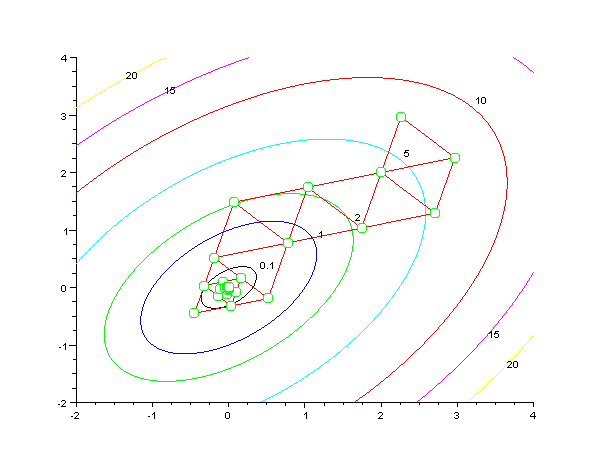
\includegraphics[width=15cm]{quad2bis-spendley-simplexcontours.png}
\end{center}
\caption{Spendley et al. numerical experiment -- History of simplex}
\label{fig-spendley-numexp1-historysimplex}
\end{figure}

The figure \ref{fig-spendley-numexp1-sigma} presents the history of the oriented
length of the simplex. The length is updated step by step, where each step 
corresponds to a shrink in the algorithm.

\begin{figure}
\begin{center}
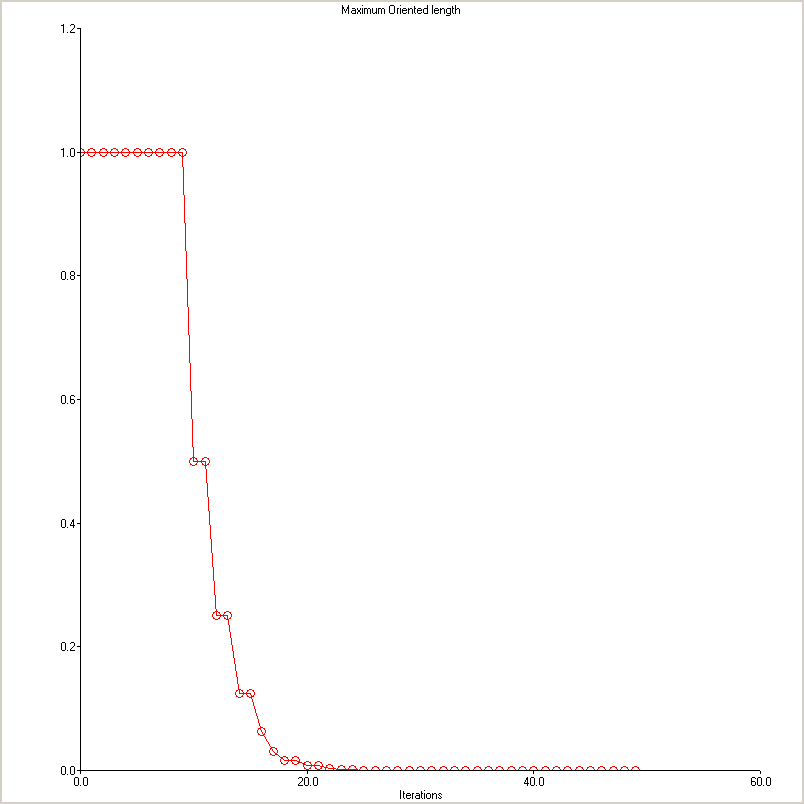
\includegraphics[width=10cm]{quad2bis-spendley-history-sigma.png}
\end{center}
\caption{Spendley et al. numerical experiment -- History of logarithm of the size of the simplex}
\label{fig-spendley-numexp1-sigma}
\end{figure}

The convergence is quite fast in this case, since less than 60 iterations
allow to get a function value lower than $10^{-15}$, as shown in 
figure \ref{fig-spendley-numexp1-logfopt}.

\begin{figure}
\begin{center}
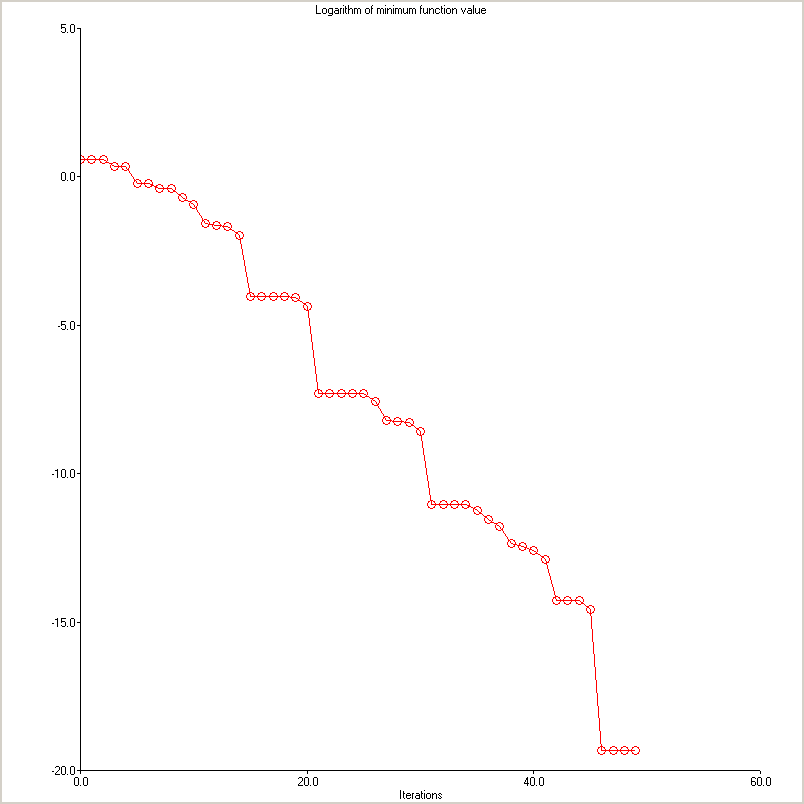
\includegraphics[width=10cm]{quad2bis-spendley-history-logfopt.png}
\end{center}
\caption{Spendley et al. numerical experiment -- History of logarithm of function}
\label{fig-spendley-numexp1-logfopt}
\end{figure}

\subsection{Badly scaled quadratic function}

The function we try to minimize is the following quadratic 
in 2 dimensions 
\begin{eqnarray}
\label{quadratic-sp-function2}
f(x_1,x_2) = a x_1^2 + x_2^2,
\end{eqnarray}
where $a>0$ is a chosen scaling parameter. 
The more $a$ is large, the more difficult the problem is 
to solve with the simplex algorithm.
Indeed, let us compute the Hessian matrix associated with the 
cost function. We have 
\begin{eqnarray}
\bH = \left(
\begin{array}{cc}
2 a & 0 \\
0 & 2
\end{array}
\right).
\end{eqnarray}
Therefore, the eigenvalues of the Hessian matrix 
are $2a$ and $2$, which are stricly 
positive if $a>0$. Hence, the cost function is stricly convex and 
there is only one global solution, that is $\bx^\star = (0,0,\ldots,0)^T$.
The ratio between these two eigenvalues is $a$. This leads 
to an elongated valley, which is extremely narrow when $a$ is large.

The stopping criteria is based on the relative size of the simplex 
with respect to the size of the initial simplex 
\begin{eqnarray}
\sigma_+(S) < tol \times \sigma_+(S_0).
\end{eqnarray}
In this experiment, we use $tol=10^{-8}$ as the relative tolerance 
on simplex size.

We set the maximum number of function evaluations to 400.
The initial simplex is a regular simplex with length unity.

The following Scilab script uses the neldermead algorithm to perform the 
optimization.

\lstset{language=scilabscript}
\begin{lstlisting}
a = 100;
function y = quadratic (x)
  y = a * x(1)^2 + x(2)^2;
endfunction
nm = nmplot_new ();
nm = nmplot_configure(nm,"-numberofvariables",2);
nm = nmplot_configure(nm,"-function",quadratic);
nm = nmplot_configure(nm,"-x0",[10.0 10.0]');
nm = nmplot_configure(nm,"-maxiter",400);
nm = nmplot_configure(nm,"-maxfunevals",400);
nm = nmplot_configure(nm,"-tolxmethod","disabled");
nm = nmplot_configure(nm,"-tolsimplexizerelative",1.e-8);
nm = nmplot_configure(nm,"-simplex0method","spendley");
nm = nmplot_configure(nm,"-method","fixed");
nm = nmplot_configure(nm,"-verbose",1);
nm = nmplot_configure(nm,"-verbosetermination",0);
nm = nmplot_configure(nm,"-simplexfn","rosenbrock.fixed.history.simplex.txt");
nm = nmplot_configure(nm,"-fbarfn","rosenbrock.fixed.history.fbar.txt");
nm = nmplot_configure(nm,"-foptfn","rosenbrock.fixed.history.fopt.txt");
nm = nmplot_configure(nm,"-sigmafn","rosenbrock.fixed.history.sigma.txt");
nm = nmplot_search(nm);
nmplot_display(nm);
nm = nmplot_destroy(nm);
\end{lstlisting}


The numerical results are presented in table \ref{fig-spendley-numexp1-table},
where the experiment is presented for $a=100$. We can check that the 
number of function evaluations is equal to its maximum limit, even if the value of the 
function at optimum is very inaccurate ($f(\bx^\star) \approx 0.08$).

\begin{figure}[h]
\begin{center}
%\begin{tiny}
\begin{tabular}{|l|l|}
\hline
Iterations & 340 \\
Function Evaluations & 400 \\
$a$ & $100.0$ \\
$\bx_0$ & $(10.0,10.0)$ \\
Relative tolerance on simplex size & $10^{-8}$ \\
Exact $\bx^\star$ & $(0.,0.)$\\
Computed $\bx^\star$ & $(0.001,0.2)$\\
Computed $f(\bx^\star)$ & $0.08$\\
\hline
\end{tabular}
%\end{tiny}
\end{center}
\caption{Numerical experiment with Spendley's et al. method on a badly scaled quadratic function}
\label{fig-spendley-numexp2-table}
\end{figure}

The various simplices generated during the iterations are 
presented in figure \ref{fig-spendley-numexp2-historysimplex}.
The method use reflections in the early iterations. Then there
is no possible improvement using reflections, so that shrinking is necessary.
But the repeated shrink steps makes the simplex very small, leading to a large number of 
iterations. This is a limitation of the method, which is based on a simplex 
which can vary its size, but not its shape.

\begin{figure}
\begin{center}
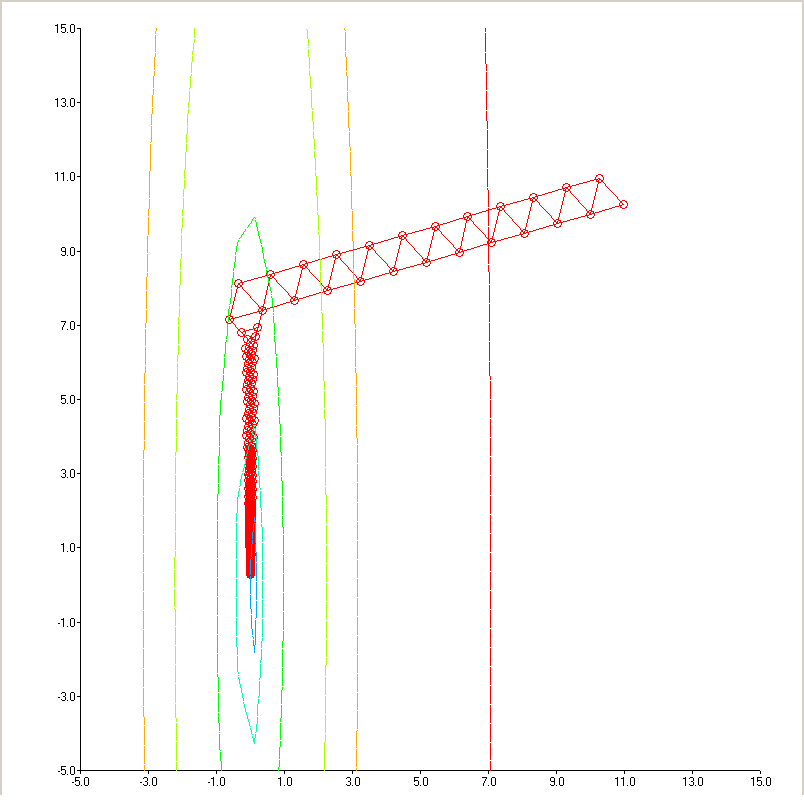
\includegraphics[width=15cm]{quad2-spendley-simplexcontours.png}
\end{center}
\caption{Spendley et al. numerical experiment with $f(x_1,x_2) = a x_1^2 + x_2^2$ and $a=100$ -- History of simplex}
\label{fig-spendley-numexp2-historysimplex}
\end{figure}

In figure \ref{fig-spendley-numexp2-scaling}, we analyze the 
behavior of the method with respect to scaling.
We check that the method behave poorly when the scaling is 
bad. The convergence speed is slower and slower and impractical 
when $a>10$

\begin{figure}[htbp]
\begin{center}
%\begin{tiny}
\begin{tabular}{|l|l|l|}
\hline
$a$ & Function evaluations & Computed $f(\bx^\star)$ \\
$1.0$ & 160 & $2.35e-18$ \\
$10.0$ & 222 & $1.2e-17$ \\
$100.0$ & 400 & $0.083$ \\
$1000.0$ & 400 & $30.3$ \\
$10000.0$ & 400 & $56.08$ \\
\hline
\end{tabular}
%\end{tiny}
\end{center}
\caption{Numerical experiment with Spendley's et al. method on a badly scaled quadratic function}
\label{fig-spendley-numexp2-scaling}
\end{figure}

\subsection{Sensitivity to dimension}

In this section, we try to study the convergence of the 
Spendley et al. algorithm with respect to the number of variables,
as presented by Han \& Neumann in \cite{HanNeumann2006}.
We emphasize, though, that Han \& Neumann present their numerical 
experiment with the Nelder-Mead algorithm, while we present 
in this section the Spendley et al. algorithm.
The function we try to minimize is the following quadratic function 
in $n$-dimensions 
\begin{eqnarray}
\label{quadratic-sp-function3}
f(\bx) = \sum_{i=1,n} x_i^2.
\end{eqnarray}

The initial guess is the origin $\bx_0 = (0,0,\ldots,0)^T$,
which is also the global solution of the problem.
We have $f(\bx_0)=0$ so that this vertex is never updated 
during the iterations.
The initial simplex is computed with a random number generator.
The first vertex of the initial simplex is the origin.
The other vertices are uniform in the $[-1,1]$ interval.
An absolute termination criteria on the size of the simplex is used, 
that is, the algorithm is stopped when the inequality 
$\sigma_+(S_k) \leq 10^{-8}$ is satisfied.

For this test, we compute the rate of convergence as presented
in Han \& Neuman \cite{HanNeumann2006}. This rate is defined as 
\begin{eqnarray}
\label{rho-sp-rate-convergence}
\rho(S_0,n) = \textrm{lim sup}_{k\rightarrow \infty} 
\left(\prod_{i=0,k-1} \frac{\sigma(S_{i+1})}{\sigma(S_i)}\right)^{1/k},
\end{eqnarray}
where $k$ is the number of iterations.
That definition can be viewed as the geometric mean of the ratio of the 
oriented lengths between successive simplices.
This definition implies 
\begin{eqnarray}
\label{rho-sp-rate-convergence2}
\rho(S_0,n) = \textrm{lim sup}_{k\rightarrow \infty} 
\left(\frac{\sigma(S_k)}{\sigma(S_0)}\right)^{1/k},
\end{eqnarray}

If $k$ is the number of iterations required to obtain convergence, as 
indicated by the termination criteria, the rate of convergence is practically computed as 
\begin{eqnarray}
\rho(S_0,n,k) = \left( \frac{\sigma(S_{k})}{\sigma(S_0)}\right)^{1/k}.
\end{eqnarray}

The following Scilab script allows to perform the optimization.

\lstset{language=scilabscript}
\begin{lstlisting}
function y = quadratic (x)
  y = x(:).' * x(:);
endfunction
//
// myoutputcmd --
//  This command is called back by the Nelder-Mead
//  algorithm.
// Arguments
//  state : the current state of the algorithm
//    "init", "iter", "done"
//  data : the data at the current state
//    This is a tlist with the following entries:
//    * x : the optimal vector of parameters
//    * fval : the minimum function value
//    * simplex : the simplex, as a simplex object
//    * iteration : the number of iterations performed
//    * funccount : the number of function evaluations
//    * step : the type of step in the previous iteration
//
function myoutputcmd ( state , data , step )
  global STEP_COUNTER
  STEP_COUNTER(step) = STEP_COUNTER(step) + 1
endfunction

// OptimizeHanNeumann --
//   Perform the optimization and returns the object
// Arguments 
//   N : the dimension
function nm = OptimizeHanNeumann ( N )
  global STEP_COUNTER
  STEP_COUNTER("init") = 0;
  STEP_COUNTER("done") = 0;
  STEP_COUNTER("reflection") = 0;
  STEP_COUNTER("expansion") = 0;
  STEP_COUNTER("insidecontraction") = 0;
  STEP_COUNTER("outsidecontraction") = 0;
  STEP_COUNTER("expansion") = 0;
  STEP_COUNTER("shrink") = 0;
  STEP_COUNTER("reflectionnext") = 0;

  x0 = zeros(N,1);
  nm = neldermead_new ();
  nm = neldermead_configure(nm,"-numberofvariables",N);
  nm = neldermead_configure(nm,"-function",quadratic);
  nm = neldermead_configure(nm,"-x0",x0);
  nm = neldermead_configure(nm,"-maxiter",10000);
  nm = neldermead_configure(nm,"-maxfunevals",10000);
  nm = neldermead_configure(nm,"-tolxmethod","disabled");
  nm = neldermead_configure(nm,"-tolsimplexizeabsolute",1.e-8);
  nm = neldermead_configure(nm,"-tolsimplexizerelative",0);
  nm = neldermead_configure(nm,"-simplex0method","given");
  coords0(1,1:N) = zeros(1,N);
  coords0(2:N+1,1:N) = 2 * rand(N,N) - 1;
  nm = neldermead_configure(nm,"-coords0",coords0);
  nm = neldermead_configure(nm,"-method","fixed");
  nm = neldermead_configure(nm,"-verbose",0);
  nm = neldermead_configure(nm,"-verbosetermination",0);
  nm = neldermead_configure(nm,"-outputcommand",myoutputcmd);
  //
  // Perform optimization
  //
  nm = neldermead_search(nm);
endfunction

for N = 1:10
  nm = OptimizeHanNeumann ( N );
  niter = neldermead_get ( nm , "-iterations" );
  funevals = neldermead_get ( nm , "-funevals" );
  simplex0 = neldermead_get ( nm , "-simplex0" );
  sigma0 = optimsimplex_size ( simplex0 , "sigmaplus" );
  simplexopt = neldermead_get ( nm , "-simplexopt" );
  sigmaopt = optimsimplex_size ( simplexopt , "sigmaplus" );
  rho = ( sigmaopt / sigma0 ) ^ ( 1 / niter );
  //mprintf ( "%d %d %d %e\n" , N , funevals , niter , rho );
  mprintf("%d %s\n",N, strcat(string(STEP_COUNTER)," "))
  nm = neldermead_destroy(nm);
end

\end{lstlisting}

The figure \ref{fig-sp-numexp3-nbsteps} presents the type of 
steps which are performed for each number of variables.
We see that the algorithm mostly performs shrink steps.

\begin{figure}[htbp]
\begin{center}
%\begin{tiny}
\begin{tabular}{|l|l|l|l|l|}
\hline
$n$ & \#Iterations & \# Reflections & \# Reflection & \#Shrink\\
 & & / High & / Next to High & \\
\hline
1 & 27 & 0 & 0 & 26\\
2 & 28 & 0 & 0 & 27\\
3 & 30 & 2 & 0 & 27\\
4 & 31 & 1 & 1 & 28\\
5 & 29 & 0 & 0 & 28\\
6 & 31 & 2 & 0 & 28\\
7 & 29 & 0 & 0 & 28\\
8 & 29 & 0 & 0 & 28\\
9 & 29 & 0 & 0 & 28\\
10 & 29 & 0 & 0 & 28\\
11 & 29 & 0 & 0 & 28\\
12 & 29 & 0 & 0 & 28\\
13 & 31 & 0 & 2 & 28\\
14 & 29 & 0 & 0 & 28\\
15 & 29 & 0 & 0 & 28\\
16 & 31 & 0 & 1 & 29\\
17 & 30 & 0 & 0 & 29\\
18 & 30 & 0 & 0 & 29\\
19 & 31 & 0 & 1 & 29\\
20 & 32 & 2 & 0 & 29\\
\hline
\end{tabular}
%\end{tiny}
\end{center}
\caption{Numerical experiment with Spendley et al method on a 
generalized quadratic function -- Number of iterations 
and types of steps performed}
\label{fig-sp-numexp3-nbsteps}
\end{figure}

The figure \ref{fig-sp-numexp3-dimension} presents the number of function 
evaluations depending on the number of variables.
We can see that the number of function evaluations 
increases approximately linearly with the dimension of the problem in
figure \ref{fig-sp-numexp3-fvn}. A rough rule of thumb is that, for $n=1,20$, 
the number of function evaluations is equal to $30n$:
most iterations are shrink steps and approximately 30 iterations are required,
almost independently of $n$.

\begin{figure}[htbp]
\begin{center}
%\begin{tiny}
\begin{tabular}{|l|l|l|l|}
\hline
$n$ & Function  & Iterations & $\rho(S_0,n)$\\
    & Evaluations &          & \\
\hline
1 & 81 & 27 & 0.513002 \\
2 & 112 & 28 & 0.512532 \\
3 & 142 & 29 & 0.524482 \\
4 & 168 & 28 & 0.512532 \\
5 & 206 & 31 & 0.534545 \\
6 & 232 & 29 & 0.512095 \\
7 & 262 & 30 & 0.523127 \\
8 & 292 & 30 & 0.523647 \\
9 & 321 & 30 & 0.523647 \\
10 & 348 & 29 & 0.512095 \\
11 & 377 & 29 & 0.512095 \\
12 & 406 & 29 & 0.512095 \\
13 & 435 & 29 & 0.512095 \\
14 & 464 & 29 & 0.512095 \\
15 & 493 & 29 & 0.512095 \\
16 & 540 & 30 & 0.511687 \\
17 & 570 & 30 & 0.511687 \\
18 & 600 & 30 & 0.511687 \\
19 & 630 & 30 & 0.511687 \\
20 & 660 & 30 & 0.511687 \\
\hline
\end{tabular}
%\end{tiny}
\end{center}
\caption{Numerical experiment with Spendley et al. method on a generalized quadratic function}
\label{fig-sp-numexp3-dimension}
\end{figure}

\begin{figure}
\begin{center}
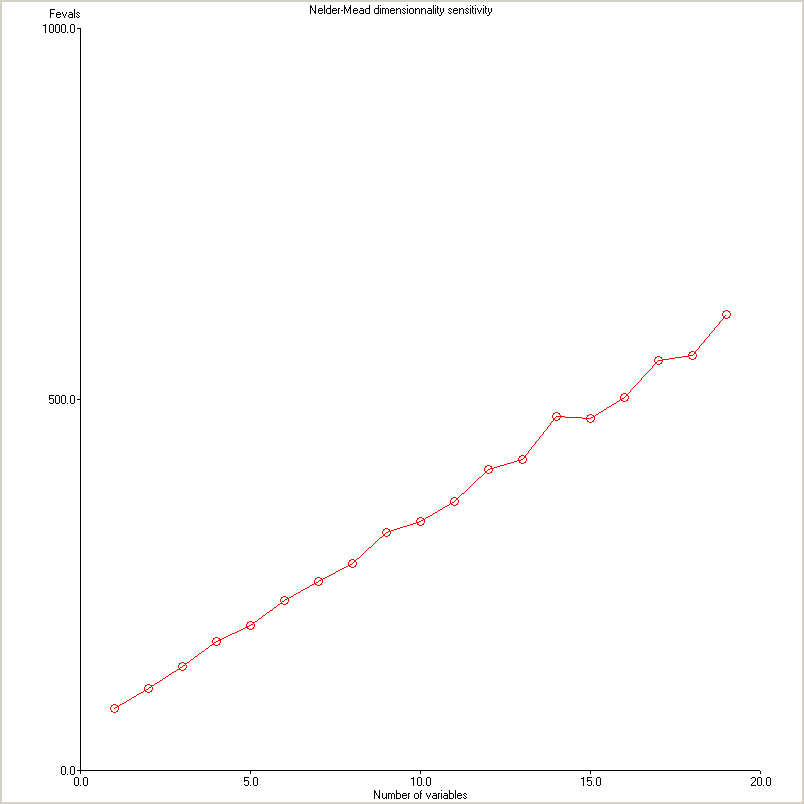
\includegraphics[width=10cm]{spendley-dimension-nfevals.png}
\end{center}
\caption{Spendley et al. numerical experiment -- Number of function evaluations 
depending on the number of variables}
\label{fig-sp-numexp3-fvn}
\end{figure}

The table \ref{fig-sp-numexp3-dimension} also shows the interesting 
fact that the convergence rate is almost constant and 
very close to $1/2$. This is a consequence of the shrink steps,
which are dividing the size of the simplex at each iteration by 2.

\section{Conclusion}

We saw in the first numerical experiment that the method 
behave reasonably when the function is correctly scaled.
When the function is badly scaled, as in the second numerical 
experiment, the Spendley et al. algorithm produces a large 
number of function evaluations and converges very slowly.
This limitation occurs with even moderate badly scaled 
functions and generates a very slow method in these 
cases.

In the last experiment, we have explored what happens when the number of 
iterations is increasing. In this experiment, the rate of convergence is close to $1/2$
and the number of function evaluations is a linear function of the number 
of variables (approximately $30n$).


\chapter{Nelder-Mead method}

In this chapter, we present Nelder and Mead's \cite{citeulike:3009487} algorithm.
We begin by the analysis of the algorithm, which is based on a variable shape simplex.
Then, we present geometric situations where the various steps of the algorithm 
are used. In the third part, we present the rate of convergence toward the optimum of 
the Nelder-Mead algorithm. This part is mainly based on Han and Neumann's paper \cite{HanNeumann2006}, 
which makes use of a class of quadratic functions with a special initial 
simplex. The core of this chapter is the analysis of several numerical 
experiments which have been performed with the neldermead component.
We analyze the behavior of the algorithm on quadratic functions and 
present several counter examples where the Nelder-Mead algorithm is 
known to fail.

\section{Introduction}

In this section, we present the Nelder-Mead algorithm for unconstrained optimization.
This algorithm is based on the iterative update of a simplex. 
Then we present various geometric situations which might occur
during the algorithm. 

\subsection{Overview}

The goal of the Nelder and Mead algorithm is to solve the 
following unconstrained optimization problem
\begin{eqnarray}
\min f(\bx)
\end{eqnarray}
where $\bx\in \RR^n$, $n$ is the number of optimization parameters and $f$ is the objective 
function $f:\RR^n\rightarrow \RR$.

The Nelder-Mead method is an improvement over the Spendley's et al.
method with the goal of allowing the simplex to vary in \emph{shape}, 
and not only in \emph{size}, as in Spendley's et al. algorithm.

This algorithms is based on the iterative update of 
a \emph{simplex} made of $n+1$ points $S=\{\bv_i\}_{i=1,n+1}$. Each point 
in the simplex is called a \emph{vertex} and is associated with 
a function value $f_i=f(\bv_i)$ for $i=1,n+1$.

The vertices are sorted by increasing function values so that the 
\emph{best} vertex has index 1 and the \emph{worst} vertex 
has index $n+1$
\begin{eqnarray}
\label{sorted-vertices-fv}
f_1 \leq f_2 \leq \ldots \leq f_n \leq f_{n+1}.
\end{eqnarray}

The $\bv_1$ vertex (resp. the $\bv_{n+1}$ vertex) is called the \emph{best} 
vertex (resp. \emph{worst}), because it is associated with the lowest (resp. highest)
function value. 

The centroid of the simplex $\overline{\bx} (j)$ is the center of the vertices
where the vertex $\bv_j$ has been 
excluded. This centroid is 
\begin{eqnarray}
\label{centroid-generalized}
\overline{\bx} (j) = 
\frac{1}{n} \sum_{i=1,n+1, i\neq j} \bv_i.
\end{eqnarray}
The algorithm makes use
of one coefficient $\rho>0$, called the reflection factor. The standard
value of this coefficient is $\rho=1$.
The algorithm attempts to replace some vertex 
$\bv_j$ by a new vertex $\bx(\rho,j)$ on the line from the vertex $\bv_j$
to the centroid  $\overline{\bx}(j)$. The new vertex $\bx(\rho,j)$ is defined by 
\begin{eqnarray}
\label{interpolate-generalized}
\bx(\rho,j) = (1+\rho)\overline{\bx}(j) - \rho \bv_j.
\end{eqnarray}

\subsection{Algorithm}

In this section, we analyze the Nelder-Mead algorithm, which
is presented in figure \ref{algo-neldermead}.

\begin{figure}[htbp]
\begin{algorithmic}
\STATE Compute an initial simplex $S_0$
\STATE Sorts the vertices $S_0$ with increasing function values
\STATE $S\gets S_0$
\WHILE{$\sigma(S)>tol$}
  \STATE $\overline{x}\gets \overline{x}(n+1)$
  \STATE $x_r \gets x(\rho,n+1)$ \COMMENT{Reflect}
  \STATE $f_r \gets f(x_r)$ 
  \IF {$f_r<f_1$}
    \STATE $x_e \gets x(\rho\chi,n+1)$ \COMMENT{Expand}
    \STATE $f_e \gets f(x_e)$ 
    \IF {$f_e<f_r$}
      \STATE Accept $x_e$
    \ELSE
      \STATE Accept $x_r$
    \ENDIF
  \ELSIF {$f_1 \leq f_r < f_n$}
    \STATE Accept $x_r$
  \ELSIF {$f_n \leq f_r < f_{n+1}$}
    \STATE $x_c \gets x(\rho\gamma,n+1)$ \COMMENT{Outside contraction}
    \STATE $f_c \gets f(x_c)$ 
    \IF {$f_c<f_r$}
      \STATE Accept $x_c$
    \ELSE
      \STATE Compute the points $x_i=x_1 + \sigma (x_i - x_1)$, $i=2,n+1$ \COMMENT{Shrink}
      \STATE Compute $f_i = f(\bv_i)$ for $i=2,n+1$
    \ENDIF
  \ELSE
    \STATE $x_c \gets x(-\gamma,n+1)$ \COMMENT{Inside contraction}
    \STATE $f_c \gets f(x_c)$ 
    \IF {$f_c<f_{n+1}$}
      \STATE Accept $x_c$
    \ELSE
      \STATE Compute the points $x_i=x_1 + \sigma (x_i - x_1)$, $i=2,n+1$ \COMMENT{Shrink}
      \STATE Compute $f_i = f(\bv_i)$ for $i=2,n+1$
    \ENDIF
  \ENDIF
  \STATE Sort the vertices of $S$ with increasing function values
\ENDWHILE
\end{algorithmic}
\caption{Nelder-Mead algorithm -- Standard version}
\label{algo-neldermead}
\end{figure}

The Nelder-Mead algorithm makes use of four parameters: the 
coefficient of reflection $\rho$, expansion $\chi$, 
contraction $\gamma$ and shrinkage $\sigma$.
When the expansion or contraction steps are performed, the shape 
of the simplex is changed, thus "adapting itself to the 
local landscape" \cite{citeulike:3009487}.

These parameters should satisfy the following inequalities \cite{citeulike:3009487,lagarias:112}
\begin{eqnarray}
\label{condition-coeffs}
\rho>0, \qquad \chi > 1, \qquad \chi > \rho, \qquad 0<\gamma<1 \qquad \textrm{and} \qquad 0<\sigma<1.
\end{eqnarray}
The standard values for these coefficients are 
\begin{eqnarray}
\label{standard-coeffs}
\rho=1, \qquad \chi =2, \qquad \gamma=\frac{1}{2} \qquad \textrm{and} \qquad \sigma=\frac{1}{2}.
\end{eqnarray}

In \cite{Kelley1999}, the Nelder-Mead algorithm is presented with 
other parameter names, that is $\mu_r = \rho$, $\mu_e = \rho\chi$, $\mu_{ic} = -\gamma$
and $\mu_{oc} = \rho\gamma$. These coefficients must satisfy the following 
inequality 
\begin{eqnarray}
-1 < \mu_{ic} < 0 < \mu_{oc} < \mu_r < \mu_e.
\end{eqnarray}

At each iteration, we compute the centroid 
$\overline{\bx} (n+1)$ where the worst vertex $\bv_{n+1}$ 
has been excluded. This centroid is 
\begin{eqnarray}
\label{centroid-worst}
\overline{\bx} (n+1) = \frac{1}{n} \sum_{i=1,n} \bv_i.
\end{eqnarray}
We perform a reflection with respect to the worst vertex $\bv_{n+1}$,
which creates the reflected point $\bx_r$ defined by 
\begin{eqnarray}
\label{interpolate-worst}
\bx_r = \bx(\rho,n+1) = (1+\rho)\overline{\bx}(n+1) - \rho \bv_{n+1}
\end{eqnarray}
We then compute the function value of the reflected
point as $f_r=f(\bx_r)$. 

From that point, there are several possibilities, which 
are listed below. Most steps try to replace the 
worst vertex $\bv_{n+1}$ by a better point, which is computed 
depending on the context.
\begin{itemize}
\item In the case where $f_r<f_1$, the reflected point $\bx_r$
were able to improve (i.e. reduce) the function value. In that case, the algorithm
tries to expand the simplex so that the function value is improved 
even more. The expansion point is computed by 
\begin{eqnarray}
\bx_e = \bx(\rho\chi,n+1) = (1+\rho\chi)\overline{\bx}(n+1) - \rho\chi \bv_{n+1}
\end{eqnarray}
and the function is computed at this point, i.e. we compute 
$f_e = f(\bx_e)$.
If the expansion point allows to improve the function 
value, the worst vertex 
$\bv_{n+1}$ is rejected from the simplex and the expansion point $\bx_e$
is accepted. If not, the reflection point $\bx_r$ is accepted.
\item In the case where $f_1\leq f_r<f_n$, the worst vertex 
$\bv_{n+1}$ is rejected from the simplex and the reflected point $\bx_r$
is accepted.
\item In the case where $f_n\leq f_r<f_{n+1}$, we consider the point 
\begin{eqnarray}
\bx_c = \bx(\rho\gamma,n+1) = (1+\rho\gamma)\overline{\bx}(n+1) - \rho\gamma \bv_{n+1}
\end{eqnarray}
is considered. If the point $\bx_c$ is better than the reflection point $\bx_r$,
then it is accepted. If not, a shrink step is performed, where 
all vertices are moved toward the best vertex $\bv_1$.
\item In other cases, we consider the point 
\begin{eqnarray}
\bx_c = \bx(-\gamma,n+1) = (1-\gamma)\overline{\bx}(n+1) + \gamma \bv_{n+1}.
\end{eqnarray}
If the point $\bx_c$ is better than the worst vertex $\bx_{n+1}$,
then it is accepted. If not, a shrink step is performed.
\end{itemize}

The algorithm from figure \ref{algo-neldermead} is the most 
popular variant of the Nelder-Mead algorithm.
But the original paper is based on a "greedy" expansion, where 
the expansion point is accepted if it is better than the 
best point (and not if it is better than the reflection point).
This "greedy" version is implemented in AS47 by O'Neill in \cite{O'Neill1971AAF}
and the corresponding algorithm is presented in figure \ref{algo-neldermead-greedy}.

\begin{figure}[htbp]
\begin{verbatim}
[...]
\end{verbatim}
\begin{algorithmic}
    \STATE $\bx_e \gets \bx(\rho\chi,n+1)$ \COMMENT{Expand}
    \STATE $f_e \gets f(\bx_e)$ 
    \IF {$f_e<f_1$}
      \STATE Accept $\bx_e$
    \ELSE
      \STATE Accept $\bx_r$
    \ENDIF
\end{algorithmic}
\begin{verbatim}
[...]
\end{verbatim}
\caption{Nelder-Mead algorithm -- Greedy version}
\label{algo-neldermead-greedy}
\end{figure}


\section{Geometric analysis}

The figure \ref{fig-nm-moves} presents the various moves of the 
simplex in the Nelder-Mead algorithm.

\begin{figure}
\begin{center}
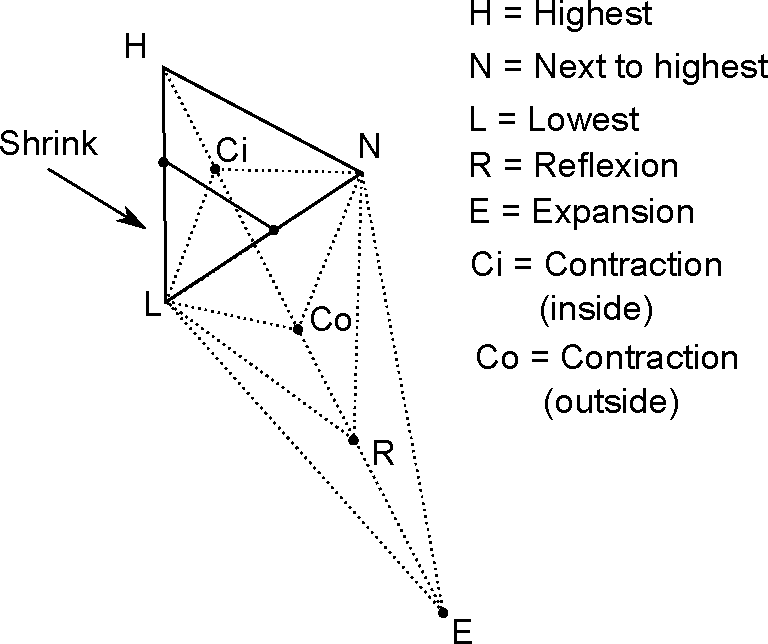
\includegraphics[width=6cm]{nelder-mead-steps.pdf}
\end{center}
\caption{Nelder-Mead simplex steps}
\label{fig-nm-moves}
\end{figure}

The figure \ref{fig-nm-moves-reflection} 
to \ref{fig-nm-moves-shrinkafterco} present the 
detailed situations when each type of step occur.
We emphasize that these figures are not the result of 
numerical experiments. These figures been created in order 
to illustrate specific points of the algorithm.

\begin{itemize}
\item Obviously, the expansion step is performed when the 
simplex is far away from the optimum. The direction of 
descent is then followed and the worst vertex is moved 
into that direction.
\item When the reflection step is performed, the simplex is 
getting close to an valley, since the expansion point 
does not improve the function value.
\item When the simplex is near the optimum, 
the inside and outside contraction steps may be performed, which 
allows to decrease the size of the simplex.
The figure \ref{fig-nm-moves-insidecontraction}, which illustrates 
the inside contraction step, happens in "good" situations.
As presented in section \ref{section-mcKinnon}, applying 
repeatedly the inside contraction step can transform 
the simplex into a degenerate simplex, which may let the algorithm
converge to a non stationnary point.
\item The shrink steps (be it after an outside contraction or an inside 
contraction) occurs only in very special situations. In practical experiments,
shrink steps are rare.
\end{itemize}

\begin{figure}
\begin{center}
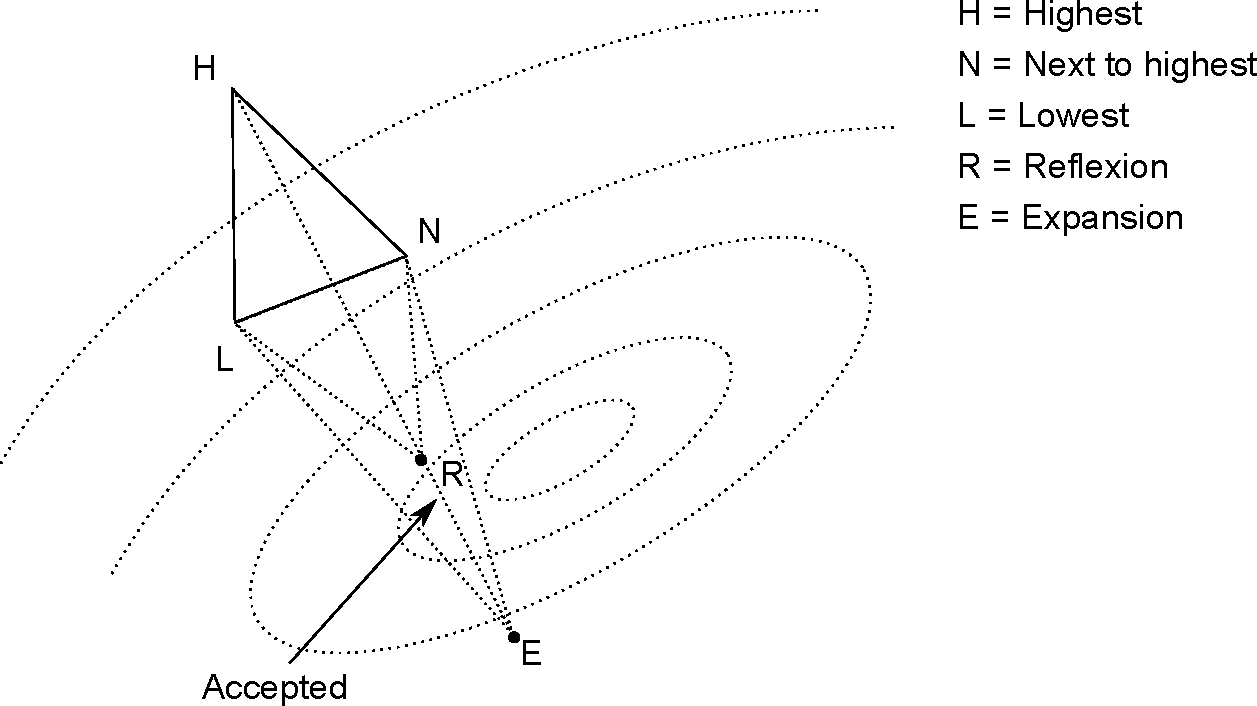
\includegraphics[width=10cm]{nelder-mead-reflection.pdf}
\end{center}
\caption{Nelder-Mead simplex moves -- Reflection}
\label{fig-nm-moves-reflection}
\end{figure}

\begin{figure}
\begin{center}
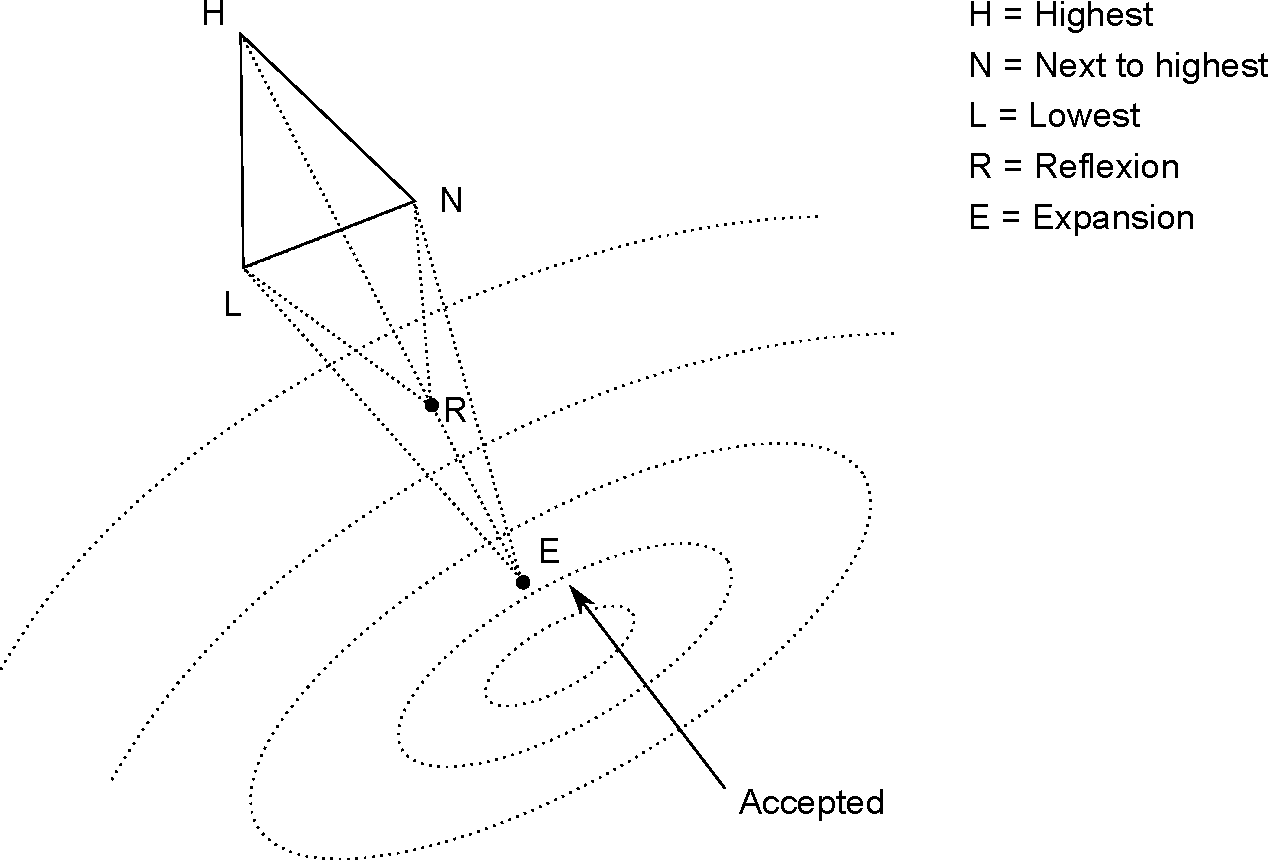
\includegraphics[width=10cm]{nelder-mead-extension.pdf}
\end{center}
\caption{Nelder-Mead simplex moves -- Expansion}
\label{fig-nm-moves-expansion}
\end{figure}

\begin{figure}
\begin{center}
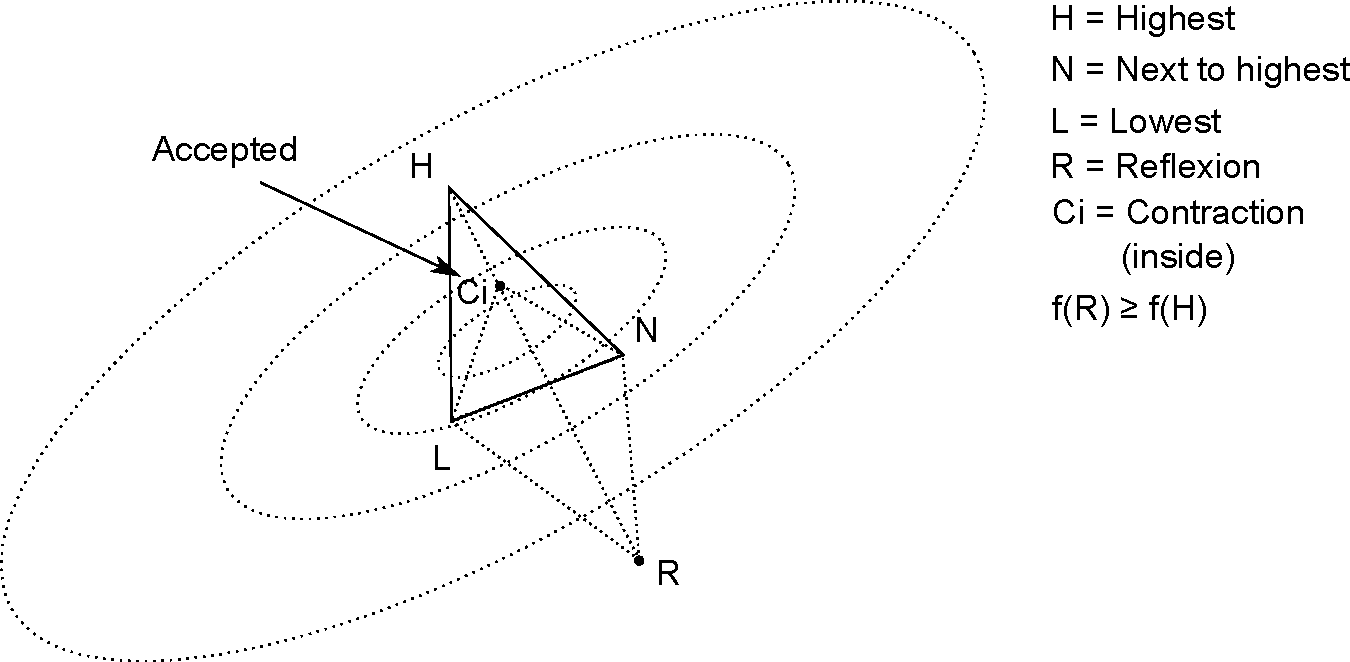
\includegraphics[width=10cm]{nelder-mead-contract-inside.pdf}
\end{center}
\caption{Nelder-Mead simplex moves - Inside contraction}
\label{fig-nm-moves-insidecontraction}
\end{figure}

\begin{figure}
\begin{center}
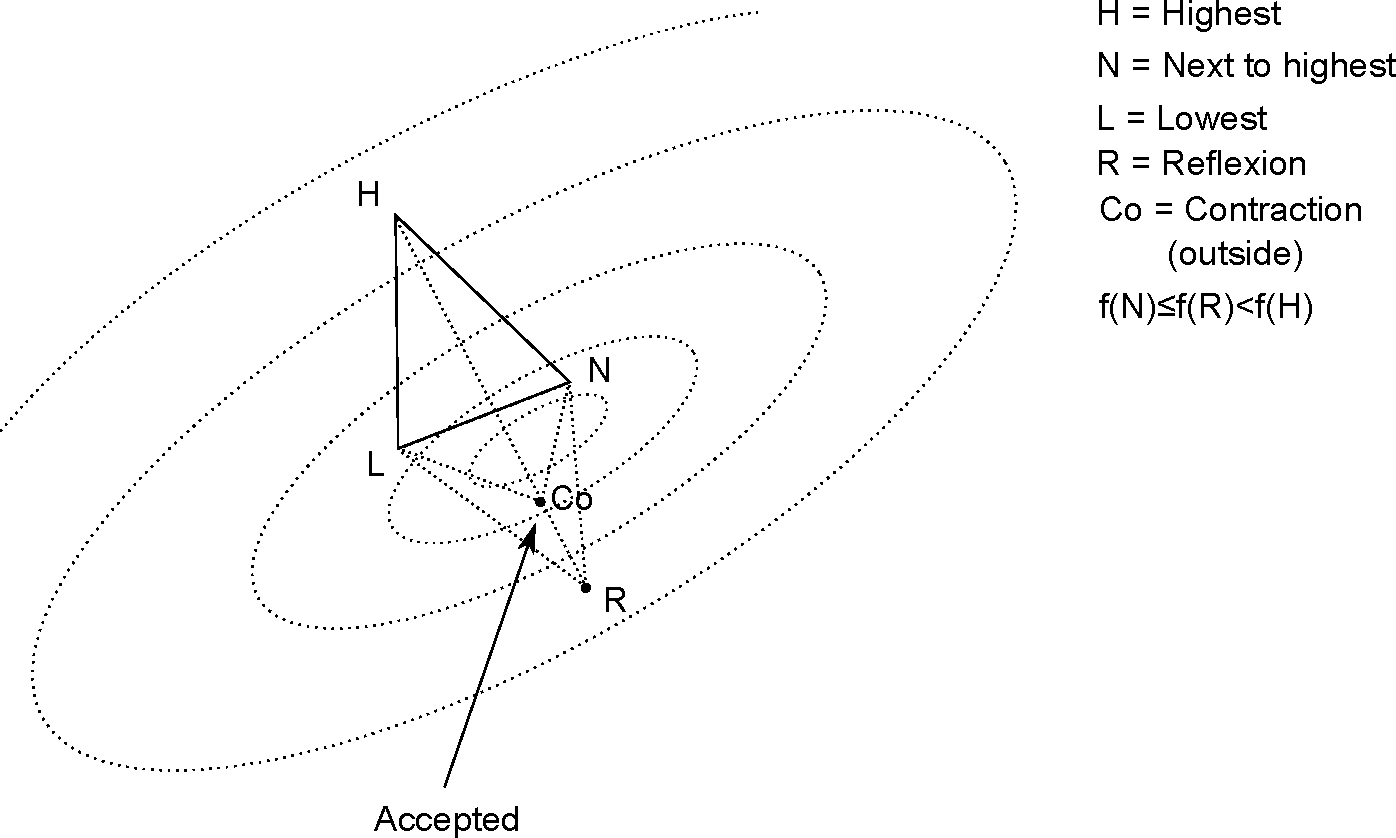
\includegraphics[width=10cm]{nelder-mead-contract-outside.pdf}
\end{center}
\caption{Nelder-Mead simplex moves -- Outside contraction}
\label{fig-nm-moves-outsidecontraction}
\end{figure}

\begin{figure}
\begin{center}
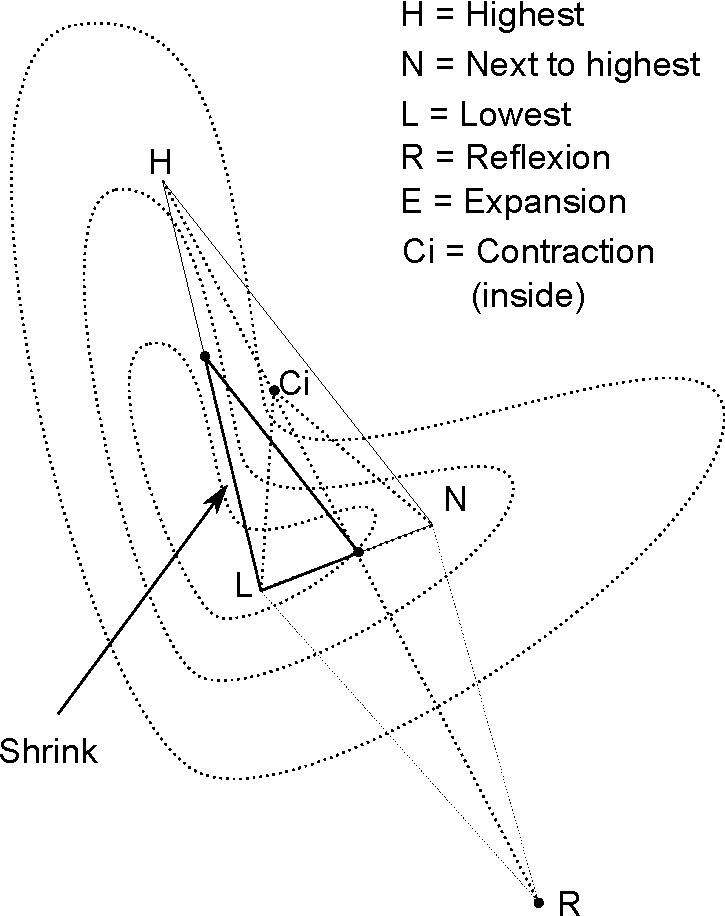
\includegraphics[width=6cm]{nelder-mead-shrink-afterci.pdf}
\end{center}
\caption{Nelder-Mead simplex moves -- Shrink after inside contraction.}
\label{fig-nm-moves-shrinkafterci}
\end{figure}

\begin{figure}
\begin{center}
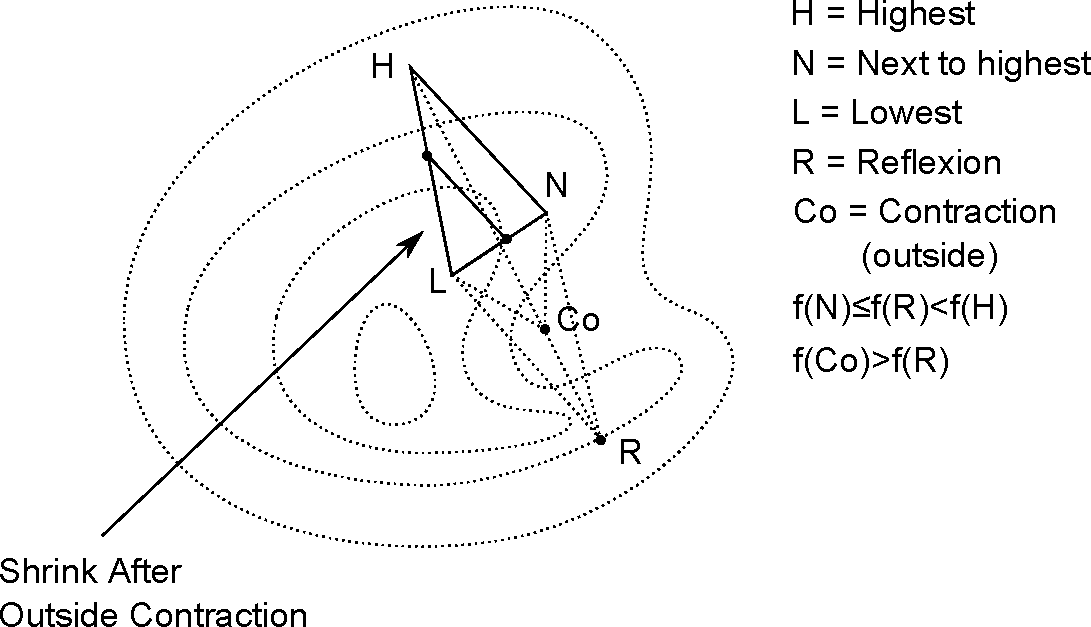
\includegraphics[width=10cm]{nelder-mead-shrink-afterco.pdf}
\end{center}
\caption{Nelder-Mead simplex moves -- Shrink after outside contraction}
\label{fig-nm-moves-shrinkafterco}
\end{figure}


%\subsection{Termination criteria}

%TODO...

\section{Convergence properties on a quadratic}

In this section, we reproduce one result 
presented by Han and Neumann \cite{HanNeumann2006}, which states 
the rate of convergence toward the optimum on a class of quadratic 
functions with a special initial simplex.
Some additional results are also presented in the Phd thesis by Lixing Han \cite{Han2000}.
We study a generalized quadratic and use a particular 
initial simplex. We show that the vertices follow 
a recurrence equation, which is associated with a characteristic 
equation. The study of the roots of these characteristic equations 
give an insight of the behavior of the Nelder-Mead algorithm
when the dimension $n$ increases.

Let us suppose than we want to minimize the function 
\begin{eqnarray}
\label{hanneumman-quadratic}
f(\bx) = x_1^2+\ldots+x_n^2
\end{eqnarray}
with the initial simplex 
\begin{eqnarray}
S_0 = \left[\bold{0},\bv^{(0)}_1,\ldots,\bv^{(0)}_n\right]
\end{eqnarray}
With this choice of the initial simplex, the best vertex remains fixed 
at $\bold{0}=(0,0,\ldots,0)^T\in\RR^n$. As the cost function \ref{hanneumman-quadratic}
is strictly convex, the Nelder-Mead method never performs
the \emph{shrink} step. Therefore, at each iteration, a new simplex 
is formed by replacing the worst vertex $\bv^{(k)}_n$, by a 
new, better vertex. Assume that the Nelder-Mead method 
generates a sequence of simplices $\{S_k\}_{k\geq 0}$ in $\RR^n$,
where 
\begin{eqnarray}
S_k = \left[\bold{0},\bv^{(k)}_1,\ldots,\bv^{(n)}_n\right]
\end{eqnarray}
We wish that the sequence of simplices $S_k\rightarrow \bold{0}\in\RR^n$
as $k\rightarrow \infty$. To measure the progress of convergence,
Han and Neumann use the oriented length $\sigma_+(S_k)$ of the simplex $S_k$,
defined by 
\begin{eqnarray}
\sigma_+(S) = \max_{i=2,m} \|\bv_i - \bv_1\|_2.
\end{eqnarray}
We say that a sequence of simplices $\{S_k\}_{k\geq 0}$ converges to the minimizer $\bold{0}\in\RR^n$
of the function in equation \ref{hanneumman-quadratic} if 
$\lim_{k\rightarrow \infty} \sigma_+(S_k) = 0$.

We measure the rate of convergence defined by 
\begin{eqnarray}
\label{rho-rate-convergence}
\rho(S_0,n) = \textrm{lim sup}_{k\rightarrow \infty} 
\left(\sum_{i=0,k-1} \frac{\sigma(S_{i+1})}{\sigma(S_i)}\right)^{1/k}
\end{eqnarray}
That definition can be viewed as the geometric mean of the ratio of the 
oriented lengths between successive simplices and the minimizer 0.
This definition implies 
\begin{eqnarray}
\label{rho-rate-convergence2}
\rho(S_0,n) = \textrm{lim sup}_{k\rightarrow \infty} 
\left( \frac{\sigma(S_{k+1})}{\sigma(S_0)}\right)^{1/k}
\end{eqnarray}

According to the definition, the algorithm is convergent if $\rho(S_0,n) < 1$.
The larger the $\rho(S_0,n)$, the slower the convergence. In particular, the convergence 
is very slow when $\rho(S_0,n)$ is close to 1. 
The analysis is based on the fact that the Nelder-Mead method generates a sequence of simplices
in $\RR^n$ satisfying 
\begin{eqnarray}
S_k = \left[\bold{0},\bv^{(k+n-1)},\ldots,\bv^{(k+1)},\bv^{(k)}\right],
\end{eqnarray}
where $\bold{0},\bv^{(k+n-1)},\ldots,\bv^{(k+1)},\bv^{(k)}\in\RR^n$ are the vertices
of the $k-th$ simplex, with
\begin{eqnarray}
f(\bold{0}) < f\left(\bv^{(k+n-1)}\right) < f\left(\bv^{(k+1)}\right) < f\left(\bv^{(k)}\right),
\end{eqnarray}
for $k\geq 0$. 

To simplify the analysis, we consider that only one type of step of the Nelder-Mead 
method is applied repeatedly. This allows to establish recurrence equations for the 
successive simplex vertices. As the shrink step is never used, and the expansion steps is 
never used neither (since the best vertex is already at 0), the analysis focuses
on the outside contraction, inside contraction and reflection steps.

The centroid of the $n$ best vertices of $S_k$ is given by 
\begin{eqnarray}
\overline{\bold{v}}^{(k)} 
&=&\frac{1}{n} \left( \bv^{(k+1)} + \ldots + \bv^{(k+n-1)} + \bold{0} \right)\\
&=&\frac{1}{n} \left( \bv^{(k+1)} + \ldots + \bv^{(k+n-1)} \right)\\
&=& \frac{1}{n} \sum_{i=1,n-1} \bv^{(k+i)} \label{eq-nm-centroid}
\end{eqnarray}

\subsection{With default parameters}

In this section, we analyze the roots of the characteristic 
equation with \emph{fixed}, standard inside and outside contraction
coefficients.

\emph{Outside contraction} \\
If the outside contraction step is repeatedly performed
with $\mu_{oc} = \rho\gamma = \frac{1}{2}$, then 
\begin{eqnarray}
\bv^{(k+n)} = \overline{\bold{v}}^{(k)} 
+ \frac{1}{2} \left( \overline{\bold{v}}^{(k)} - \bv^{(k)}\right) .
\end{eqnarray}
By plugging the definition of the centroid \ref{eq-nm-centroid} into the previous equality, we 
find the recurrence formula
\begin{eqnarray}
2n \bv^{(k+n)} - 3 \bv^{(k+1)} - \ldots - 3 \bv^{(k+n-1)} + n\bv^{(k)} = 0.
\end{eqnarray}
The associated characteristic equation is 
\begin{eqnarray}
\label{recurrence-oc}
2n \mu^n - 3 \mu^{n-1} - \ldots - 3 \mu + n = 0.
\end{eqnarray}

\emph{Inside contraction} \\
If the inside contraction step is repeatedly performed
with $\mu_{ic} = -\gamma = -\frac{1}{2}$, then 
\begin{eqnarray}
\bv^{(k+n)} = \overline{\bold{v}}^{(k)} 
- \frac{1}{2} \left( \overline{\bold{v}}^{(k)} - \bv^{(k)}\right).
\end{eqnarray}
By plugging the definition of the centroid \ref{eq-nm-centroid} into the previous equality, we 
find the recurrence formula
\begin{eqnarray}
2n \bv^{(k+n)} - \bv^{(k+1)} - \ldots - \bv^{(k+n-1)} - n\bv^{(k)} = 0.
\end{eqnarray}
The associated characteristic equation is 
\begin{eqnarray}
\label{recurrence-ic}
2n \mu^n - \mu^{n-1} - \ldots - \mu - n = 0.
\end{eqnarray}

\emph{Reflection}  \\
If the reflection step is repeatedly performed
with $\mu_r = \rho = 1$, then 
\begin{eqnarray}
\bv^{(k+n)} = \overline{\bold{v}}^{(k)} 
+ \left( \overline{\bold{v}}^{(k)} - \bv^{(k)}\right).
\end{eqnarray}
By plugging the definition of the centroid \ref{eq-nm-centroid} into the previous equality, we 
find the recurrence formula
\begin{eqnarray}
n \bv^{(k+n)} - 2 \bv^{(k+1)} - \ldots - 2 \bv^{(k+n-1)} + n\bv^{(k)} = 0.
\end{eqnarray}
The associated characteristic equation is 
\begin{eqnarray}
\label{recurrence-reflection}
n \mu^n - 2 \mu^{n-1} - \ldots - 2 \mu + n = 0.
\end{eqnarray}

The recurrence equations \ref{recurrence-oc}, \ref{recurrence-ic} and \ref{recurrence-reflection}
are linear. Their general solutions are of the form 
\begin{eqnarray}
\bv^{(k)} = \mu_1^k \bold{a}_1 + \ldots + \mu_n^k \bold{a}_n,
\end{eqnarray}
where $\{\mu_i\}_{i=1,n}$ are the roots of the characteristic equations and 
$\{\bold{a}_i\}_{i=1,n} \in \CC^n$ are independent vectors such that $\bv^{(k)} \in \RR^n$
for all $k\geq 0$.

The analysis by Han and Neumann \cite{HanNeumann2006} gives a 
deep understanding of the convergence rate for this particular 
situation. For $n=1$, they show that the convergence rate is $\frac{1}{2}$.
For $n=2$, the convergence rate is $\frac{\sqrt{2}}{2}\approx 0.7$ with
a particular choice for the initial simplex. For $n\geq 3$, Han and Neumann \cite{HanNeumann2006}
perform a numerical analysis of the roots.

In the following Scilab script, we compute the roots of these 3 characteristic 
equations. 

\lstset{language=scilabscript}
\begin{lstlisting}
//
// computeroots1 --
//   Compute the roots of the characteristic equations of 
//   usual Nelder-Mead method.
//
function computeroots1 ( n )
  // Polynomial for outside contraction :
  // n - 3x - ... - 3x^(n-1) + 2n x^(n) = 0
  mprintf("Polynomial for outside contraction :\n");
  coeffs = zeros(1,n+1);
  coeffs(1) = n
  coeffs(2:n) = -3
  coeffs(n+1) = 2 * n
  p=poly(coeffs,"x","coeff")
  disp(p)
  mprintf("Roots :\n");
  r = roots(p)
  for i=1:n
    mprintf("Root #%d/%d |%s|=%f\n", i, length(r),string(r(i)),abs(r(i)))
  end
  // Polynomial for inside contraction :
  // - n - x - ... - x^(n-1) + 2n x^(n)= 0
  mprintf("Polynomial for inside contraction :\n");
  coeffs = zeros(1,n+1);
  coeffs(1) = -n
  coeffs(2:n) = -1
  coeffs(n+1) = 2 * n
  p=poly(coeffs,"x","coeff")
  disp(p)
  mprintf("Roots :\n");
  r = roots(p)
  for i=1:n
    mprintf("Root #%d/%d |%s|=%f\n", i, length(r),string(r(i)),abs(r(i)))
  end
  // Polynomial for reflection :
  // n - 2x - ... - 2x^(n-1) + n x^(n) = 0
  mprintf("Polynomial for reflection :\n");
  coeffs = zeros(1,n+1);
  coeffs(1) = n
  coeffs(2:n) = -2
  coeffs(n+1) = n
  p=poly(coeffs,"x","coeff")
  disp(p)
  r = roots(p)
  mprintf("Roots :\n");
  for i=1:n
    mprintf("Root #%d/%d |%s|=%f\n", i, length(r),string(r(i)),abs(r(i)))
  end
endfunction
\end{lstlisting}

If we execute the previous script with $n=10$, the following 
output is produced.

\begin{small}
\begin{verbatim}
-->computeroots1 ( 10 )
Polynomial for outside contraction :
 
                2    3    4    5    6    7    8     9    10  
    10 - 3x - 3x - 3x - 3x - 3x - 3x - 3x - 3x - 3x + 20x    
Roots :
Root #1/10 |0.5822700+%i*0.7362568|=0.938676
Root #2/10 |0.5822700-%i*0.7362568|=0.938676
Root #3/10 |-0.5439060+%i*0.7651230|=0.938747
Root #4/10 |-0.5439060-%i*0.7651230|=0.938747
Root #5/10 |0.9093766+%i*0.0471756|=0.910599
Root #6/10 |0.9093766-%i*0.0471756|=0.910599
Root #7/10 |0.0191306+%i*0.9385387|=0.938734
Root #8/10 |0.0191306-%i*0.9385387|=0.938734
Root #9/10 |-0.8918713+%i*0.2929516|=0.938752
Root #10/10 |-0.8918713-%i*0.2929516|=0.938752
Polynomial for inside contraction :
 
              2   3   4   5   6   7   8    9    10  
  - 10 - x - x - x - x - x - x - x - x - x + 20x    
Roots :
Root #1/10 |0.7461586+%i*0.5514088|=0.927795
Root #2/10 |0.7461586-%i*0.5514088|=0.927795
Root #3/10 |-0.2879931+%i*0.8802612|=0.926175
Root #4/10 |-0.2879931-%i*0.8802612|=0.926175
Root #5/10 |-0.9260704|=0.926070
Root #6/10 |0.9933286|=0.993329
Root #7/10 |0.2829249+%i*0.8821821|=0.926440
Root #8/10 |0.2829249-%i*0.8821821|=0.926440
Root #9/10 |-0.7497195+%i*0.5436596|=0.926091
Root #10/10 |-0.7497195-%i*0.5436596|=0.926091
Polynomial for reflection :
 
                2    3    4    5    6    7    8     9    10  
    10 - 2x - 2x - 2x - 2x - 2x - 2x - 2x - 2x - 2x + 10x    
Roots :
Root #1/10 |0.6172695+%i*0.7867517|=1.000000
Root #2/10 |0.6172695-%i*0.7867517|=1.000000
Root #3/10 |-0.5801834+%i*0.8144859|=1.000000
Root #4/10 |-0.5801834-%i*0.8144859|=1.000000
Root #5/10 |0.9946011+%i*0.1037722|=1.000000
Root #6/10 |0.9946011-%i*0.1037722|=1.000000
Root #7/10 |0.0184670+%i*0.9998295|=1.000000
Root #8/10 |0.0184670-%i*0.9998295|=1.000000
Root #9/10 |-0.9501543+%i*0.3117800|=1.000000
Root #10/10 |-0.9501543-%i*0.3117800|=1.000000
\end{verbatim}
\end{small}

The following Scilab script allows to compute the minimum and 
the maximum of the modulus of the roots. 
The "e" option of the "roots" command has been used to force the 
use of the eigenvalues of the companion matrix as the computational 
method. The default algorithm, based on the Jenkins-Traub Rpoly
method is generating a convergence error and cannot be used 
in this case.

\lstset{language=scilabscript}
\begin{lstlisting}
function [rminoc , rmaxoc , rminic , rmaxic] = computeroots1_abstract ( n )
  // Polynomial for outside contraction :
  // n - 3x - ... - 3x^(n-1) + 2n x^(n) = 0
  coeffs = zeros(1,n+1);
  coeffs(1) = n
  coeffs(2:n) = -3
  coeffs(n+1) = 2 * n
  p=poly(coeffs,"x","coeff")
  r = roots(p , "e")
  rminoc = min(abs(r))
  rmaxoc = max(abs(r))
  // Polynomial for inside contraction :
  // - n - x - ... - x^(n-1) + 2n x^(n)= 0
  coeffs = zeros(1,n+1);
  coeffs(1) = -n
  coeffs(2:n) = -1
  coeffs(n+1) = 2 * n
  p=poly(coeffs,"x","coeff")
  r = roots(p , "e")
  rminic = min(abs(r))
  rmaxic = max(abs(r))
  mprintf("%d & %f & %f & %f & %f\\\\\n", n, rminoc, rmaxoc, rminic, rmaxic)
endfunction

function drawfigure1 ( nbmax )
  rminoctable = zeros(1,nbmax)
  rmaxoctable = zeros(1,nbmax)
  rminictable = zeros(1,nbmax)
  rmaxictable = zeros(1,nbmax)
  for n = 1 : nbmax
    [rminoc , rmaxoc , rminic , rmaxic] = computeroots1_abstract ( n )
    rminoctable ( n ) = rminoc
    rmaxoctable ( n ) = rmaxoc
    rminictable ( n ) = rminic
    rmaxictable ( n ) = rmaxic
  end
  plot2d ( 1:nbmax , [ rminoctable' , rmaxoctable' , rminictable' , rmaxictable' ] )
  f = gcf();
  f.children.title.text = "Nelder-Mead characteristic equation roots";
  f.children.x_label.text = "Number of variables (n)";
  f.children.y_label.text = "Roots of the characteristic equation";
  captions(f.children.children.children,["R-max-IC","R-min-IC","R-max-OC","R-min-OC"]);
  f.children.children(1).legend_location="in_lower_right";
  for i = 1:4
  mypoly = f.children.children(2).children(i);
  mypoly.foreground=i;
  mypoly.line_style=i;
  end
  xs2png(0,"neldermead-roots.png");
endfunction
\end{lstlisting}

For the reflection characteristic equation, the roots all have 
a unity modulus.
The minimum and maximum roots of the inside contraction ("ic" in the table) and 
outside contraction ("oc" in the table) steps are 
presented in table \ref{table-nm-roots-table}. These 
roots are presented graphically in figure \ref{fig-nm-roots}.
We see that the roots start from 0.5 when $n=1$ and 
converge rapidly toward 1 when $n\rightarrow \infty$.

\begin{figure}[htbp]
\begin{center}
\begin{tiny}
\begin{tabular}{|l|l|l|l|l|}
\hline
$n$ & $\min_{i=1,n}\mu_i^{oc}$ & $\max_{i=1,n}\mu_i^{oc}$ & $\min_{i=1,n}\mu_i^{ic}$ & $\max_{i=1,n}\mu_i^{ic}$ \\
\hline
1 & 0.500000 & 0.500000 & 0.500000 & 0.500000\\
2 & 0.707107 & 0.707107 & 0.593070 & 0.843070\\
3 & 0.776392 & 0.829484 & 0.734210 & 0.927534\\
4 & 0.817185 & 0.865296 & 0.802877 & 0.958740\\
5 & 0.844788 & 0.888347 & 0.845192 & 0.973459\\
6 & 0.864910 & 0.904300 & 0.872620 & 0.981522\\
7 & 0.880302 & 0.916187 & 0.892043 & 0.986406\\
8 & 0.892487 & 0.925383 & 0.906346 & 0.989584\\
9 & 0.902388 & 0.932736 & 0.917365 & 0.991766\\
10 & 0.910599 & 0.938752 & 0.926070 & 0.993329\\
11 & 0.917524 & 0.943771 & 0.933138 & 0.994485\\
12 & 0.923446 & 0.948022 & 0.938975 & 0.995366\\
13 & 0.917250 & 0.951672 & 0.943883 & 0.996051\\
14 & 0.912414 & 0.954840 & 0.948062 & 0.996595\\
15 & 0.912203 & 0.962451 & 0.951666 & 0.997034\\
16 & 0.913435 & 0.968356 & 0.954803 & 0.997393\\
17 & 0.915298 & 0.972835 & 0.957559 & 0.997691\\
18 & 0.917450 & 0.976361 & 0.959999 & 0.997940\\
19 & 0.919720 & 0.979207 & 0.962175 & 0.998151\\
20 & 0.922013 & 0.981547 & 0.964127 & 0.998331\\
21 & 0.924279 & 0.983500 & 0.965888 & 0.998487\\
22 & 0.926487 & 0.985150 & 0.967484 & 0.998621\\
23 & 0.928621 & 0.986559 & 0.968938 & 0.998738\\
24 & 0.930674 & 0.987773 & 0.970268 & 0.998841\\
25 & 0.932640 & 0.988826 & 0.971488 & 0.998932\\
26 & 0.934520 & 0.989747 & 0.972613 & 0.999013\\
27 & 0.936316 & 0.990557 & 0.973652 & 0.999085\\
28 & 0.938030 & 0.991274 & 0.974616 & 0.999149\\
29 & 0.939666 & 0.991911 & 0.975511 & 0.999207\\
30 & 0.941226 & 0.992480 & 0.976346 & 0.999259\\
31 & 0.942715 & 0.992991 & 0.977126 & 0.999306\\
32 & 0.944137 & 0.993451 & 0.977856 & 0.999348\\
33 & 0.945495 & 0.993867 & 0.978540 & 0.999387\\
34 & 0.946793 & 0.994244 & 0.979184 & 0.999423\\
35 & 0.948034 & 0.994587 & 0.979791 & 0.999455\\
36 & 0.949222 & 0.994900 & 0.980363 & 0.999485\\
37 & 0.950359 & 0.995187 & 0.980903 & 0.999513\\
38 & 0.951449 & 0.995450 & 0.981415 & 0.999538\\
39 & 0.952494 & 0.995692 & 0.981900 & 0.999561\\
40 & 0.953496 & 0.995915 & 0.982360 & 0.999583\\
45 & 0.957952 & 0.996807 & 0.984350 & 0.999671\\
50 & 0.961645 & 0.997435 & 0.985937 & 0.999733\\
55 & 0.964752 & 0.997894 & 0.987232 & 0.999779\\
60 & 0.967399 & 0.998240 & 0.988308 & 0.999815\\
65 & 0.969679 & 0.998507 & 0.989217 & 0.999842\\
70 & 0.971665 & 0.998718 & 0.989995 & 0.999864\\
75 & 0.973407 & 0.998887 & 0.990669 & 0.999881\\
80 & 0.974949 & 0.999024 & 0.991257 & 0.999896\\
85 & 0.976323 & 0.999138 & 0.991776 & 0.999908\\
90 & 0.977555 & 0.999233 & 0.992236 & 0.999918\\
95 & 0.978665 & 0.999313 & 0.992648 & 0.999926\\
100 & 0.979671 & 0.999381 & 0.993018 & 0.999933\\
\hline
\end{tabular}
\end{tiny}
\end{center}
\caption{Roots of the characteristic equations of the Nelder-Mead method with standard 
coefficients. (Some results are not displayed to make the table fit the page).}
\label{table-nm-roots-table}
\end{figure}

\begin{figure}
\begin{center}
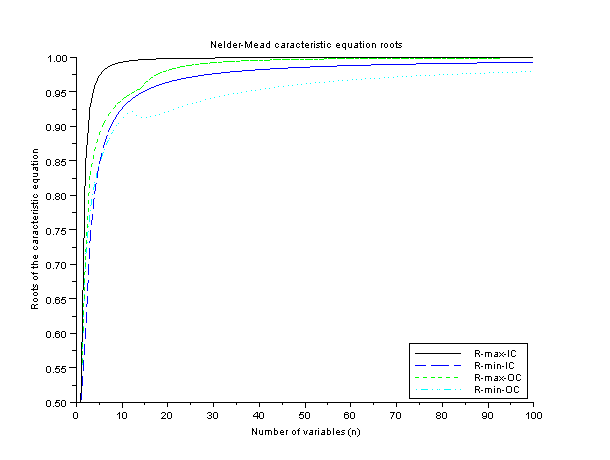
\includegraphics[width=10cm]{neldermead-roots.png}
\end{center}
\caption{Modulus of the roots of the characteristic equations of the Nelder-Mead method with standard 
coefficients -- R-max-IC is the maximum of the modulus of the root of the Inside Contraction steps}
\label{fig-nm-roots}
\end{figure}

\subsection{With variable parameters}

In this section, we analyze the roots of the characteristic 
equation with \emph{variable} inside and outside contraction
coefficients.

\emph{Outside contraction} \\
If the outside contraction step is repeatedly performed
with variable $\mu_{oc} \in }0,\mu_r[$, then 
\begin{eqnarray}
\bv^{(k+n)} &=& \overline{\bold{v}}^{(k)} 
+ \mu_{oc} \left( \overline{\bold{v}}^{(k)} - \bv^{(k)}\right) \\
&=& (1 + \mu_{oc} ) \overline{\bold{v}}^{(k)} - \mu_{oc} \bv^{(k)}
\end{eqnarray}
By plugging the definition of the centroid into the previous equality, we 
find the recurrence formula
\begin{eqnarray}
n \bv^{(k+n)} - (1 + \mu_{oc} ) \bv^{(k+1)} - \ldots - (1 + \mu_{oc} ) \bv^{(k+n-1)} + n\mu_{oc}\bv^{(k)} = 0
\end{eqnarray}

The associated characteristic equation is 
\begin{eqnarray}
\label{recurrence-variable}
n \mu^n - (1 + \mu_{oc} ) \mu^{n-1} - \ldots - (1 + \mu_{oc} ) \mu + n \mu_{oc} = 0.
\end{eqnarray}

\emph{Inside contraction} \\
We suppose that the inside contraction step is repeatedly performed
with $-1 < \mu_{ic} < 0$. The characteristic equation is the same as \ref{recurrence-variable},
but it is here studied in the range $\mu_{ic}\in]-1, 0[$.

To study the convergence of the method, we simply have 
to study the roots of equation \ref{recurrence-variable}, where 
the range $]-1,0[$ corresponds to the inside contraction (with $-1/2$ 
as the standard value) and where the range $]0,\mu_r[$ corresponds to the outside contraction (with $1/2$ 
as the standard value).

In the following Scilab script, we compute the minimum and 
maximum root of the characteristic equation, with $n$ fixed.

\lstset{language=scilabscript}
\begin{lstlisting}
//
// rootsvariable --
//   Compute roots of the characteristic equation 
//   of Nelder-Mead with variable coefficient mu.
// Polynomial for outside/inside contraction :
// n mu - (1+mu)x - ... - (1+mu)x^(n-1) + n x^(n) = 0
//
function [rmin , rmax] = rootsvariable ( n , mu )
  coeffs = zeros(1,n+1);
  coeffs(1) = n * mu
  coeffs(2:n) = -(1+mu)
  coeffs(n+1) = n
  p=poly(coeffs,"x","coeff")
  r = roots(p , "e")
  rmin = min(abs(r))
  rmax = max(abs(r))
  mprintf("%f & %f & %f\\\\\n", mu, rmin, rmax)
endfunction

function drawfigure_variable ( n , nmumax )
  rmintable = zeros(1,nmumax)
  rmaxtable = zeros(1,nmumax)
  mutable = linspace ( -1 , 1 , nmumax ) 
  for index = 1 : nmumax
    mu = mutable ( index )
    [rmin , rmax ] = rootsvariable ( n , mu )
    rmintable ( index ) = rmin
    rmaxtable ( index ) = rmax
  end
  plot2d ( mutable , [ rmintable' , rmaxtable' ] )
  f = gcf();
  pause
  f.children.title.text = "Nelder-Mead characteristic equation roots";
  f.children.x_label.text = "Contraction coefficient";
  f.children.y_label.text = "Roots of the characteristic equation";
  captions(f.children.children.children,["R-max","R-min"]);
  f.children.children(1).legend_location="in_lower_right";
  for i = 1:2
  mypoly = f.children.children(2).children(i);
  mypoly.foreground=i;
  mypoly.line_style=i;
  end
  xs2png(0,"neldermead-roots-variable.png");
endfunction

\end{lstlisting}

The figure \ref{fig-nm-roots-variable} presents the minimum
and maximum modulus of the roots of the characteristic equation
with $n=10$. The result is that when $\mu_{oc}$ is close to 0, the 
minimum root has a modulus close to 0. The maximum root remains close to 
1, whatever the value of the contraction coefficient.
This result would mean that either modifying the contraction
coefficient has no effect (because the maximum modulus of the roots 
is close to 1) or diminishing the contraction coefficient should 
improve the convergence speed (because the minimum modulus of the 
roots gets closer to 0). This is the expected result because
the more the contraction coefficient is close to 0, the more the new 
vertex is close to 0, which is, in our particular situation, the 
global minimizer. No general conclusion can be drawn from this single 
experiment.

\begin{figure}
\begin{center}
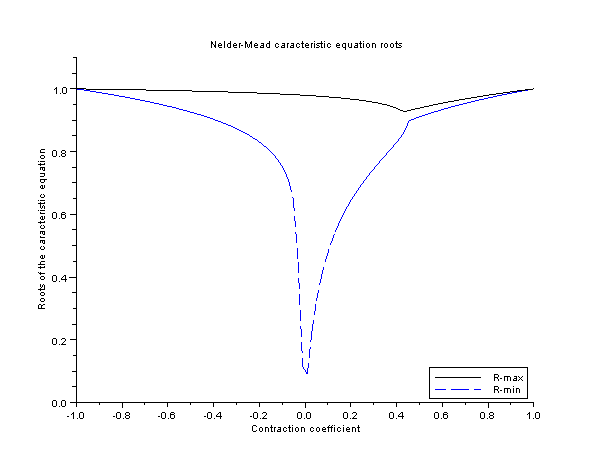
\includegraphics[width=10cm]{neldermead-roots-variable.png}
\end{center}
\caption{Modulus of the roots of the characteristic equations of the Nelder-Mead method with variable 
contraction coefficient and $n=10$ -- R-max is the maximum of the modulus of the root of the 
characteristic equation}
\label{fig-nm-roots-variable}
\end{figure}

\section{Numerical experiments}

In this section, we present some numerical experiments 
with the Nelder-Mead algorithm.
The two first numerical experiments involve simple quadratic functions.
These experiments allows to see the difference between
Spendley's et al. algorithm and the Nelder-Mead algorithm.
We then present several experiments taken from the bibliography.
The O'Neill experiments \cite{O'Neill1971AAF} are performed in order 
to check that our algorithm is a correct implementation.
We then present several numerical experiments where the Nelder-Mead
does not converge properly.
We analyze the Mc Kinnon counter example 
from \cite{589109}. We show the behavior of the 
Nelder-Mead simplex method for a family of examples which cause the 
method to converge to a non stationnary point.
We analyze the counter examples presented by Han in his Phd thesis \cite{Han2000}.
In these experiments, the Nelder-Mead algorithm degenerates by applying repeatedly
the inside contraction step.
We also reproduce numerical experiments extracted from Torczon's Phd Thesis 
\cite{Torczon89multi-directionalsearch}, where Virginia Torczon 
presents the multi-directional direct search algorithm. 

\subsection{Quadratic function}

The function we try to minimize is the following quadratic 
in 2 dimensions 

\begin{eqnarray}
f(x_1,x_2) = x_1^2 + x_2^2 - x_1 x_2
\end{eqnarray}

The stopping criteria is based on the relative size of the simplex 
with respect to the size of the initial simplex 

\begin{eqnarray}
\sigma(S) < tol \times \sigma(S_0)
\end{eqnarray}

The initial simplex is computed from the coordinate axis and the unit length.
The numerical results are presented in table \ref{fig-nm-numexp1-table}.

\begin{figure}[htbp]
\begin{center}
%\begin{tiny}
\begin{tabular}{|l|l|}
\hline
Iterations & 65 \\
Function Evaluations & 127 \\
$x_0$ & $(2.0,2.0)$ \\
Relative tolerance on simplex size & $10^{-8}$ \\
Exact $x^\star$ & $(0.,0.)$\\
Computed $x^\star$ & $(7.3e-10 , -2.5e-9)$\\
Computed $f(x^\star)$ & $8.7e-18$\\
\hline
\end{tabular}
%\end{tiny}
\end{center}
\caption{Numerical experiment with Nelder-Mead method on the quadratic function
$f(x_1,x_2) = x_1^2 + x_2^2 - x_1 x_2$}
\label{fig-nm-numexp1-table}
\end{figure}


The various simplices generated during the iterations are 
presented in figure \ref{fig-nm-numexp1-historysimplex}.
The method use reflections in the early iterations. Then there
is no possible improvement using reflections and shrinking is necessary.

\begin{figure}
\begin{center}
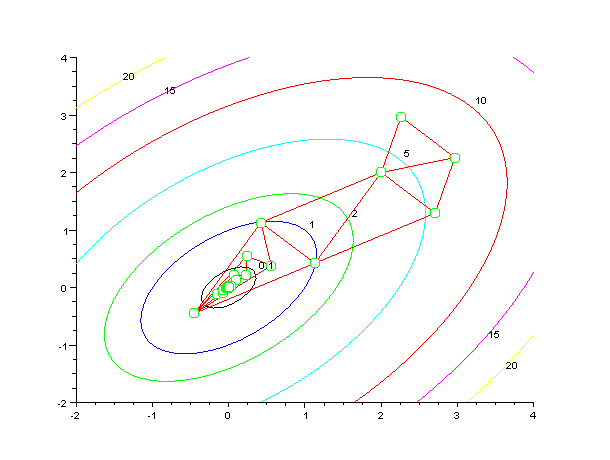
\includegraphics[width=10cm]{quad2bis-nm-simplexcontours.png}
\end{center}
\caption{Nelder-Mead numerical experiment -- history of simplex}
\label{fig-nm-numexp1-historysimplex}
\end{figure}

The figure \ref{fig-nm-numexp1-sigma} presents the history of the oriented
length of the simplex. The length is updated at each iteration, which 
generates a continuous evolution of the length, compared to the 
step-by-step evolution of the simplex with the Spendley et al. algorithm.

\begin{figure}
\begin{center}
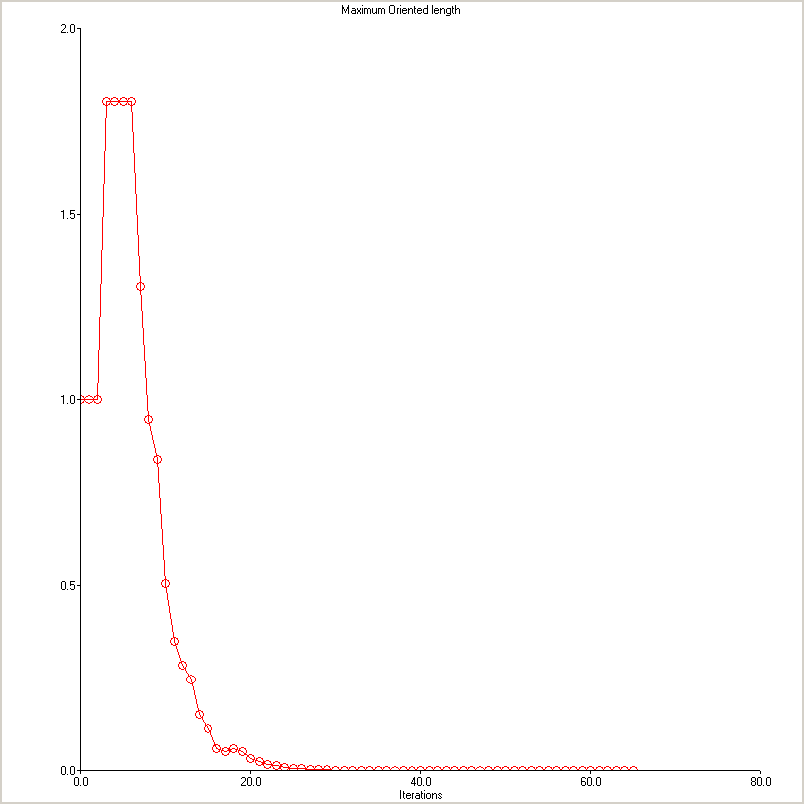
\includegraphics[width=10cm]{quad2bis-nm-history-sigma.png}
\end{center}
\caption{Nelder-Mead numerical experiment -- history of length of simplex}
\label{fig-nm-numexp1-sigma}
\end{figure}

The convergence is quite fast in this case, since less than 60 iterations
allow to get a function value lower than $10^{-15}$, as shown in 
figure \ref{fig-nm-numexp1-logfopt}.

\begin{figure}
\begin{center}
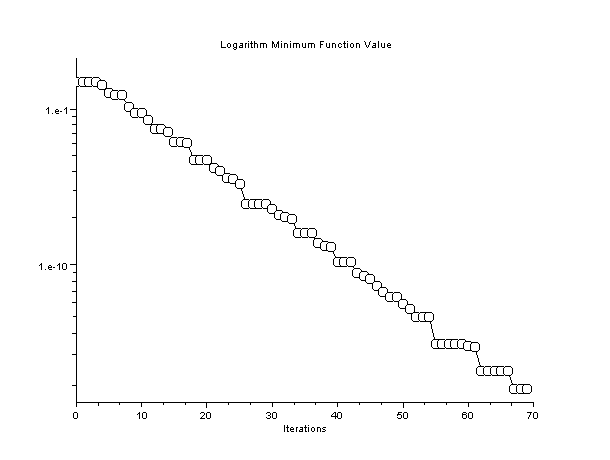
\includegraphics[width=10cm]{quad2bis-nm-history-logfopt.png}
\end{center}
\caption{Nelder-Mead numerical experiment -- history of logarithm of function}
\label{fig-nm-numexp1-logfopt}
\end{figure}

\subsubsection{Badly scaled quadratic function}

The function we try to minimize is the following quadratic 
in 2 dimensions 
\begin{eqnarray}
\label{quadratic-nm-function2}
f(x_1,x_2) = a x_1^2 + x_2^2,
\end{eqnarray}
where $a>0$ is a chosen scaling parameter. 
The more $a$ is large, the more difficult the problem is 
to solve with the simplex algorithm.

We set the maximum number of function evaluations to 400.
The initial simplex is computed from the coordinate axis and the unit length.

The numerical results are presented in table \ref{fig-nm-numexp2-table},
where the experiment is presented for $a=100$. We can check that the 
number of function evaluation (161 function evaluations) is much lower than the number 
for the fixed shape Spendley et al. method (400 function evaluations)
and that the function value at optimum is very accurate ($f(x^\star)\approx 1.e-17$
compared to Spendley's et al. $f(x^\star) \approx 0.08$).

\begin{figure}[h]
\begin{center}
%\begin{tiny}
\begin{tabular}{|l|l|l|}
\hline
& Nelder-Mead & Spendley et al.\\
\hline
Iterations & 83  & 340 \\
Function Evaluations & 161 & 400 \\
$a$ & $100.0$ & - \\
$x_0$ & $(10.0,10.0)$ & - \\
Relative tolerance on simplex size & - \\
Exact $x^\star$ & $(0.,0.)$ & -\\
Computed $x^\star$ & $(2.e-10, -3.e-9)$& $(0.001,0.2)$\\
Computed $f(x^\star)$ & $1.e-17$ & $0.08$\\
\hline
\end{tabular}
%\end{tiny}
\end{center}
\caption{Numerical experiment with Nelder-Mead method on a badly scaled quadratic function.
The variable shape Nelder-Mead algorithm improves the accuracy of the result compared
to the fixed shaped Spendley et al. method.}
\label{fig-nm-numexp2-table}
\end{figure}

In figure \ref{fig-nm-numexp2-scaling}, we analyze the 
behavior of the method with respect to scaling.
We check that the method behave very smoothly, with a very 
small number of additional function evaluations when the 
scaling deteriorates. This shows how much the Nelder-Mead algorithms 
improves over Spendley's et al. method.

\begin{figure}[htbp]
\begin{center}
%\begin{tiny}
\begin{tabular}{|l|l|l|l|}
\hline
$a$ & Function evaluations & Computed $f(x^\star)$ & Computed $x^\star$\\
$1.0$ & 139 & $8.0e-18$ & $(2.e-9 -1.e-9)$\\
$10.0$ & 151 & $7.0e-17$ & $(5.e-10 2.e-9)$\\
$100.0$ & 161 & $1.0e-17$ & $(2.e-10 -3.e-9)$ \\
$1000.0$ & 165 & $1.0e-17$ & $(-1.e-010 9.e-10)$\\
$10000.0$ & 167 & $3.0e-17$ & $(5.0e-11,-1.0e-10)$ \\
\hline
\end{tabular}
%\end{tiny}
\end{center}
\caption{Numerical experiment with Spendley's et al. method on a badly scaled quadratic function}
\label{fig-nm-numexp2-scaling}
\end{figure}

\subsection{Sensitivity to dimension}

In this section, we try to reproduce the result 
presented by Han and Neumann \cite{HanNeumann2006}, which shows that the 
convergence rate of the Nelder-Mead algorithms rapidly 
deteriorates when the number of variables increases.
The function we try to minimize is the following quadratic 
in n-dimensions 
\begin{eqnarray}
\label{quadratic-function3}
f(\bold{x}) = \sum_{i=1,n} x_i^2.
\end{eqnarray}

The initial simplex is computed from the coordinate axis and the unit length.
The initial guess is at 0 so that the first vertex is the origin ; 
this vertex is never updated during the iterations.

The figure \ref{fig-nm-numexp3-dimension} presents the results of this 
experiment for $n=1,19$. 

During the iterations, no shrink steps are performed. The 
algorithm performs reflections, inside and outside contractions.
The figure \ref{fig-nm-numexp3-steps} shows the detailed sequence of 
iterations for $n=10$. We see that there is no general 
pattern for the iterations. One can check, however, that there 
are never no more than $n$ consecutive reflection steps, which is 
as expected. After one or more contractions, the reflection
steps move the worst vertices toward better function values.
But there are only $n+1$ vertices so that the $n$ worst 
vertices are moved in at most $n$ reflection steps.

\begin{figure}[htbp]
\begin{center}
%\begin{tiny}
\begin{verbatim}
I I I I I I I I I I I I I I I I I I I I R R R R R R R R R R R R R I O 
R R R R R R R R R R R R R I R I I R I R O I I I I R I R I I R O I R R 
R R I R I R I R R R R R R R I R R R R I R I I R I R I I I R R I I I R 
R R I R R I R R R R R R I R I R R R R R I R R O R R I O I O R R R R I 
I I O R I R R R R R R I I I R R I I R R R O R I I R R R I R I I O I R 
I R R O I I R R R R I R R O I R R O R I R I R I R R I R I R R R I I I 
I I O R R R R I I I R R R I I I R R R I I I I R R R R I I R R R R I R 
R R I O I R R I I R R R R O I R I I R R R R R R O R R R O I R R I I I 
I O R I I I R I I I I R R I I R R I R R R R R R I R R I I R R O R I I 
O R I R O O R O I I R I I I R I I R R R R R R R R R R R R I R R O I R 
I O I R I I I I R I I R I I R I R O R I O R I R I R R R O R I R R R I 
I R I R R R I R I R R R R I I R R I R R R R I I R R R R I I R I R I I 
O I R I I R R R R R R R R I O I R R I I I R I R I I I I R R R R I R R 
I R I R R R R I I R R R I I I I R I I I I R I R R I R I O R R R I R I 
O I R R I I R R I R R R R O R R R R I O R R R I R I I I I R I R R R R 
R I I R I I R R R R R O R R R I R R R R I R I R R I R I I R R I I R R 
I I I I R R R R R R R R R I R R O R R R R R O I I I I R I I R O I I R 
R R R R I I I R R
\end{verbatim}
%\end{tiny}
\end{center}
\caption{Numerical experiment with Nelder-Mead method on a generalized 
quadratic function - steps of the algorithm : I = inside contraction, O = outside contraction, 
R = reflection, S = shrink}
\label{fig-nm-numexp3-steps}
\end{figure}

The figure \ref{fig-nm-numexp3-nbsteps} presents the number and 
the kind of steps performed during the iterations for $n=1,19$.
It appears that the number of shrink steps and expansion steps is zero, as expected.
More interesting is that the number of reflection is 
larger than the number of inside contraction when $n$ 
is large. The number of outside contraction is always 
the smallest in this case.

\begin{figure}[htbp]
\begin{center}
%\begin{tiny}
\begin{tabular}{|l|l|l|l|l|l|}
\hline
$n$ & \# Reflections & \# Expansion & \# Inside & \# Outside & \#Shrink\\
 & & & Contractions & Contractions & \\
\hline
1 & 0 & 0 & 27 & 0 & 0\\
2 & 0 & 0 & 5 & 49 & 0\\
3 & 54 & 0 & 45 & 36 & 0\\
4 & 93 & 0 & 74 & 34 & 0\\
5 & 123 & 0 & 101 & 33 & 0\\
6 & 170 & 0 & 122 & 41 & 0\\
7 & 202 & 0 & 155 & 35 & 0\\
8 & 240 & 0 & 178 & 41 & 0\\
9 & 267 & 0 & 205 & 40 & 0\\
10 & 332 & 0 & 234 & 38 & 0\\
11 & 381 & 0 & 267 & 36 & 0\\
12 & 476 & 0 & 299 & 32 & 0\\
13 & 473 & 0 & 316 & 42 & 0\\
14 & 545 & 0 & 332 & 55 & 0\\
15 & 577 & 0 & 372 & 41 & 0\\
16 & 635 & 0 & 396 & 46 & 0\\
17 & 683 & 0 & 419 & 52 & 0\\
18 & 756 & 0 & 445 & 55 & 0\\
19 & 767 & 0 & 480 & 48 & 0\\
\hline
\end{tabular}
%\end{tiny}
\end{center}
\caption{Numerical experiment with Nelder-Mead method on a generalized quadratic function -- number 
and kinds of steps performed}
\label{fig-nm-numexp3-nbsteps}
\end{figure}

We check that the number of function evaluations 
increases approximately linearly with the dimension of the problem in
figure \ref{fig-nm-numexp3-fvn}. A rough rule of thumb is that, for $n=1,19$, 
the number of function evaluations is equal to $100n$.

\begin{figure}[htbp]
\begin{center}
%\begin{tiny}
\begin{tabular}{|l|l|l|l|}
\hline
$n$ & Function evaluations & Iterations & $\rho(S_0,n)$\\
\hline
1 & 56 & 28 & 0.5125321059829373\\
2 & 111 & 55 & 0.71491052830553248\\
3 & 220 & 136 & 0.87286283470760984\\
4 & 314 & 202 & 0.91247307800713973\\
5 & 397 & 258 & 0.93107793607270162\\
6 & 503 & 334 & 0.94628781077508028\\
7 & 590 & 393 & 0.95404424343636474\\
8 & 687 & 460 & 0.96063768057900478\\
9 & 767 & 513 & 0.96471820169933631\\
10 & 887 & 605 & 0.97000569588245511\\
11 & 999 & 685 & 0.97343652480535203\\
12 & 1151 & 808 & 0.97745310525741003\\
13 & 1203 & 832 & 0.97803465666405531\\
14 & 1334 & 933 & 0.98042500139065414\\
15 & 1419 & 991 & 0.98154526298964495\\
16 & 1536 & 1078 & 0.98305435726547608\\
17 & 1643 & 1155 & 0.98416149958157839\\
18 & 1775 & 1257 & 0.98544909490809807\\
19 & 1843 & 1296 & 0.98584701106083183\\
\hline
\end{tabular}
%\end{tiny}
\end{center}
\caption{Numerical experiment with Nelder-Mead method on a generalized quadratic function}
\label{fig-nm-numexp3-dimension}
\end{figure}

\begin{figure}
\begin{center}
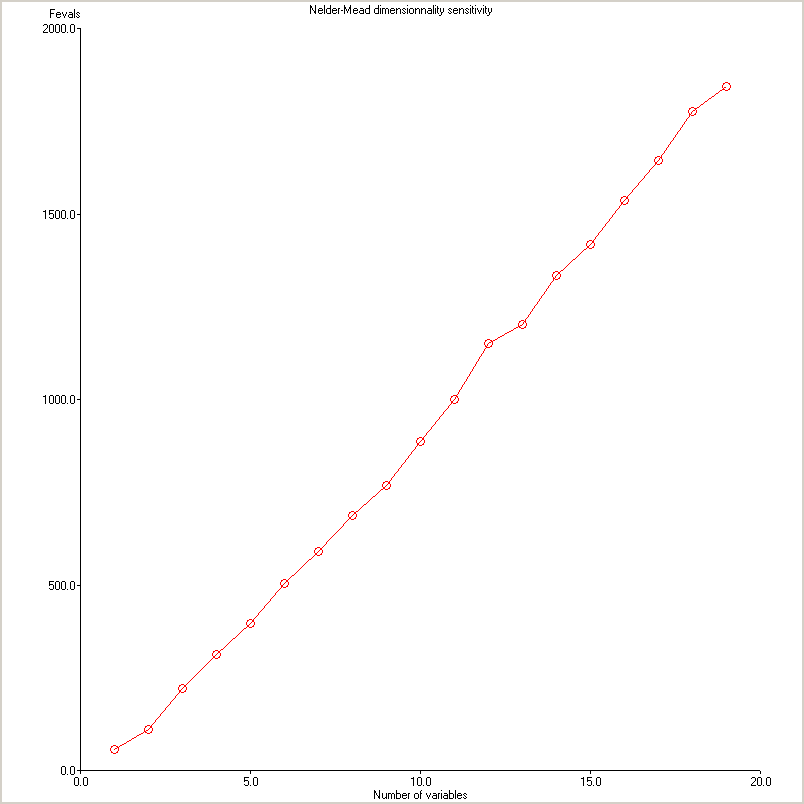
\includegraphics[width=10cm]{neldermead-dimension-nfevals.png}
\end{center}
\caption{Nelder-Mead numerical experiment -- number of function evaluations 
depending on the number of variables}
\label{fig-nm-numexp3-fvn}
\end{figure}

The figure \ref{fig-nm-numexp3-rho} presents the rate of convergence 
depending on the number of variables. The figure shows that 
the rate of convergence rapidly gets close to 1 when the number 
of variables increases. That shows that the rate of convergence 
is slower and slower as the number of variables increases, as 
explained by Han \& Neumann.

\begin{figure}
\begin{center}
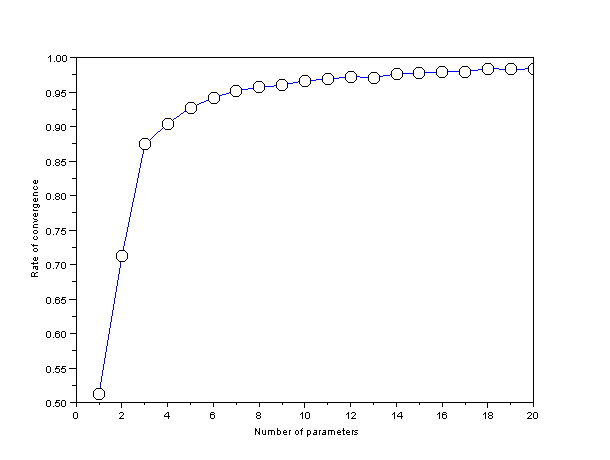
\includegraphics[width=10cm]{neldermead-dimension-rho.png}
\end{center}
\caption{Nelder-Mead numerical experiment -- rate of convergence 
depending on the number of variables}
\label{fig-nm-numexp3-rho}
\end{figure}

\subsection{O'Neill test cases}

In this section, we present the results by O'Neill, who 
implemented a fortran 77 version of the Nelder-Mead algorithm
\cite{O'Neill1971AAF}.

The O'Neill implementation of the Nelder-Mead algorithm has the following 
particularities 
\begin{itemize}
\item the initial simplex is computed from the axes and a (single) length,
\item the stopping rule is based on variance (not standard deviation) of function value,
\item the expansion is greedy, i.e. the expansion point is accepted if it is better than the lower point,
\item an automatic restart is performed if a factorial test shows that the 
computed optimum is greater than a local point computed with a relative 
epsilon equal to 1.e-3.
\end{itemize}

The following tests are presented by O'Neill :

\begin{itemize}
\item Rosenbrock's parabolic valley \cite{citeulike:1903787}
\begin{eqnarray}
\label{nm-oneill-rosenbrock}
f(x_1,x_2) = 100(x_2 - x_1^2)^2 + (1-x_1)^2
\end{eqnarray}
with starting point $(x_1,x_2) = (-1.2,1.0)$
\item Powell's quartic function \cite{Powell08011962}
\begin{eqnarray}
\label{nm-oneill-powell}
f(x_1,x_2,x_3,x_4) = (x_1 + 10x_2)^2 + 5 ( x_3 - x_4)^2 + (x_2 - 2x_3)^4 + 10 (x_1 - x_4)^4
\end{eqnarray}
with starting point $(x_1,x_2,x_3,x_4) = (3,-1,0,1)$
\item Fletcher and Powell's helical valley \cite{R.Fletcher08011963}
\begin{eqnarray}
\label{nm-oneill-fletcherpowell}
f(x_1,x_2,x_3) = 100\left(x_3 + 10\theta(x_1,x_2)\right)^2 
+ \left(\sqrt{x_1^2 + x_2^2} - 1\right)^2  + x_3^2
\end{eqnarray}
where 
\begin{eqnarray}
\label{nm-oneill-fletcherpowelltheta}
2\pi \theta(x_1,x_2) &=& \arctan(x_2,x_1), x_1>0\\
&=& \pi + \arctan(x_2,x_1), x_1<0\\
\end{eqnarray}
with starting point $(x_1,x_2,x_3) = (-1,0,0)$. Note
that since $\arctan(0/0)$ is not defined neither 
the function $f$ on the line $(0,0,x_3)$. This line is excluded 
by assigning a very large value to the function.
\item the sum of powers 
\begin{eqnarray}
\label{nm-oneill-powers}
f(x_1,\ldots,x_{10}) = \sum_{i=1,10} x_i^4
\end{eqnarray}
with starting point $(x_1,\ldots,x_{10}) = (1,\ldots,1)$
\end{itemize}

The parameters are set to 

\begin{itemize}
\item $REQMIN=10^{-16}$, the absolute tolerance on the variance of the function 
values in the simplex,
\item $STEP = 1.0$, the absolute side length of the initial simplex,
\item $ICOUNT$, the maximum number of function evaluations.
\end{itemize}

The table \ref{fig-nm-oneill-table} presents the results which were 
computed by O'Neill compared with our software.
For most experiments, the results are very close in terms of 
number of function evaluations. 
The problem \#4 exhibits a completely different behavior than the 
results presented by O'Neill. For us, the maximum number of function evaluations
is reached (i.e. 1000 function evaluations), whereas for O'Neill, the algorithm 
is restarted and gives the result with 474 function evaluations. 
We did not find any explanation for this behavior. A possible cause of 
difference may be the floating point system which are different and may 
generate different simplices in the algorithms.
Although the CPU times cannot be 
compared (the article is dated 1972 !), let's mention 
that the numerical experiment were performed by O'Neill
on a ICL 4-50 where the two problem 1 and 2 were solved in 3.34 seconds
and the problems 3 and 4 were solved in 22.25 seconds.


\begin{figure}[htbp]
\begin{center}
%\begin{tiny}
\begin{tabular}{|l|l|l|l|l|l|l|}
\hline
Author & Problem & Function & No. of Restarts & Function Value & Iterations & CPU\\
& & Evaluations & & & & Time \\
\hline
O'Neill & 1 & 148 & 0 & 3.19 e-9 & ? & ? \\
Baudin & 1 & 149 & 0 & 1.15 e-7 & 79 & 0.238579 \\
\hline
O'Neill & 2 & 209 & 0 & 7.35 e-8 & ? & ?  \\
Baudin & 2 & 224 & 0 & 1.07 e-8 & 126 & 0.447958 \\
\hline
O'Neill & 3 & 250 & 0 & 5.29 e-9 & ? & ? \\
Baudin & 3 & 255 & 0 & 4.56 e-8 & 137 & 0.627493 \\
\hline
O'Neill & 4 & 474 & 1 & 3.80 e-7 & ? & ? \\
Baudin & 4 & 999 & 0 & 5.91 e-9 & 676 & - \\
\hline
\end{tabular}
%\end{tiny}
\end{center}
\caption{Numerical experiment with Nelder-Mead method on O'Neill test cases - O'Neill results and our results}
\label{fig-nm-oneill-table}
\end{figure}

\subsection{Convergence to a non stationnary point}
\label{section-mcKinnon}

In this section, we analyze the Mc Kinnon counter example 
from \cite{589109}. We show the behavior of the 
Nelder-Mead simplex method for a family of examples which cause the 
method to converge to a non stationnary point.

Consider a simplex in two dimensions with vertices at 0 (i.e. the origin),
$\bv^{(n+1)}$ and $\bv^{(n)}$. Assume that 

\begin{eqnarray}
\label{mckinnon-sortedfv}
f(0) < f(\bv^{(n+1)}) < f(\bv^{(n)}).
\end{eqnarray}

The centroid of the simplex is $\overline{\bv} = \bv^{(n+1)}/2$, the midpoint
of the line joining the best and second vertex. The reflected 
point is then computed as 

\begin{eqnarray}
\label{mckinnon-reflection}
\br^{(n)} = \overline{\bv} + \rho ( \overline{\bv} - \bv^{(n)} ) 
= \bv^{(n+1)} - \bv^{(n)}
\end{eqnarray}

Assume that the reflection point $\br^{(n)}$ is rejected, i.e. that 
$f(\bv^{(n)}) < f(\br^{(n)})$. In this case, the inside contraction 
step is taken and the point $\bv^{(n+2)}$ is computed using the 
reflection factor $-\gamma = -1/2$ so that 

\begin{eqnarray}
\label{mckinnon-insidecontraction}
\bv^{(n+2)} = \overline{\bv} - 
\gamma ( \overline{\bv} - \bv^{(n)} ) 
= \frac{1}{4} \bv^{(n+1)} - \frac{1}{2} \bv^{(n)}
\end{eqnarray}

Assume then that the inside contraction point is accepted, i.e. $f(\bv^{(n+2)}) < f(\bv^{(n+1)})$.
If this sequence of steps repeats, the simplices are subject to the 
following linear recurrence formula

\begin{eqnarray}
\label{mckinnon-reccurence}
4 \bv^{(n+2)} - \bv^{(n+1)} + 2 \bv^{(n)} = 0
\end{eqnarray}

Their general solutions are of the form 

\begin{eqnarray}
\bv^{(n)} = \lambda_1^k a_1 + \lambda_2^k a_2
\end{eqnarray}
where ${\lambda_i}_{i=1,2}$ are the roots of the characteristic equation and 
${a_i}_{i=1,2} \in \RR^n$. 
The characteristic equation is 
\begin{eqnarray}
\label{mckinnon-caracequation}
4 \lambda^2 - \lambda + 2 \lambda = 0
\end{eqnarray}
and has the roots 
\begin{eqnarray}
\label{mckinnon-roots}
\lambda_1 = \frac{1 + \sqrt{33}}{8}\approx 0.84307, 
\qquad \lambda_2 = \frac{1 - \sqrt{33}}{8} \approx -0.59307
\end{eqnarray}

After Mc Kinnon has presented the computation of the roots of the 
characteristic equation, he presents a special initial simplex 
for which the simplices degenerates because of repeated failure by inside 
contraction (RFIC in his article). Consider the initial simplex with
vertices $\bv^{(0)} = (1,1)$ and $\bv^{(1)} = (\lambda_1,\lambda_2)$ and 
$0$. If follows that the particular solution for these initial 
conditions is $\bv^{(n)} = (\lambda_1^n,\lambda_2^n)$.

Consider the function $f(x_1,x_2)$ given by 
\begin{eqnarray}
\label{mckinnon-function}
f(x_1,x_2) &=& \theta \phi |x_1|^\tau + x_2 + x_2^2, \qquad x_1\leq 0,\\
&=&\theta x_1^\tau + x_2 + x_2^2, \qquad x_1\geq 0.
\end{eqnarray}
where $\theta$ and $\phi$ are positive constants. Note that $(0,-1)$
is a descent direction from the origin $(0,0)$ and that f is stricly convex 
provided $\tau>1$. $f$ has continuous first derivatives if $\tau>1$, continuous second 
derivatives if $\tau>2$ and continuous third derivatives if $\tau>3$.

Mc Kinnon computed the conditions on $\theta,\phi$ and $\tau$
so that the function values are ordered as expected, i.e. so that the 
reflection step is rejected and the inside contraction is accepted.
Examples of values which makes these equations hold are as follows :
for $\tau=1$, $\theta=15$ and $\phi = 10$, 
for $\tau=2$, $\theta=6$ and $\phi = 60$ and
for $\tau=3$, $\theta=6$ and $\phi = 400$.

We consider here the more regular case $\tau=3$, $\theta=6$
and $\phi = 400$, i.e. the function is defined by 
\begin{eqnarray}
\label{mckinnon-function3}
f(x_1,x_2) &=& - 2400 x_1^3 + x_2 + x_2^2, \qquad x_1\leq 0, \\
&=& 6 x_1^3 + x_2 + x_2^2, \qquad x_1\geq 0.
\end{eqnarray}

The figure \ref{fig-nm-numexp-mckinnon} shows the contour plot of this function and the first 
steps of the Nelder-Mead method.
The global minimum is located at $(0,-1/2)$.
Notice that the simplex degenerates to the
point $(0,0)$, which is a non stationnary point.

\begin{figure}
\begin{center}
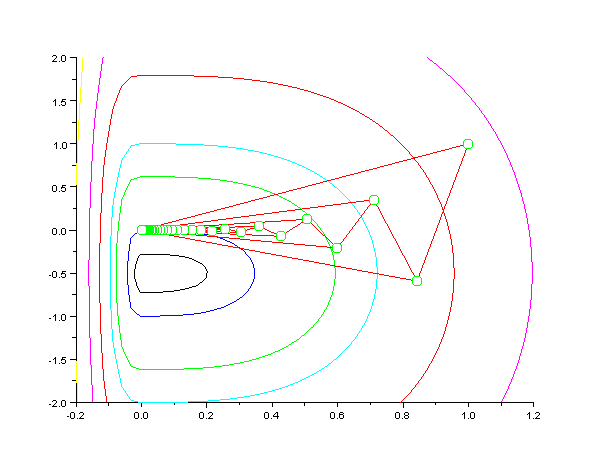
\includegraphics[width=10cm]{mckinnon-history-simplex.png}
\end{center}
\caption{Nelder-Mead numerical experiment -- Mc Kinnon example for convergence toward
a non stationnary point}
\label{fig-nm-numexp-mckinnon}
\end{figure}

The figure \ref{fig-nm-numexp-mckinnon-detail} presents the first steps 
of the algorithm in this numerical experiment. Because of the 
particular shape of the contours of the function, the reflected 
point is always worse that the worst vertex $\bx_{n+1}$. This 
leads to the inside contraction step. The vertices constructed 
by Mc Kinnon are so that the situation loops without end.

\begin{figure}
\begin{center}
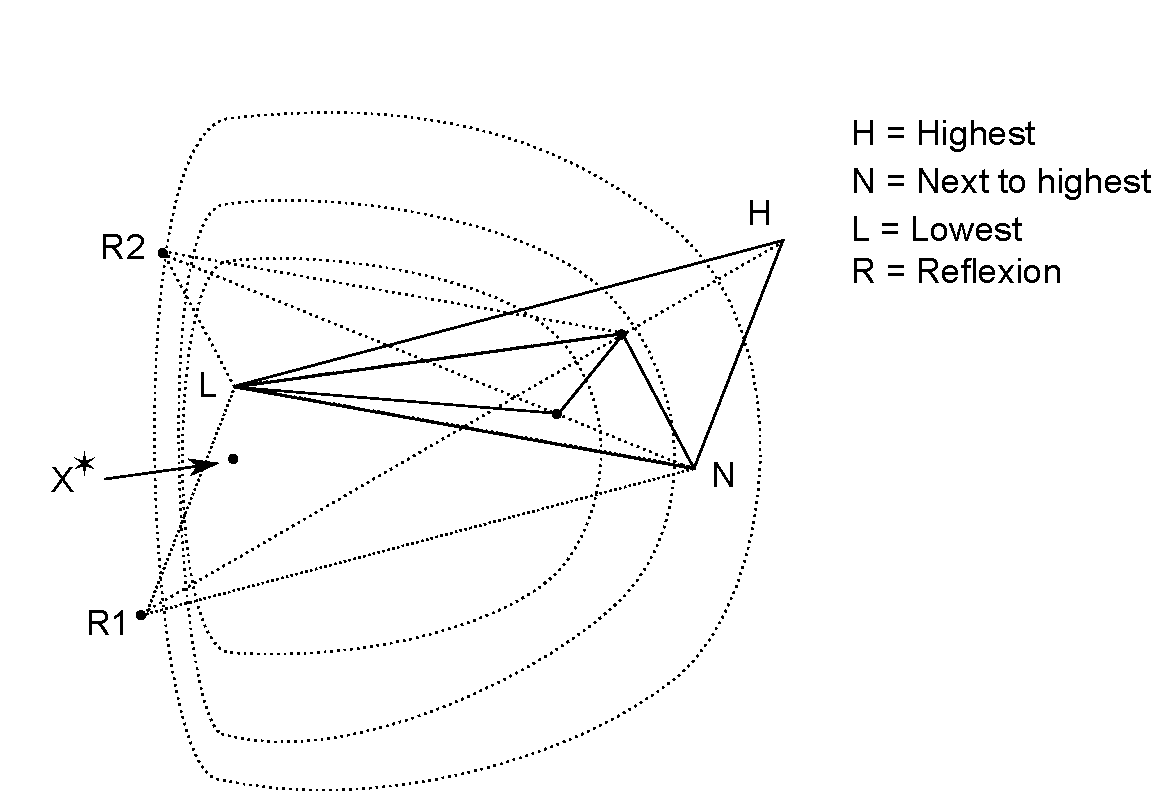
\includegraphics[width=10cm]{mcKinnon-insidecontraction.pdf}
\end{center}
\caption{Nelder-Mead numerical experiment -- Detail of the first steps.
The simplex converges to a non stationnary point, after repeated 
inside contractions.}
\label{fig-nm-numexp-mckinnon-detail}
\end{figure}

\subsection{Han counter examples}

In his Phd thesis \cite{Han2000}, Han presents two counter examples
in which the Nelder-Mead algorithm degenerates by applying repeatedly
the inside contraction step.

\subsubsection{First counter example}

The first counter example is based on the function 
\begin{eqnarray}
\label{han-function1}
f(x_1,x_2) &=& x_1^2 + x_2 ( x_2 + 2 ) ( x_2 - 0.5 ) ( x_2 - 2 )
\end{eqnarray}

This function is nonconvex, bounded below and has bounded level 
sets. The initial simplex is chosen as $S_0 = [(0.,-1),(0,1),(1,0)]$.
Han proves that the Nelder-Mead algorithm generates a sequence of simplices
$S_k = [(0.,-1),(0,1),(\frac{1}{2^k},0)]$.

The figure \ref{fig-nm-numexp-han1} presents the isovalues and the 
simplices during the steps of the Nelder-Mead algorithm.
Note that the limit simplex contains no minimizer of the function.
The failure is caused by repeated inside contractions.

\begin{figure}
\begin{center}
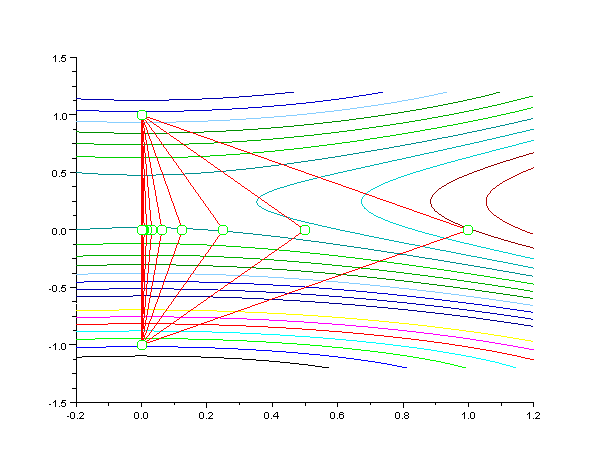
\includegraphics[width=10cm]{han1-history-simplex.png}
\end{center}
\caption{Nelder-Mead numerical experiment -- Han example \#1 for convergence toward
a non stationnary point}
\label{fig-nm-numexp-han1}
\end{figure}

\subsubsection{Second counter example}

The second counter example is based on the function 
\begin{eqnarray}
\label{han-function2}
f(x_1,x_2) &=& x_1^2 + \rho(x_2)
\end{eqnarray}
where $\rho$ is a continuous convex function with bounded level
sets defined by
\begin{eqnarray}
\label{han-function2-rho}
\left\{
\begin{array}{ll}
\rho(x_2) =0, &\qquad \textrm{if} \qquad |x_2|\leq 1, \\
\rho(x_2)\geq 0, &\qquad \textrm{if} \qquad |x_2|> 1.
\end{array}
\right.
\end{eqnarray}
The example given by Han for such a $\rho$ function is 
\begin{eqnarray}
\label{han-function2-rho2}
\rho(x_2) =
\left\{
\begin{array}{ll}
0, &\qquad \textrm{if} \qquad |x_2|\leq 1, \\
x_2 - 1, &\qquad \textrm{if} \qquad x_2> 1, \\
-x_2 - 1, &\qquad \textrm{if} \qquad x_2 < -1.
\end{array}
\right.
\end{eqnarray}

The initial simplex is chosen as $S_0 = [(0.,1/2),(0,-1/2),(1,0)]$.
Han prooves that the Nelder-Mead algorithm generates a sequence of simplices
$S_k = [(0.,1/2),(0,-1/2),(\frac{1}{2^k},0)]$.

The figure \ref{fig-nm-numexp-han2} presents the isovalues and the 
simplices during the steps of the Nelder-Mead algorithm.
The failure is caused by repeated inside contractions.

\begin{figure}
\begin{center}
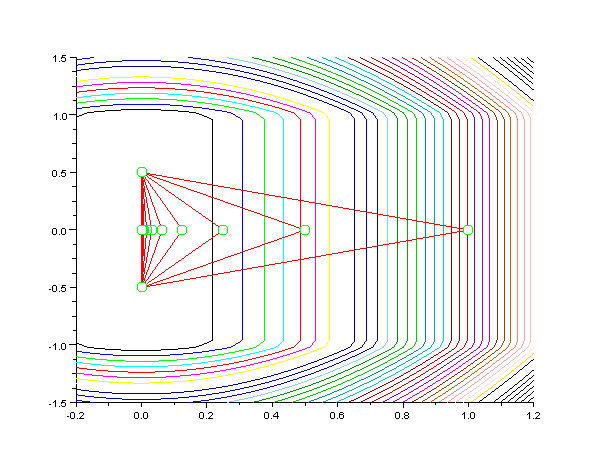
\includegraphics[width=10cm]{han2-history-simplex.png}
\end{center}
\caption{Nelder-Mead numerical experiment -- Han example \#2 for convergence toward
a non stationnary point}
\label{fig-nm-numexp-han2}
\end{figure}

These two examples of non convergence show that the Nelder-Mead method may unreliable.
They also reveal that the Nelder-Mead method can generate simplices which collapse 
into a degenerate simplex, by applying repeated inside contractions.

\subsection{Torczon's numerical experiments}

In her Phd Thesis \cite{Torczon89multi-directionalsearch}, Virginia Torczon 
presents the multi-directional direct search algorithm. In order to analyze the 
performances of her new algorithm, she presents some interesting numerical 
experiments with the Nelder-Mead algorithm. 
These numerical experiments are based on the collection of test problems \cite{355943},
published in the ACM by Mor\'e, Garbow and Hillstrom in 1981. 
These test problems are associated with varying number of variables.
In her Phd, Torczon presents numerical experiments with $n$ from 8 
to 40.
The stopping rule is based on the relative size of the simplex. 
The angle between the descent direction (given by the worst point and the centroid), and the
gradient of the function is computed when the algorithm is stopped.
Torczon shows that, when the tolerance on the relative simplex size is decreased, the 
angle converges toward 90 \degre. This fact is observed even for moderate 
number of dimensions.

In this section, we try to reproduce Torczon numerical experiments.

All experiments are associated with the following sum of squares cost function 
\begin{eqnarray}
\label{torzcon-sumofsquares}
f(\bx) &=& \sum_{i=1,m} f_i(\bx)^2,
\end{eqnarray}
where $m\geq 1$ is the number of functions $f_i$ in the problem.

The stopping criteria is based on the relative size of the 
simplex and is the following 

\begin{eqnarray}
\label{torzcon-stopping}
\frac{1}{\Delta} \max_{i=2,n+1} \|\bv_i - \bv_1\| \leq \epsilon,
\end{eqnarray}
where $\Delta = \max( 1 , \|\bv_1\| )$. Decreasing the value of 
$\epsilon$ allows to get smaller simplex sizes.

\subsubsection{Penalty \#1}
The first test function is the \emph{Penalty \#1} function :

\begin{eqnarray}
\label{torzcon-sumofsquares-case1}
f_i(\bx) &=& \sqrt{1.e-5}(x_i - 1), \qquad i=1,n\\
f_{n+1} & = & -\frac{1}{4} + \sum_{j=1,n} x_j^2.
\end{eqnarray}

The initial guess is given by $\bx_0 = ((\bx_0)_1 , (\bx_0)_2, \ldots , (\bx_0)_n)^T$ and 
$(\bx_0)_j = j$ for $j=1,n$. 

The problem given by 
Mor\'e, Garbow and Hillstrom in \cite{355943} is associated with 
the size $n=4$. The value of the cost function at the initial guess 
$\bx_0 = (1,2,3,4)^T$ is $f(\bx_0) = 885.063$. The value of the function
at the optimum is given in \cite{355943} as $f(\bx^\star) = 2.24997d-5$.
% TODO : what is the optimum ?

Torzcon shows an experiment with the Penalty \#1 test case and $n=8$.
For this particular case, the initial function value is $f(\bx_0) = 4.151406.10^4$.
The figure \ref{fig-nm-torczon-table} presents the results of these
experiments. The number of function evaluations is not the same
so that we can conclude that the algorithm may be different 
variants of the Nelder-Mead algorithms. We were not able to 
explain why the number of function evaluations is so different.

\begin{figure}[htbp]
\begin{center}
%\begin{tiny}
\begin{tabular}{|l|l|l|l|l|}
\hline
Author & Step & $f(\bv_1^\star)$ & Function & Angle (\degre)\\
& Tolerance & & Evaluations & \\
\hline
Torzcon & 1.e-1 & 7.0355e-5 & 1605 & 89.396677792198 \\
Baudin  & 1.e-1 & 8.2272e-5 & 530  & 87.7654 \\
\hline
Torzcon & 1.e-2 & 6.2912e-5 & 1605 & 89.935373548613 \\
Baudin  & 1.e-2 & 7.4854e-5 & 1873 & 89.9253 \\
\hline
Torzcon & 1.e-3 & 6.2912e-5 & 3600 & 89.994626919197 \\
Baudin  & 1.e-3 & 7.4815e-5 & 2135 & 90.0001 \\
\hline
Torzcon & 1.e-4 & 6.2912e-5 & 3670 & 89.999288284747 \\
Baudin  & 1.e-4 & 7.481546e-5 & 2196 & 89.9991 \\
\hline
Torzcon & 1.e-5 & 6.2912e-5 & 3750 & 89.999931862232 \\
Baudin  & 1.e-5 & 7.427212e-5 & 4626 & 89.999990 \\
\hline
\end{tabular}
%\end{tiny}
\end{center}
\caption{Numerical experiment with Nelder-Mead method on Torczon test cases - 
Torczon results and our results}
\label{fig-nm-torczon-table}
\end{figure}

The figure \ref{fig-nm-numexp-torczon1} presents the 
angle between the gradient of the function $-\bg_k$ and the search 
direction $\bx_c - \bx_h$, where $\bx_c$ is the centroid of the best 
vertices and $\bx_h$ is the worst (or high) vertex.

\begin{figure}
\begin{center}
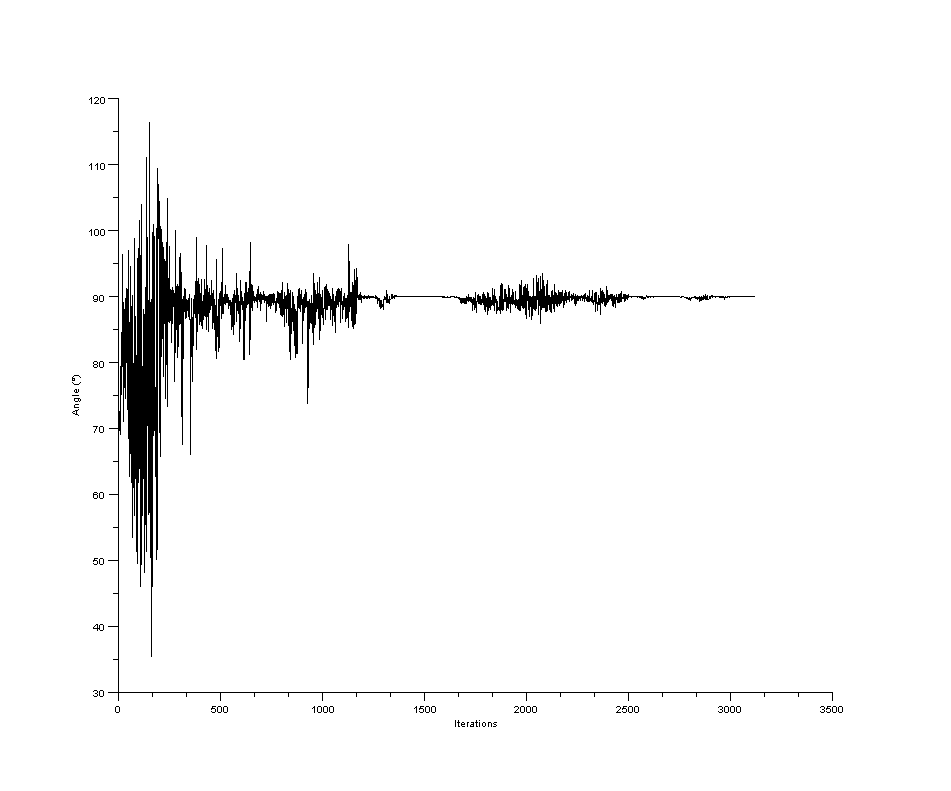
\includegraphics[width=10cm]{torczon_test1_angle.png}
\end{center}
\caption{Nelder-Mead numerical experiment -- Penalty \#1 function --
We see that the angle between the gradient and the search direction
is very close to $90^{\circ}$, especially for large number of iterations.}
\label{fig-nm-numexp-torczon1}
\end{figure}

The numerical experiment shows that the conditioning of the matrix 
of simplex direction has an increasing condition number. This corresponds to the 
fact that the simplex is increasingly distorted.

\section{Conclusion}

The main advantage of the Nelder-Mead algorithm over Spendley et al.
algorithm is that the shape of the simplex is dynamically updated.
That allows to get a reasonably fast convergence rate on badly scaled
quadratics, or more generally when the cost function is made 
of a sharp valley. Nevertheless, the behavior of the algorithm when the 
dimension of the problem increases is disappointing : the more there are 
variables, the more the algorithm is slow. In general, it is expected 
that the number of function evaluations is roughly equal to $100n$.


\chapter{Conclusion}

That tool might be extended in future releases so that it provides the following features :
\begin{itemize}
\item Kelley restart based on simplex gradient [9],
\item C-based implementation (a prototype is provided in appendix B),
\item parallel implementation of the DIRECT algorithm,
\item implementation of the Hook-Jeeves and Multidimensional Search methods [9]
\item parallel implementation of the Nelder-Mead algorithm. See for example [21]. 
?This paper generalizes the widely used Nelder and Mead (Comput J 
7:308?313, 1965) simplex algorithm to parallel processors. Unlike most 
previous parallelization methods, which are based on parallelizing the 
tasks required to compute a specific objective function given a vector 
of parameters, our parallel simplex algorithm uses parallelization at 
the parameter level. Our parallel simplex algorithm assigns to each 
processor a separate vector of parameters corresponding to a point on a 
simplex. The processors then conduct the simplex search steps for an 
improved point, communicate the results, and a new simplex is formed. 
The advantage of this method is that our algorithm is generic and can be 
applied, without re-writing computer code, to any optimization problem 
which the non-parallel Nelder?Mead is applicable. The method is also 
easily scalable to any degree of parallelization up to the number of 
parameters. In a series of Monte Carlo experiments, we show that this 
parallel simplex method yields computational savings in some experiments 
up to three times the number of processors.?
\end{itemize}


\chapter{Acknowledgments}

I would like to thank Vincent Couvert, 
the team manager for Scilab releases, for his support 
during the development of this software. I would like to thank 
Serge Steer, INRIA researcher, for his comments and the discussions 
on this subject. Professor Han, Associate Professor of Mathematics in the 
University of Michigan-Flint University was kind enough to send me a copy
of his Phd and I would like to thank him for that.
My colleagues Allan Cornet and Yann Collette helped me in many 
steps in the long process from the initial idea to the final 
release of the tool and I would like to thank them for their
their time.



\clearpage

%% Appendix
\appendix

\chapter{Nelder-Mead bibliography}

In this section, we present a brief overview of selected 
papers, sorted in chronological order, which deal with 
the Nelder-Mead algorithm

\section{Spendley, Hext, Himsworth, 1962}

"Sequential Application of Simplex Designs in Optimisation and Evolutionary Operation", 
Spendley W., Hext G. R. and Himsworth F. R., 
American Statistical Association and American Society for Quality, 1962

This article \cite{Spendley1962} presents an algorithm for unconstrained optimization in 
which a simplex is used. The simplex has a fixed, regular (i.e. all 
lengths are equal), shape and is made of n+1 vertices (where n is the 
number of parameters to optimize). The algorithm is based on the 
reflection of the simplex with respect to the centroid of better 
vertices. One can add a shrink step so that the simplex size can converge 
to zero. Because the simplex shape cannot change, the convergence rate 
may be very slow if the eigenvalues of the hessian matrix have very 
different magnitude.

\section{Nelder, Mead, 1965}

"A Simplex Method for Function Minimization", 
Nelder J. A.  and Mead R., 
The Computer Journal, 1965

This article \cite{citeulike:3009487} presents the Nelder-Mead unconstrained optimization 
algorithm. It is based on a simplex made of n+1 vertices and is a 
modification of the Spendley's et al algorithm. It includes features 
which enables the simplex to adapt to the local landscape of the cost 
function. The additional steps are expansion, inside contraction and 
outside contraction. The stopping criterion is based on the standard 
deviation of the function value on the simplex.

The convergence of the algorithm is better than Spendley's et al. The 
method is compared against Powell's free-derivative method (1964) with 
comparable behavior. The algorithm is "greedy" in the sense that the 
expansion point is kept if it improves the best function value in the 
current simplex. Most Nelder-Mead variants which have been analyzed 
after are keeping the expansion point only if it improves over the 
reflection point.

\section{Box, 1965}

"A New Method of Constrained Optimization and a Comparison With Other Methods",
M. J. Box,
The Computer Journal 1965 8(1):42-52,
1965, British Computer Society

In this paper \cite{Box1965}, Box presents a modification of the NM algorithm which 
takes into accounts for bound constraints and non-linear constraints.
This variant is called the Complex method. 
The method expects that the initial guess satisfies the nonlinear constraints.
The nonlinear constraints are supposed to define a convex set.
The algorithm ensures that the simplex evolves in the feasible space.

The method to take into account for the bound constraints is based on 
projection of the parameters inside the bounded domain. If some 
nonlinear constraint is not satisfied, the trial point is moved halfway
toward the centroid of the remaining points (which are all satisfying 
the nonlinear constraints).

The simplex may collapse into a subspace if a projection occurs. To 
circumvent this problem, k>=n+1 vertices are used instead of the original 
n+1 vertices. A typical value of k is k=2n. The initial simplex is computed with a random number 
generator, which takes into account for the bounds on the parameters. To 
take into account for the nonlinear constraints, each vertex of the 
initial simplex is moved halfway toward the centroid of the points 
satisfying the constraints (in which the initial guess already is).

\section{Guin, 1968}

"Discussion and correspondence: modification of the complex method of constrained optimization",
J. A. Guin,
The Computer Journal,
1968

In this article \cite{Guin:1968:DCM}, Guin suggest 3 rules to improve the practical convergence 
properties of Box's complex method. These suggestions include the use of the 
next-to-worst point when the worst point does not produce an improvement 
of the function value. The second suggestion is to project the points 
strictly into the bounds, instead of projecting inside the bounds.
The third suggestion is related to the failure of the method
when the centroid is no feasible. In that case, Guin suggest to 
restrict the optimization in the subspace defined by the best 
vertex and the centroid.

\section{O'Neill, 1971}

"Algorithm AS47 - Function minimization using a simplex procedure",
R. O'Neill, 1971, Applied Statistics

In this paper \cite{O'Neill1971AAF}, R. O'Neill presents a fortran 77 implementation of the 
Nelder-Mead algorithm. 
The initial simplex is computed axis-by-axis, given the initial guess
and a vector of step lengths.
A factorial test is used to check if the computed optimum point is a local minimum.

\section{Parkinson and Hutchinson, 1972}

In \cite{parkinson1972}, "An investigation into the efficiency of variants on the simplex method", 
Parkinson and Hutchinson explored 
several ways of improvement. First, they investigate the sensitivity
of the algorithm to the initial simplex. Two parameters were investigated,
i.e. the initial length and the orientation of the simplex. 
An automatic setting for the orientation, though very desirable, is 
not easy to design. Parkinson and Hutchinson tried to automatically 
compute the scale of the initial simplex by two methods, based on 
a "line search" and on a local "steepest descent".
Their second investigation adds a new step to the algorithm, the unlimited
expansion. After a sucessful expansion, the algorithm tries to produce 
an expansion point by taking the largest possible number of 
expansion steps. After an unlimited expansion steps is performed, the 
simplex is translated, so that excessive modification of the scale and shape 
is avoided. Combined and tested against low dimension problems, the 
modified algorithm, named PHS, provides typical gains of 20% gains in 
function evaluations.

\section{Richardson and Kuester, 1973}

"Algorithm 454: the complex method for constrained optimization",
Richardson Joel A. and Kuester J. L.,
Commun. ACM,
1973

In this paper \cite{362324}, Richardson and Kuester shows a fortran 77 implementation
of Box's complex optimization method. The paper clarifies several 
specific points from Box's original paper while remaining very close to it.
Three test problems are presented with the specific algoritmic settings (such as 
the number of vertices for example) and number of iterations.

\section{Shere, 1973}

"Remark on algorithm 454 : The complex method for constrained optimization",
Shere Kenneth D.,
Commun. ACM,
1974

In this article \cite{372783}, Shere presents two counterexamples where the algorithm 454,
implemented by Richardson and Kuester produces an infinite loop.
"This happens whenever the corrected point, the centroid of the remaining 
complex points, and every point on the line segment joining these two points
all have functional values lower than the functional values at each of the
remaining complex points.

\section{Routh, Swartz, Denton, 1977}

"Performance of the Super-Modified Simplex",
M.W. Routh, P.A. Swartz, M.B. Denton,
Analytical Chemistry,
1977

In this article \cite{Routh1977}, 
Routh, Swartz and Denton present a variant
of the Nelder-Mead algorithm, which is called
the Modified Simplex Method (SMS) in their
paper. The algorithm is modified in the following
way. After determination of the worst response (W), 
the responses at the centroid (C) and reflected (R)
vertices are measured and a second-order polynomial
curve is fitted to the responses at W, C and R.
Furthermore, the curve is extrapolated beyond W 
and R by a percentage of the W-R vector resulting
in two types of curve shapes. In the concave down
case, a maximum occurs within the interval.
Assuming a maximization process, evaluation of the
derivative of the curve reveals the location of the
predicted optimum whose response is subsequently
evaluated, the new vertex is located at that position,
and the optimization process is continued.
In the concave up case, a response maximum
does not occur within the interval so the extended
interval boundary producing the highest predicted
response is chosen as the new vertex location,
its response is determined, and the optimization
is continued. If the response at the predicted
extended interval boundary location does not
prove to be greater than the response at R, the 
vertex R may instead be retained as the new 
vertex and the process continued.
The slope at the extended interval boundary
may additionally be evaluated dictating the 
magnitude of the expansion coefficient, i.e.
the greater the slope (indicating rapid approach
to the optimum location), the smaller the required
expansion coefficient and, conversely, the smaller
the slope (indicating remoteness from the 
optimum location), the larger the required expansion
coefficient.

Some additional safeguard procedure must be used
in order to prevent the collapse of the simplex.

\section{Van Der Wiel, 1980}

"Improvement of the Super-Modified Simplex
Optimization Procedure",
P.F.A., Van Der Wiel
Analytica Chimica Acta,
1980

In this article \cite{VanDerWiel1980}, Van Der Wiel
tries to improve the SMS method by Routh et al..
His modifications are based on a Gaussian fit,
weighted reflection point and estimation of response
at the reflection point. Van Der Wiel presents 
a simplified pseudo-code for one algorithm
The method is tested in 5 cases, where the cost
function is depending on the exponential function.

\section{Walters, Parker, Morgan and Deming, 1991}

"Sequential Simplex Optimization for Quality and Productivity in Research, Development, and Manufacturing", 
F. S. Walters, L. R. Parker, Jr., S. L. Morgan, and S. N. Deming, 1991

In this book \cite{WaltersParkerMorganDeming1991}, Walters, Parker, Morgan and Deming
give a broad view on the simplex methods in chemistry. 
The Spendley et al. and Nelder-Mead algorithms are particularily deeply analyzed, 
with many experiments analyzed in great detail.
Template tables are given, so that an engineer can manually perform the optimization
and make the necessary calculations.
Practical advices are given, which allow to make a better use of the algorithms.

In chapter 5, "Comments on Fixed-size and Variable-size Simplexes",
comparing the path of the two algorithms allows to check that a real optimum
has been found.
When the authors analyze the graph produced by the response depending on the number of 
iteration, the general behavior of the fixed-size algorithm is made of four steps.
Gains in response are initially rapid, but the rate of return decreases as the 
simplex probes to find the ridge and then moves along the shallower 
ridge to find the optimum.
The behavior from different starting locations is also analyzed.
Varying the size of the initial simplex is also analyzed for the fixed-size 
simplex algorithm. The many iterations which are produced when a tiny 
initial simplex is used with the fixed-size simplex is emphasized.

The chapter 6, "General Considerations", warns that the user may 
setup an degenerate initial simplex, leading to a false convergence 
of the algorithm. Various other initial simplices are analyzed.
Modifications in the algorithm to take into account for bounds 
contraints are presented.
The behavior of the fixed-size and variable-size simplex algorithms 
is analyzed when the simplex converges.
The "k+1" rule, introduced by Spendley et al. to take into account 
for noise in the cost function is presented.

The chapter 7, "Additional Concerns and Topics" deals with advanced questions 
regarding these algorithms. The variable size simplex algorithm is analyzed
in the situation of a ridge. Partially oscillatory collapse of the 
Nelder-Mead algorithm is presented. The same behavior is 
presented in the case of a saddle point. This clearly shows that 
practionners were aware of the convergence problem of this 
algorithm well before Mc Kinnon presented a simple counter example (in 1998).
The "Massive Contraction" step of Nelder and Mead is presented as a 
solution for this oscillatory behavior. The authors present 
a method, due to Ernst, which allows to keep the volume of the 
simplex, instead of shrinking it. This method is based on a 
translation of the simplex. This modification requires 
$n+1$ function evaluations. A more efficient method, due to King,
is based on reflection with respect to the next-to-worst 
vertex. This modification was first suggested by Spendley et al.
in their fixed-size simplex algorithm.

In the same chapter, the authors present the behavior of the algorithms 
in the case of multiple optima. They also present briefly other 
types of simplex algorithms.

A complete bibliography (from 1962 to 1990) on simplex-based optimization is given in 
the end of the book.

\section{Subrahmanyam, 1989}

"An extension of the simplex method to constrained nonlinear optimization",
M. B. Subrahmanyam, Journal of Optimization Theory and Applications, 1989

In this article \cite{69970}, the simplex algorithm of Nelder and Mead is extended to handle nonlinear 
optimization problems with constraints. To prevent the simplex from 
collapsing into a subspace near the constraints, a delayed reflection is 
introduced for those points moving into the infeasible region. Numerical 
experience indicates that the proposed algorithm yields good results in 
the presence of both inequality and equality constraints, even when the 
constraint region is narrow. 

If a vertex becomes infeasible, we do not increase the value at this 
vertex until the next iteration is completed. Thus, the next iteration
is accomplished using the actual value of the function at the infeasible 
point. At the end of the iteration, in case the previous vertex is not the worst
vertex, it is assigned a high value, so that it then becomes a candidate
for reflection during the next iteration.

The paper presents numerical experiments which are associated with 
thousands of calls to the cost function. This may be related with 
the chosen reflection factor equal to 0.95, which probably cause 
a large number of reflections until the simplex can finally 
satisfy the constraints.

\section{Numerical Recipes in C, 1992}

"Numerical Recipes in C, Second Edition", 
W. H. Press, Saul A. Teukolsky, William T. Vetterling and Brian P. Flannery, 
1992

In this book \cite{NumericalRecipes}, an ANSI C implementation of the Nelder-Mead algorithm is given.
The initial simplex is based on the axis. 
The termination criterion is based on the relative difference of the 
function value of the best and worst vertices in the simplex.

\section{Lagarias, Reeds, Wright, Wright, 1998}

"Convergence Properties of the Nelder--Mead Simplex Method in Low Dimensions", 
Jeffrey C. Lagarias, James A. Reeds, Margaret H. Wright and Paul E. Wright, 
SIAM Journal on Optimization, 1998

This paper \cite{lagarias:112} presents convergence properties of the Nelder-Mead algorithm applied
to stricly convex functions in dimensions 1 and 2. Proofs are given to a minimizer
in dimension 1, and various limited convergence results for dimension 2. 

\section{Mc Kinnon, 1998}

"Convergence of the Nelder--Mead Simplex Method to a Nonstationary Point", 
SIAM J. on Optimization, K. I. M. McKinnon, 1998

In this article \cite{589109}, Mc Kinnon analyzes the behavior of the 
Nelder-Mead simplex method for a family of examples which cause the 
method to converge to a nonstationnary point. All the examples use 
continuous functions of two variables. The family of functions contains
strictly convex functions with up to three continuous derivatives.
In all the examples, the method repeatedly applies the inside 
contraction step with the best vertex remaining fixed. The simplices
tend to a straight line which is orthogonal to the steepest descent 
direction. It is shown that this behavior cannot occur for functions
with more than three continuous derivatives.

\section{Kelley, 1999}

"Detection and Remediation of Stagnation in the Nelder--Mead Algorithm Using a Sufficient Decrease Condition", 
SIAM J. on Optimization, Kelley, C. T., 1999

In this article \cite{589283}, Kelley presents a test for sufficient decrease which, 
if passed for the entire iteration, will guarantee convergence of the 
Nelder-Mead iteration to a stationary point if the objective function is 
smooth. Failure of this condition is an indicator of potential 
stagnation. As a remedy, Kelley propose to restart the algorithm with an 
oriented simplex, smaller than the previously optimum simplex, but with 
a better shape and which approximates the steepest descent step from the 
current best point. The method is experimented against Mc Kinnon test 
function and allow to converge to the optimum, where the original Nelder
-Mead algorithm was converging to a non-stationary point. Although the 
oriented simplex works well in practice, other strategies may be chosen 
with similar results, such as a simplex based on axis, a regular simplex 
(like Spendley's) or a simplex based on the variable magnitude (like 
Pfeffer's suggestion in Matlab's fminsearch). The paper also shows one 
convergence theorem which prove that if the sufficient decrease 
condition is satisfied and if the product of the condition of the simplex 
by the simplex size converge to zero, therefore, with additional 
assumptions on the cost function and the sequence of simplices, any 
accumulation point of the simplices is a critical point of f.

The same ideas are presented in the book \cite{Kelley1999}.

\section{Han, 2000}

In his Phd thesis \cite{Han2000}, Lixing Han analyzes the 
properties of the Nelder-Mead algorithm.
Han present two examples in which the Nelder-Mead 
simplex method does not converge to a single point. 
The first example is a nonconvex function with bounded 
level sets and it exhibits similar nonconvergence properties 
with the Mc Kinnon counterexample $f(\xi_1,\xi_2) = \xi_1^2 - \xi_2(\xi_2-2)$. 
The second example is a convex function with bounded level sets, for 
which the Nelder-Mead simplices converge to a degenerate simplex, but 
not to a single point. These nonconvergent examples support the 
observations by some practitionners that in the Nelder-Mead 
simplices may collapse into a degenerate simplex and therefore support 
the use of a restart strategy. Han also investigates 
the effect of the dimensionality of the Nelder-Mead method.
It is shown that the Nelder-Mead simplex method becomes less
efficient as the dimension increases. Specifically, Han consider the quadratic
function $\xi_1^2 + \ldots + \xi_1^n$ and shows that the Nelder-Mead 
method becomes less efficient as the dimension increases.
The considered example offers insight into understanding the effect
of dimensionnality on the Nelder-Mead method.
Given all the known failures and inefficiencies of the Nelder-Mead 
method, a very interesting question is why it is so popular in practice.
Han present numerical results of the Nelder-Mead method on the standard
collection of Mor\'e-Garbow-Hillstrom with dimensions $n\leq 6$.
Han compare the Nelder-Mead method with a finite difference BFGS 
method and a finite difference steepest descent method. The numerical
results show that the Nelder-Mead method is much more efficient 
than the finite difference steepest descent method for the problems he
tested with dimensions $n\leq 6$. It is also often comparable with the 
finite difference BFGS method, which is believed to be the 
best derivative-free method.
Some of these results are reproduced in \cite{HanNeumann2006} by Han and Neumann, 
"Effect of dimensionality on the Nelder-��Mead simplex method"
and in \cite{hanNeumann2003}, "On the roots of certain polynomials arising 
from the analysis of the Nelder-Mead simplex method".

\section{Nazareth, Tseng, 2001}

"Gilding the Lily: A Variant of the Nelder-Mead Algorithm Based on Golden-Section Search"
Computational Optimization and Applications, 2001, 
Larry Nazareth and Paul Tseng

The article \cite{584536} propose a variant of the Nelder-Mead algorithm derived from 
a reinterpretation of univariate golden-section direct search. In the 
univariate case, convergence of the variant can be analyzed analogously 
to golden-section search. 

The idea is based on a particular choice of the reflection, expansion, 
inside and outside contraction parameters, based on the golden ratio. 
This variant of the Nelder-Mead algorithm is called Nelder-Mead-Golden-
Ratio, or NM-GS. In one dimension, the authors exploit the connection 
with golden-search method and allows to prove a convergence theorem on 
unimodal univariate functions. This is marked contrast to the approach 
taken by Lagarias et al. where considerable effort is expended to show 
convergence of the original NM algorithm on strictly convex univariate 
functions. With the NM-GS variant, one obtain convergence in the 
univariate case (using a relatively simple proof) on the broader class 
of unimodal functions. 

In the multivariate case, the authors modify the variant by replacing 
strict descent with fortified descent and maintaining the interior 
angles of the simplex bounded away from zero. Convergence of the 
modified v ariant can be analyzed by applying results for a fortified-
descent simplicial search method. Some numerical experience with the 
variant is reported.

\section{Perry, Perry, 2001}

"A New Method For Numerical Constrained Optimization"
by Ronald N. Perry, Ronald N. Perry,
March 2001

In this report \cite{Perry01anew}, we propose a new method for constraint 
handling that can be applied to established optimization algorithms and 
which significantly improves their ability to traverse through 
constrained space. To make the presentation concrete, we apply the new 
constraint method to the Nelder and Mead polytope algorithm. The 
resulting technique, called SPIDER, has shown great initial promise for 
solving difficult (e.g., nonlinear, nondifferentiable, noisy) 
constrained problems.

In the new method, constraints are partitioned into multiple
levels. A constrained performance, independent of the objective
function, is defined for each level. A set of rules, based on 
these partitioned performances, specify the ordering and 
movement of vertices as they straddle constraint boundaries;
these rules [...] have been shown to significantly aid motion along
constraints toward an optimum. Note that the new approach uses not 
penalty function and thus does not warp the performance surface,
thereby avoiding the possible ill-conditioning of the objective
function typical in penalty methods.

No numerical experiment is presented.

\section{Andersson, 2001}

"Multiobjective Optimization in Engineering Design - Application to fluid Power Systems"
Johan Andersson, 2001

This PhD thesis \cite{Andersson01multiobjectiveoptimization} gives a brief overview of the Complex method by Box in 
section 5.1.

\section{Peters, Bolte, Marschner, N\"{u}ssen and Laur, 2002}

In \cite{590075}, "Enhanced Optimization Algorithms for the Development of Microsystems", 
the authors combine radial basis function interpolation methods 
with the complex algorithm by Box.
Interpolation with radial basis functions is a linear approach
in which the model function $f$ is generated
via the weighted sum of the basis functions $\Phi_i(r)$.
The parameter $r$ describes the distance of the current
point from the center $x_i$ of the ith basis function. It is
calculated via the euclidean norm.
It is named ComplInt strategy. The name stands for
Complex in combination with interpolation. The Complex
strategy due to Box is very well suited for the
combination with radial basis function interpolation
for it belongs to the polyhedron strategies.
The authors presents a test performed on a pratical application, 
which leaded them to the following comment :
"The best result achieved with the ComplInt strategy
is not only around 10\% better than the best result of
the Complex strategy due to Box, the ComplInt also
converges much faster than the Complex does: while
the Complex strategy needs an average of 7506, the
ComplInt only calls for an average of 2728 quality
function evaluations."


\section{Han, Neumann, 2006}

"Effect of dimensionality on the Nelder-Mead simplex method", 
L. Han and M. Neumann (2006), 


In this article \cite{HanNeumann2006}, the effect of dimensionality on the Nelder-Mead algorithm is 
investigated. It is shown that by using the quadratic function $f(x) = x^T*x$, 
the Nelder-Mead simplex method deteriorates as the dimension 
increases. More precisely, in dimension 1, with the quadratic function
$f(x) = x^2$ and a particular choice of the initial simplex, applies 
inside contraction step repeatedly and the convergence rate (as the 
ratio between the length of the simplex at two consecutive steps) is 1/2. 
In dimension 2, with a particular initial simplex, the NM algorithm 
applies outside contraction step repeatedly and the convergence rate is 
$\sqrt(2)/2$.

For n>=3, a numerical experiment is performed on the quadratic function 
with the fminsearch algorithm from Matlab. It is shown that the original 
NM algorithm has a convergence rate which is converging towards 1 when n 
increases. For n=32, the rate of convergence is 0.9912.

\section{Singer, Nelder, 2008}

\url{http://www.scholarpedia.org/article/Nelder-Mead_algorithm}
Singer and Nelder

This article is a complete review of the Nelder-Mead algorithm.
Restarting the algorithm is adviced when a premature termination occurs.


\chapter{Implementations of the Nelder-Mead algorithm}

In the following sections, we analyze the various implementations of the 
Nelder-Mead algorithm. We analyze the Matlab implementation provided 
by the \emph{fminsearch} command. We analyze the matlab algorithm provided by 
C.T. Kelley and the Scilab port by Y. Collette. We 
present the Numerical Recipes implementations. We analyze the O'Neill 
fortran 77 implementation "AS47". The Burkardt implementation is also covered.
The implementation provided in the NAG collection is detailed.
The Nelder-Mead algorithm from the Gnu Scientific Library is analyzed.

\section{Matlab : fminsearch}

The Matlab command fminsearch implements the Nelder-Mead algorithm \cite{MatlabFminsearch}. 
It provides features such as 
\begin{itemize}
\item maximum number of function evaluations,
\item maximum number of iterations,
\item termination tolerance on the function value,
\item termination tolerance on $x$,
\item output command to display the progress of the algorithm.
\end{itemize}

\section{Kelley and the Nelder-Mead algorithm}

C.T. Kelley has written a book \cite{Kelley1999} on optimization method and devotes a 
complete chapter to direct search algorithms, especially the Nelder-Mead 
algorithm. Kelley provides in \cite{KelleyMethodsOptimizationMatlabCodes} 
the Matlab implementation of the 
Nelder-Mead algorithm. That implementation uses the restart strategy 
that Kelley has published in \cite{589283} and which improves the possible 
stagnation of the algorithm on non local optimization points. No tests 
are provided.

The following is extracted from the README provided with these 
algorithms. 

\begin{verbatim}
These files are current as of December 9, 1998.

-----------------

MATLAB/FORTRAN software for Iterative Methods for Optimization

by C. T. Kelley

These M-files are implementations of the algorithms from the book
"Iterative Methods for Optimization", to be published by SIAM,
by C. T. Kelley. The book, which describes the algorithms, is available
from SIAM (service@siam.org). These files can be modified for non-commercial
purposes provided that the authors: 

C. T. Kelley for all MATLAB codes, 
P. Gilmore and T. D. Choi for iffco.f
J. M. Gablonsky for DIRECT

are acknowledged and clear comment lines are inserted
that the code has been changed. The authors assume no no responsibility
for any errors that may exist in these routines.

Questions, comments, and bug reports should be sent to

Professor C. T. Kelley
Department of Mathematics, Box 8205
North Carolina State University
Raleigh, NC 27695-8205

(919) 515-7163
(919) 515-3798 (FAX)

Tim_Kelley@ncsu.edu

\end{verbatim}


From Scilab's point of view, that ?licence? is a problem since it 
prevents the use of the source for commercial purposes.

\section{Nelder-Mead Scilab Toolbox : Lolimot}

The Lolimot project by Yann Collette provide two Scilab-based Nelder-
Mead implementations \cite{LolimotColletteURL}. The first implementation is a Scilab port of 
the Kelley script. The licence problem is therefore not solved by this 
script. The second implementation \cite{NelderMeadColletteURL} implements the restart strategy 
by Kelley. No tests are provided.

\section{Numerical Recipes}

The Numerical Recipes \cite{NumericalRecipes} provides the C source code of an 
implementation of the Nelder-Mead algorithm. Of course, this is a 
copyrighted material which cannot be included in Scilab.

\section{NASHLIB : A19}

Nashlib is a collection of Fortran subprograms from "Compact Numerical 
Methods for Computers; Linear Algebra and Function Minimisation, " by 
J.C. Nash. The subprograms are written without many of the extra 
features usually associated with commercial mathematical software, such 
as extensive error checking, and are most useful for those applications 
where small program size is particularly important. The license is 
public domain.

Nahslib includes one implementation of the Nelder-Mead algorithm \cite{GAMS-A19A20-Desc}, 
\cite{GAMS-A19A20-Source}. It is written in fortran 77. The coding style is "goto"-based and 
may not be easy to maintain.

\section{O'Neill implementations}

The paper \cite{O'Neill1971AAF} by R. O'Neil in the journal of Applied Statistics 
presents a fortran 77 implementation of the Nelder-Mead algorithm. The 
source code itself is available in \cite{O'NeillAS47}. Many of the following 
implementations are based on this primary source code. We were not able 
to get the paper \cite{O'Neill1971AAF} itself.

On his website, John Burkardt gives a fortran 77 source code of the 
Nelder-Mead algorithm \cite{Burkardtasa047}. The following are the comments in the header 
of the source code.

\begin{verbatim}

c  Discussion:
c
c    This routine seeks the minimum value of a user-specified function.
c
c     Simplex function minimisation procedure due to Nelder+Mead(1965),
c     as implemented by O'Neill(1971, Appl.Statist. 20, 338-45), with
c     subsequent comments by Chambers+Ertel(1974, 23, 250-1), Benyon(1976,
c     25, 97) and Hill(1978, 27, 380-2)
c
c    The function to be minimized must be defined by a function of
c    the form
c
c      function fn ( x, f )
c      double precision fn
c      double precision x(*)
c
c    and the name of this subroutine must be declared EXTERNAL in the
c    calling routine and passed as the argument FN.
c
c    This routine does not include a termination test using the
c    fitting of a quadratic surface.
c
c  Modified:
c
c    27 February 2008
c
c  Author:
c
c    FORTRAN77 version by R ONeill
c    Modifications by John Burkardt

\end{verbatim}

The "Bayesian Survival Analysis" book by Joseph G. Ibrahim, Ming-Hui 
Chen, and Debajyoti Sinha provides in \cite{SurvivalBookOptim} a fortran 77 implementation 
of the Nelder-Mead algorithm. The following is the header of the source 
code.

\begin{verbatim}
c     Simplex function minimisation procedure due to Nelder+Mead(1965),
c     as implemented by O'Neill(1971, Appl.Statist. 20, 338-45), with
c     subsequent comments by Chambers+Ertel(1974, 23, 250-1), Benyon(1976,
c     25, 97) and Hill(1978, 27, 380-2)
\end{verbatim}

The O'Neill implementation uses a restart procedure which is 
based on a local axis by axis search for the optimality of the 
computed optimum.

\section{Burkardt implementations}

John Burkardt gives several implementations of the Nelder-Mead 
algorithm
\begin{itemize}
\item in fortran 77 \cite{Burkardtasa047} 
\item in Matlab by Jeff Borggaard \cite{BurkardtNelderMeadMatlab}.
\end{itemize}

\section{NAG Fortran implementation}

The NAG Fortran library provides the E04CCF/E04CCA routines \cite{NAGE04CCF} which
implements the simplex optimization method.
E04CCA is a version of E04CCF that has additional parameters 
in order to make it safe for use in multithreaded applications.
As mentioned in the documentation, "The method tends to be slow, but it 
is robust and therefore very useful for functions that are subject to inaccuracies.".
The termination criteria is based on the standard deviation of the function
values of the simplex.

The specification of the cost function for E04CCA is:
\begin{verbatim}
SUBROUTINE FUNCT ( N, XC, FC, IUSER, RUSER)
\end{verbatim}
where IUSER and RUSER and integer and double precision array, which allow the 
user to supply information to the cost function.
An output routine, called MONIT is called once every iteration in E04CCF/E04CCA.
It can be used to print out the current values of any selection of its parameters 
but must not be used to change the values of the parameters.

\section{GSL implementation}

The Gnu Scientific Library provides two Nelder-Mead implementations.
The authors are Tuomo Keskitalo, Ivo Alxneit and Brian Gough.
The size of the simplex is the root mean square sum of length of vectors 
from simplex center to corner points.
The termination criteria is based on the size of the simplex.

The C implementation of the minimization algorithm is original.
The communication is direct, in the sense that the specific optimization 
algorithm calls back the cost function.
A specific optimization implementation provides four functions : "alloc", "free", "iterate"
and "set". A generic optimizer is created by connecting it to a specific optimizer.
The user must write the loop over the iterations, making successive calls 
to the generic "iterate" function, which, in turns, calls the specific "iterate" 
associated with the specific optimization algorithm. 

The cost function can be provided as three function pointers 
\begin{itemize}
\item the cost function $f$,
\item the gradient $g$,
\item both the cost function and the gradient.
\end{itemize}
Some additional parameters can be passed to these functions.




%% Bibliography

\addcontentsline{toc}{chapter}{Bibliography}
\bibliographystyle{plain}
\bibliography{neldermead}

\end{document}

